% Copyright (C) 2014-2016 by Thomas Auzinger <thomas@auzinger.name>

\documentclass[draft,final]{vutinfth} % Remove option 'final' to obtain debug information.

% Load packages to allow in- and output of non-ASCII characters.
\usepackage{lmodern}        % Use an extension of the original Computer Modern font to minimize the use of bitmapped letters.
\usepackage[T1]{fontenc}    % Determines font encoding of the output. Font packages have to be included before this line.
\usepackage[utf8]{inputenc} % Determines encoding of the input. All input files have to use UTF8 encoding.

% Extended LaTeX functionality is enables by including packages with \usepackage{...}.
\usepackage{amsmath}    % Extended typesetting of mathematical expression.
\usepackage{amssymb}    % Provides a multitude of mathematical symbols.
\usepackage{mathtools}  % Further extensions of mathematical typesetting.
\usepackage{microtype}  % Small-scale typographic enhancements.
\usepackage[inline]{enumitem} % User control over the layout of lists (itemize, enumerate, description).
\usepackage{multirow}   % Allows table elements to span several rows.
\usepackage{booktabs}   % Improves the typesettings of tables.
\usepackage{subcaption} % Allows the use of subfigures and enables their referencing.
\usepackage[ruled,linesnumbered,algochapter]{algorithm2e} % Enables the writing of pseudo code.
\usepackage[usenames,dvipsnames,table]{xcolor} % Allows the definition and use of colors. This package has to be included before tikz.
\usepackage{nag}       % Issues warnings when best practices in writing LaTeX documents are violated.
\usepackage{todonotes} % Provides tooltip-like todo notes.
\usepackage{hyperref}  % Enables cross linking in the electronic document version. This package has to be included second to last.
\usepackage[acronym,toc]{glossaries} % Enables the generation of glossaries and lists fo acronyms. This package has to be included last.
%\usepackage{algorithm2e}
% Define convenience functions to use the author name and the thesis title in the PDF document properties.

\usepackage{listings}
\usepackage{upquote}
 

\usepackage{color}
\definecolor{bluekeywords}{rgb}{0.13,0.13,1}
\definecolor{greencomments}{rgb}{0,0.5,0}
\definecolor{redstrings}{rgb}{0.9,0,0}

\lstdefinelanguage{FSharp}%
{morekeywords={let, new, match, with, rec, open, module, namespace, type, of, member, % 
and, for, while, true, false, in, do, begin, end, fun, function, return, yield, try, %
mutable, if, then, else, cloud, async, static, use, abstract, interface, inherit, finally },
  otherkeywords={ let!, return!, do!, yield!, use!, var, from, select, where, order, by },
  keywordstyle=\color{bluekeywords},
  sensitive=true,
  basicstyle=\ttfamily,
	breaklines=true,
  xleftmargin=\parindent,
  aboveskip=\bigskipamount,
	tabsize=4,
  morecomment=[l][\color{greencomments}]{///},
  morecomment=[l][\color{greencomments}]{//},
  morecomment=[s][\color{greencomments}]{{(*}{*)}},
  morestring=[b]",
  showstringspaces=false,
  literate={`}{\`}1,
  stringstyle=\color{redstrings},
}







\newcommand{\authorname}{Bernhard Rainer} % The author name without titles.
\newcommand{\thesistitle}{Interactive Shape Detection in Out-of-Core Point-Clouds for Assisted User Interactions} % The title of the thesis. The English version should be used, if it exists.

% Set PDF document properties
\hypersetup{
    pdfpagelayout   = TwoPageRight,           % How the document is shown in PDF viewers (optional).
    linkbordercolor = {Melon},                % The color of the borders of boxes around crosslinks (optional).
    pdfauthor       = {\authorname},          % The author's name in the document properties (optional).
    pdftitle        = {\thesistitle},         % The document's title in the document properties (optional).
    pdfsubject      = {Subject},              % The document's subject in the document properties (optional).
    pdfkeywords     = {a, list, of, keywords} % The document's keywords in the document properties (optional).
}

\setpnumwidth{2.5em}        % Avoid overfull hboxes in the table of contents (see memoir manual).
\setsecnumdepth{subsection} % Enumerate subsections.

\nonzeroparskip             % Create space between paragraphs (optional).
\setlength{\parindent}{0pt} % Remove paragraph identation (optional).

\makeindex      % Use an optional index.
\makeglossaries % Use an optional glossary.
%\glstocfalse   % Remove the glossaries from the table of contents.

% Set persons with 4 arguments:
%  {title before name}{name}{title after name}{gender}
%  where both titles are optional (i.e. can be given as empty brackets {}).
\setauthor{}{\authorname}{BSc.}{male}
\setadvisor{Associate Prof. Dipl.-Ing. Dipl.-Ing. Dr.techn.}{Michael Wimmer}{}{male}

% For bachelor and master theses:
%\setfirstassistant{Pretitle}{Forename Surname}{Posttitle}{male}
%\setsecondassistant{Pretitle}{Forename Surname}{Posttitle}{male}
%\setthirdassistant{Pretitle}{Forename Surname}{Posttitle}{male}

% For dissertations:
\setfirstreviewer{Pretitle}{Forename Surname}{Posttitle}{male}
\setsecondreviewer{Pretitle}{Forename Surname}{Posttitle}{male}

% For dissertations at the PhD School and optionally for dissertations:
\setsecondadvisor{Pretitle}{Forename Surname}{Posttitle}{male} % Comment to remove.

% Required data.
\setaddress{Heigerleinstraße 53 8, 1170 Wien}
\setregnumber{0828592}
\setdate{18}{08}{2017} % Set date with 3 arguments: {day}{month}{year}.
\settitle{\thesistitle}{\thesistitle} % Sets English and German version of the title (both can be English or German).
%\setsubtitle{Optional Subtitle of the Thesis}{Optionaler Untertitel der Arbeit} % Sets English and German version of the subtitle (both can be English or German).

% Select the thesis type: bachelor / master / doctor / phd-school.
% Bachelor:
%\setthesis{bachelor}
%
% Master:
\setthesis{master}
\setmasterdegree{dipl.} % dipl. / rer.nat. / rer.soc.oec. / master
%
% Doctor:
%\setthesis{doctor}
%\setdoctordegree{rer.soc.oec.}% rer.nat. / techn. / rer.soc.oec.
%
% Doctor at the PhD School
%\setthesis{phd-school} % Deactivate non-English title pages (see below)

% For bachelor and master:
\setcurriculum{Visual Computing}{Visual Computing} % Sets the English and German name of the curriculum.

% For dissertations at the PhD School:
\setfirstreviewerdata{Affiliation, Country}
\setsecondreviewerdata{Affiliation, Country}


\begin{document}

\frontmatter % Switches to roman numbering.
% The structure of the thesis has to conform to
%  http://www.informatik.tuwien.ac.at/dekanat

\addtitlepage{naustrian} % German title page (not for dissertations at the PhD School).
\addtitlepage{english} % English title page.
\addstatementpage

%\begin{danksagung*}
%\todo{Ihr Text hier.}
%\end{danksagung*}

\begin{acknowledgements*}

This thesis would not have been possible without the help of a handful of engaged people. 
My first and foremost gratitude goes to the VRVis Zentrum für Virtual Reality und Visualisierung for providing me with the opportunity to do an internship and in consequence conduct this thesis. Within the VRVis, I would like to thank the Semantic Modeling and Acquisition (SMAQ) group for integrating me into their team, both on a professional level and amicably. A special thank you goes out to my Aardvark and F\# Gurus Harald Steinlechner, Georg Haaser, and Attila Szabo, whose help and expertise eased the execution of this thesis enormously. 
I would also like to thank Stefan Maierhofer, leader of the SMAQ group, and my project manager Michael Schwärzler for their ideas, continuous support, and proof-reading this thesis. 
\\
A big thank you goes out to Michael Wimmer from the Technische Universität Wien for his supervision on not only this thesis but all preceding courses and practica. 

Thanks to Lisa Kellner, who accompanied me through this thesis on a daily basis as she sat next to me and continuously provided me with feedback on my work. 

Thanks to Phillip Erler, a fellow diploma student, for all the exchange of knowledge on both our thesis’s. 

Last but not least, I would like to thank my friends and family who encouraged me to pursue an academic career and endured my ongoing talks about point clouds and shape detection for the bigger part of a year.

This work was enabled by the Competence Centre VRVis. VRVis is funded by BMVIT, BMWFW, Styria, SFG and Vienna Business Agency in the scope of COMET - Competence Centers for Excellent Technologies (854174) which is managed by FFG.

\end{acknowledgements*}

%\begin{kurzfassung}
%\todo{Ihr Text hier.}
%\end{kurzfassung}

\begin{abstract}

In recent years

This thesis presents an interactive method of shape detection for out-of-core point clouds. By utilizing the results of the shape detection, improvements are proposed to existing two-dimensional interaction metaphors. Usually, shape detection is performed on the whole point cloud. Thus results are obtained after an extended period of time. Instead, the point cloud is split into chunks of neighboring points that can be processed efficiently in near real-time. The user can select such a region of interest for it to be segmented and is provided with feedback within a fraction of a second, thus making the detected geometry usable almost immediately. This geometry, called primitive shapes, is used to improve existing two-dimensional interaction metaphors. Lasso Selection, as well as Volumetric Brush Selection, benefit from the use of primitive shapes to support the interaction, such that only points are selected that lie roughly follow the curvature of the shape. Thus, the selection of unwanted points in the foreground or background is reduced. Point Picking is improved by the use of a primitive shape as support, as only points are pickable that also belong to the detected primitive shape.\textit{Local Level-of-Detail Increment} is a novel interaction that increases the level-of-detail along a primitive shape, such that additional points that would otherwise be culled are rendered as well. 
\\

As modern point clouds can contain billions of points and the memory capacity of consumer PCs is usually insufficient to store all points at all time, a level-of-detail data structure is used to store the point cloud on the hard disc and data is loaded into memory only on use. This thesis uses a functional octree as data structure to store all points and create a level-of-detail representation of the point cloud. The level-of-detail representation of the point cloud, based on the camera's relative position, is used for interactions and rendering of the point cloud, such that distant regions are presented to the user at lower point resolutions. 

\end{abstract}

% Select the language of the thesis, e.g., english or naustrian.
\selectlanguage{english}

% Add a table of contents (toc).
\tableofcontents % Starred version, i.e., \tableofcontents*, removes the self-entry.

% Switch to arabic numbering and start the enumeration of chapters in the table of content.
\mainmatter


\chapter{Introduction}

\section{Motivation}

In recent years, multiple acquisition devices and methods of point clouds from real objects have emerged, such as laser scanners, LIDAR, Microsoft Kinect, or photogrammetric reconstructions. The fields of applications for point clouds include, but are not limited to, documenting geomorphological erosion, monitoring urban and agricultural developments, mapping archeological sites, and generating assets for the entertainment industry. The acquisition techniques produce highly detailed point clouds that contain several millions of points. This enormous data resolution presents several challenges to both the system and the user. 

\par

% Challenges to the system
The size of point-cloud datasets has increased at such a rapid rate that they are now simply too large to fit into system memory, let alone graphics card memory. Therefore, new solutions for out-of-core representations have emerged. In most of these solutions, the point cloud data is cached in one or more structured files on the hard drive and can therefore not be accessed directly. Based on a culling heuristic, chunks of point-cloud data are loaded into memory as needed. This continuous swapping of data yields the disk speed as a potential bottleneck when it comes to performance. However, it also introduces the benefit of only storing chunks of data in memory that are of immediate interest to the user. 

\par

% Challenges to the user
Point-cloud datasets commonly lack structure and contain a lot of unneeded data. Thus, additional processing is required to enrich the data set with semantic information. To improve data quality, additional postprocessing steps must be performed by the user manually, such as removing imperfect regions, extracting regions of interest. However, achieving this task by using classic two-dimensional interaction metaphors can be tedious and cumbersome as the system cannot predict the desired boundaries of the third dimension of the interaction. Without the use of more semantic information, such as the geometric shape of the region of interest, multiple view changes might be necessary to only select desired regions from the three-dimensional scene. 

\par

% Lack of semantic information
A way of introducing semantic information into unstructured point-cloud data is shape detection. The objective is to find regions in point clouds with similar characteristics, such as local curvature and neighborhoods, to help the user understand local and global structures. Current solutions, as presented by Schnabel et al. \cite{schnabel-2007-efficient, schnabel-2007-ransac}, can already produce a precise segmentation of point clouds. The complexity of these algorithms increases with the size of the point cloud, making the computation for billions of points infeasible in real time. However, when looking at raw numbers, the approach delivers promising results in a fraction of a second for point clouds of smaller size (<12,000 points).

\par

This thesis proposes a user-controlled technique for shape detection in small local regions of point clouds. This approach can to deliver semantic information on the local geometry in interactive time. This information is used to improve ordinary two-dimensional interaction metaphors by limiting the set of points available for interaction to those that belong to the selected shape (i.e. closely follow the curvature of the shape). 


\section{Problem Definition}

Modern point clouds can contain millions of points with it's size often exceeding several gigabytes. Usually, consumer PCs do not have the memory capacity to hold the entire point cloud in system memory or video memory. Efficient out-of-core solutions for point clouds are discussed in numerous publications, Scheibelbauer \cite{scheiblauer-thesis}, Elseberg et al. \cite{elseberg2013one} or the Point Cloud Library \cite{rusu20113d}, to only name a few. However, a custom solution is needed that stores point clouds enriched with semantic information.

\par

In scans of urban environments, many structures can be represented in a more memory-efficient way. Points that follow a wall can often be compressed to few triangles. Pillars often share similarities with cylinders. Detecting such shapes is an immense task that scales with the number of points and fails to be executed in real time. When exploring a point cloud, immediate feedback of local geometry is useful, since it introduces additional information to the user. This task cannot be achieved without substantial postprocessing of the point cloud. 

\par

Common two-dimensional interaction metaphors (e.g. mouse) are useful tools when selecting or picking regions from a two-dimensional context. When porting these techniques to 3D, the third dimension (i.e. depth) must be guessed or controlled separately. A region of interest usually is a set of points that are spatial neighboring and create a structural element in the point cloud. Ideally, the selection of such a region is performed by defining a minimal enclosing volume that contains all points. Achieving this selection by using 2D-interaction metaphors only is challenging, as the techniques do not know the desired depth boundaries of the selection region. Therefore, interactions across multiple views are needed to achieve this selection. Methods that use 3D information, such as the volumetric brush presented by Weyrich et al. \cite{weyrich2004post}, can ease selection tasks. By consulting the depth buffer each frame, the brush follows the curvature of the furthermost geometry. However, by reading pixels from the GPU, the rendering process is stalled. This technique reacts to occlusion such that the brush follows the geometry depicted in the depth buffer, rather then the desired structure. Thus, view changes are still required.


\section{Contributions}

The main contribution of this diploma thesis is the implementation of a semi-automated procedure to detect shapes in multiple levels of detail in point clouds. Instead of performing shape detection on the entire point cloud at once, our approach lets the user control the region in which shapes should be detected. By reducing those regions to a suitable size, a well-known shape detection algorithm can return meaningful results in interactive time, such that the user is presented with immediate feedback on the local geometry of the selected region. 

\par

Contribution dynamic epsilon for shape detection based on the regions density. 

\par

Shapes are detected in multiple levels of detail in the point cloud. A clustering algorithm finds shapes in different different regions and levels of detail, based on a similarity heuristic, and creates a larger connected cluster of shapes. This cluster is used to present geometric information on a larger scale to the user, rather than each shape separately. 

\par

This thesis proposes several improvements to commonly known user interactions. \textit{Point picking} and \textit{region selection} are improved by consulting the local geometry of the point cloud to assist the user. By using a shape as support, the interaction dimensions are reduced to the parameter space of the shapes, allowing the user to exclude unwanted points from interactions easily. 

\par

Additionally, a novel interaction technique is introduced that allows the user to increment the level of detail locally along a shape. This helps the user to explore the structure of the point cloud in more detail. 


\section{Structure of the Work}

Chapter \ref{chap:related_work} covers the related work for this thesis, including point-cloud rendering and out-of-core representations, shape detection, and segmentation and advanced user interactions on point clouds. Chapter \ref{chap:octree} describes the octree used for the out-of-core representation of the point cloud, as well as some metrics that further describe the content of an octree node. Chapter \ref{chap:shapeDetection} describes the algorithms used to detect primitive shapes in a point cloud and proposes a technique to cluster similar shapes into one coherent shape cluster for user interactions. Chapter \ref{chap:systemDesign} discusses the application's features, including the user-controlled shape detection and assisted interactions that utilize the detected shapes as support shape. Chapter \ref{chap:implementation} focuses on implementation details in a functional context. Results of the application are presented in Chapter \ref{chap:results}. Chapter \ref{chap:conclusion} concludes this thesis with a reflection on the application and an outlook on future work. 
 
\chapter {Related Work}
\label{chap:related_work}

This chapter gives an overview over work that is related to this thesis. Section \ref{sec:related_work_point_clouds} presents related work on storing and rendering out-of-core point clouds, Section \ref{sec:related_work_shape detection} shows ways on to detected shapes in point clouds. Related work on interactions is presented in Section \ref{sec:related_work_interactions}. 

\section {Out-of-Core Point-Clouds}
\todo{}
\cite{gobbetti2004layered}
\cite{wimmer2006instant}
\cite{wand2007interactive}
\cite{SCHUETZ-2016-POT}
\chapter{Shape Detection}
\label{chap:shapeDetection}


\section{Overview}

This thesis utilizes shape detection to automatically detect primitive shapes for small parts of the point cloud at a time. It is designed in such a way that the user receives immediate feedback of local geometry for the region under the mouse cursor. The approach utilizes an automated shape detection algorithm that is capable of detecting different types of primitive shapes. This algorithm is designed to find shapes in point clouds that consist of several million points within minutes. However, when looking at the performance for smaller samples, results can be achieved at interactive time rates. Section \ref{sec:schnabel} describes the shape detection algorithm in detail. 
\\

Before using the detected shapes for rendering or interactions, the shapes must be postprocesssed. Since some of the shapes are of infinite size, they need to be refitted to encapsulate the corresponding support points and create a minimal boundary. Section \ref{sec:Refitting} describes this task. 
\\

Section \ref{sec:shapeMatching} proposes a set of heuristics to determine if detected primitive shapes originate from the same geometric structure. Section \ref{sec:shapeClustering} explains the usage of this heuristics in order to create larger, homogeneous cluster of shapes, used for interactions. 


\section{Efficient RANSAC for Point-Cloud Shape Detection}
\label{sec:schnabel}

The section gives a brief overview over the algorithm used to detect primitive shapes. 
Schnabel et al. \cite{schnabel-2007-efficient} propose an automated way to detect simple primitive shapes in unstructured point clouds. The point cloud is decomposed into a set of shapes and a set of unused points. The algorithm supports detection of planes, spheres, cylinders, cones, and tori. 

\textbf{RAN}dom \textbf{SA}mpling \textbf{C}onsens (RANSAC) was first discussed by Fischler and Bolles \cite{fischler1981random} as a paradigm for model fitting for image analysis and automated cartography. However, this approach can be generalized for points with an origin other than images. The shape detection utilizes RANSAC to repeatedly take a minimal set of points to build a primitive shape $\Psi$ and checks if the points in the region roughly follow the curvature of the shape. 

\subsection{Minimal sets}

A minimal set describes the set of points that are needed to construct a candidate shape. 
For each type of shape, the following rule applies: A shape is only considered as candidate shape if all points from the minimal set are within a distance $\epsilon$ to the shape and the normal does not deviate from the shape's normal by more than an angle $\alpha$. 

\begin{itemize}
    \item \textbf{Plane}: A plane is constructed from three points $p_0, p_1, p_2$ whose normals do deviate from the plane's normal less than the angle $\alpha$. 
    
    \item \textbf{Sphere}: A sphere is fully defined by two points $p_0, p_1$ with corresponding normal vectors $n_0, n_1$. The center $c$ of the sphere is defined by the midpoint shortest line segment between the parametric lines $p_0 + tn_0$ and $p_1 + sn_1$. The radius is constructed by averaging the distance of $p_0$ and $p1$ to $c$.

    \item \textbf{Cylinder}:
    In order to create a cylinder, a minimal set of two points  $p_0, p_1$ with corresponding normal vectors $n_0, n_1$ is used. The direction $d$ of the axis is established by $d = n_0 \times n_1$. The origin $c$ of the cylinder is created by projecting the parametric lines $p_0 + tn_0$ and $p_1 + sn_1$ onto the plane $d \cdot x = 0$ and taking their intersection as origin $c$. The radius is the shortest distance between $p_0$ and the axis $c + ud$
    
    \item \textbf{Cone}:
    For simplicity, the minimal set for a cone consists of three points $p_0, p_1, p_2$, rather than two. For each point-normal pair, a plane is created. The intersection of the three planes defines the apex $c$. To describe the direction of the axis a plane is constructed from the points \{$c +  \frac{p_0 - c}{||p_0 - c||}$, $c +  \frac{p_1 - c}{||p_1 - c||}$, $c +  \frac{p_2 - c}{||p_2 - c||}$\}. The normal of this plane is the direction $d$ of the cone axis. The opening angle is given as $\omega = \frac{\sum_{i}^{max} (p_i - c)\cdot d}{3}$
    
    \item \textbf{Torus}:
    A minimal set of four points with normals is used, one more than theoretically necessary, However, this eases the computation.
    Two possible rotational axis are found by intersecting the four point-normal lines $p_i +  \lambda n_i$\cite{marshall2001robust}. For each axis, a full torus is estimated, and the torus is chosen that causes the smaller error in respect to the four points. The minor radius is found by projecting the points onto a plane that rotates around the axis. A circle is constructed using three points, whose radius is the minor radius of the torus. The major radius is given as the distance from the circle center to the axis. 


\end{itemize} 

\subsection{Score function}
\label{sec:scorefun}
To only use points that roughly follow the curvature of a candidate shape, only points within a distance $\epsilon$ are taken into account. Furthermore, each point must fulfill a score function to be considered a support point of the shape $\Psi$. 
The score function for each point consists of the following: 
\begin{itemize}
    \item The distance between the point and the shape must be smaller than $\epsilon$.
    \item The normal of the point must not deviate from the normal of the shape more than a given angle $\alpha$.
    \item Among all points that fulfill the previous two conditions, only the subset of points, which creates the largest connected component embedded in the shape,  is considered.
\end{itemize}

All points that are within a distance $\epsilon$ are taken into account. However, only those whose normals do not deviate from the normal of the shape more than a given angle $\alpha$ are considered support points. Additionally, the number of support points must exceed a threshold value $n$ for this shape to be valid. 


\subsection{Performance}

\begin{table}
    \centering
    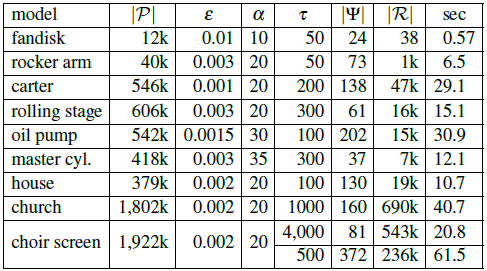
\includegraphics[width=0.7\textwidth]{Shape_Detection/schnabel-performance.png}
    \caption[Original statistics of the shape detection algorithm by Schabel et al.]{The original statistics by Schnabel et al. \cite{schnabel-2007-efficient} on processed models. $\epsilon$ is given as ration of maximum bounding box with. Results have been averaged over 5 runs and rounded.}
    \label{table:schnabel_performance}
\end{table}

Table \ref{table:schnabel_performance} describes the statistical results for different models. $|P|$ is the number of points, $\epsilon$ the distance threshold, $\alpha$ the maximum normals deviation, $\tau$ is the minimum number of support points, $\|Psi|$ the number of shapes found, $|R|$ the number of RANSAC iterations. It can be seen that for small a small number of points and weaker constraints the algorithm returns plausible results within a fraction of a second. We utilize this feature the detect shapes in our application for small regions at a time to give immediate feedback to the user. 


\section{Refitting}
\label{sec:Refitting}

Planes, cylinder, and cones are infinite shapes. Therefore, to use those shapes for rendering and interactions, it is necessary to create finite representations for each shape. Each shape comes with the corresponding set of support points that are used to refit the shape. Spheres and Tori are finite by definition. Therefore they do not require refitting. 


\subsection{Refitting planes}

Planes, however, are represented by a point and a vector. All support points are projected onto the plane, thus reducing the fitting problem to two dimensions. The procedure starts by computing the convex hull of the projected points with the help of Andrew's monotone chain 2d convex hull algorithm\cite{andrew1979another}. 
More complex polygons can be computed. However, for this purpose, a quad is sufficient. The quad is obtained by using the minimum-bounding-rectangle algorithm by Freeman\cite{freeman1975determining}. 


\subsection{Refitting cylinder}

A cylinder is defined by a center $p$, direction vector $v$ and a radius $r$. The height of the cylinder is chosen as the maximum distance between two support points on the axis of the cylinder. This is achieved by projecting all points onto the axis $a = p + vt$ of the cylinder, and select the points $p_{min}$, where $t$ is minimum and $p_{max}$, where $t$ is maximum. The distance $d$ between $p_{min}$ and $p_{max}$ is the height of the enclosing cylinder. The cylinder is refitted such that the new center is set to $p' = p_{min}$ and the $d$ is encoded in the length of the new direction vector:$v' = \frac{v}{|v|}d$. The radius stays the same. 


\subsection{Refitting cones}

A cone is defined by its apex $c$, axis direction $v$, and opening angle $\theta$. Similar to the cylinder, all support points are projected onto the axis and the points $p_{min}, p_{max}$, with minimum and maximum $t$, are selected. Since the apex of a cone is fixed, the range cannot be encoded using $c$ and $v$. The range is stored separately. Range checks are performed when rendering or interacting with cones. 


\section{Shape Detection Parameter Selection}
\label{sec:shapeDetectionParameterSelection}

This section briefly discusses the issue of selecting optimal parameters for the shape detection. The $\epsilon$ parameter creates an $\epsilon$-band that follows the curvature of the shape. All points within this $\epsilon$ band are considered to be candidates. The authors propose to use the point cloud's bounding boxes largest dimension times $0.1$ as $\epsilon$. However, using such a static parameter yields problems with extremely sparse regions and regions that are populated very densely. In this thesis, shape detection is performed dynamically on local regions of the point cloud at a time. The local density of an octree node is chosen as $\epsilon$. The density is calculated per octree node by averaging the distance of each point to its nearest neighbor. Thus, nodes that are populated more densely create finer geometry. 

The $\alpha$ parameter is used to determine the deviation between two directions. As the normals are the same at different level-of-detail, this parameter is static. We use an $\alpha$ value of $0.95$. 

The minimum number of support points per shape is set to $250$.
\chapter{Interactions}

Creating new interactions is a key topic for this thesis. This chapter describes the pros and cons of current state-of-the-art two-dimensional interactions and proposes improvements using the detected primitive shapes as interaction support shapes. 

Many proven interaction techniques have emerged over time, such as \textit{Point Picking} or \textit{Region Selection}. 

%% TODO: define pick ray
%% TODO: define candidate global
%% TODO: define point belongs to a shape

\section{Shape Picking}


\section{Point Picking}
\label{sec:picking}
\textit{Point Picking} describes an interaction, where the user is interested in selecting a single point from the scene at a time. A \textit{pick ray} describes a ray originating from the mouse position whose direction is the view direction. The pick radius $r$ denotes the maximum distance of a point to the pick ray in order for the point to be considered a candidate point. Depending on the use case the pick radius $r$ can be depended on the depth value. There are multiple ways of implementing this interaction with varying results. 
\\
\\
The first explored technique is to use a fixed pick radius in world space. The picked point is the point closest to the pick ray in world space. Since the user only interacts with points that are projected onto the nearplane, the projection of the pick radius is smaller for points that lie in the background. Therefore, the distance in pixel between the mouse position and a picked point in the background is smaller than the distance to a picked point in the foreground. While this encourages the picking of points in the foreground, the non-uniform pixel distance introduces inconsistencies. 
\\
\\
A more consistent way of picking a point is to only use the screen space information for each point. The mouse position $p$ in screen space combined with the pick radius $r$ create the pick circle $c$. This circle corresponds to a projection of a cone. All points that intersect this cone are treated as candidate points. In order to calculate this intersection, all points are projected to the screen space. The cone intersects a point if $c$ contains the point in screen space. Then the point with the projection closest to the mouse position is picked. This technique works consistently for different depth values. However, since all points are treated equally, the technique does not distinguish between foreground and background points, thus introducing possible depth ambiguities. 
\\
The projection of points can be executed on the GPU by rendering the projected points, paired with an identifier, to a texture. From this texture, a window around the mouse cursor is downloaded and the closest point is determined. Reading pixels from a texture forces the CPU and GPU to sync and stalls the graphics pipeline. 
\\
\\
The user interacts with points that are presented on the screen only. Moreover, only points are of interest, whose projection on the nearplane lie in close proximity to the mouse position. Since this interaction cannot be computed for all points in real-time, unneeded octree nodes must be filtered beforehand. This prefiltering can easily be achieved by performing a raycast through the octree and collecting all nodes whose bounding boxes intersect the pick ray. However, consider the case, that the pick ray does not intersect a node's bounding box, but the distance of the box to the ray is smaller than the pick radius. Some points might exist that should be considered candidates, but due to the nature of a raycast, are discarded. This introduces the possibility that points that can be the picking result, are not considered, introducing inconsistency to the pick interaction. One solution to overcome this problem is to use a conecast instead. 
\\
A circle on the nearplane is the projection of a cone in world space. The corners of the box are projected onto the nearplane and the convex hull polygon is calculated. The intersection then is determined by the intersection of the polygon with the pick circle $c$. 


\subsection{Shape-Assisted Point Picking}
Picking comes with the disadvantage that some constellations of points can influence the picking interaction in a negative way. Points that occlude structures of interest force the user to change the view in order to pick the desired point. In some cases, a point in the background is favored over a desired point on a structure. 
 \textit{Shape-Assisted Point Picking} utilizes primitive shapes to perform the picking routine only on points that are part of a structure. The user selects a cluster of shapes, thus reducing the amount of possible candidate points to only those that belong to this shape. 
\\
Instead of performing a cone- or raycast on the octree, only those nodes are taken into account, whose bounding boxes intersect the shape cluster. Each point that does not fulfill the score function from Section \ref{sec:scorefun} for the particular canidate shape is discarded as well, leaving only a handful of points on which a conecast is performed. The pick radius in world space is calculated by unprojecting the pick circle to the intersection point of the pick ray with the shape cluster. Only points are considered that lie in the pick sphere, constructed by the intersection point and the pick radius. The point closest to the intersection point is then picked. Due to the curvature of shapes, such as cylinders and spheres, points on the back of a shape are projected in close proximity to the mouse position as well. By using the projected distances, points that lie on the back side of the shape might get favored over points that are on the front side of the shape (facing the user). 
\\

This technique comes not only with interaction benefits, computation time is drastically reduced as well. Usually a shape cluster consists of less nodes than a raycast since the cluster's extension is limited to a region in the point cloud. Points within a node are also reduced such that intersections and distance measures are computed only for candidate points. 

\\
Figure \ref{fig:picking} shows the different picking methods, described in Section \ref{sec:picking}. Figure \ref{fig:picking_raycast} showcases a simple raycast with a radius. The combination of a ray and a radius yields a cylinder, which contains all candidate points on world space. The pick distance in world space is consistent. Figure \ref{fig:picking_conecast} uses a conecast instead. The opening angle is defined by the pick radius in screen space. The pick distance in world space increases the higher the depth value. All points inside the volume are treated equally, introducing consistency in screen space. \Figure\ref {fig:picking_assisted} showcases the use of a support shape to further filter candidate points. All points are filtered that belong to the support shape prior to be used as input for a spherecast. 

\begin{figure}
\centering
\subcaptionbox{ \label{fig:picking_raycast}}{%
  \includegraphics[width=0.6\textwidth]{Interactions/picking_raycast.png}%7
  }\par\medskip
\subcaptionbox{ \label{fig:picking_conecast}}{%
  \includegraphics[width=0.6\textwidth]{Interactions/picking_conecast.png}%
  }\par\medskip        
\subcaptionbox{ \label{fig:picking_assisted}}{%
  \includegraphics[width=0.6\textwidth]{Interactions/picking_assisted.png}%
  }
\caption{Two-dimensional illustration of various picking methods. Candidate points are colored in green, other points are colored in red. The areas in red describe the different volumes in which candidate points are located. (a) showcases a picking process using a simple raycast. The ray combined with a radius constructs a cylinder in world space which contains all candidate points, (b) uses a cone instead. (c) utilizes a selected shape (dark blue) in order to further filter the candidate points to only follow the curvature of the shape. A spherecast is then performed on the filtered points using the unprojected pick radius as radius to select the final set of candidate points. }
\label{fig:picking}
\end{figure}


\section{Region Selection}

Region Selection aims to not pick a single point at once, but select a set of points, that are spatial neighbors
The design for the \textit{Shape-Assisted Region Selection} is guided by one seemingly simple example task: \textit{Select points that belong to this wall only}. A wall can intersect with other building elements such as roof, balconies or the ground. In regions close to intersections, it is tedious and cumbersome to only select points on the desired structure. Using two-dimensional interaction metaphors, selecting spatially neighboring points along the same curvature, is particularly challenging, since the system does not know the desired depth boundaries for the selection region. In this chapter the benefits of using support shapes for two- and three-dimensional interaction metaphor are discussed. 


\subsection{Volumetric Brush}

The \textit{Volumetric Brush} by Weyrich et. al\cite{weyrich2004post} is designed in such a way that a volume is projected onto the foremost geometry. Points that intersect this volume are considered to be selected. To retrieve the projected position of the volume, usually a sphere, the depth buffer is consulted and the depth value for the current mouse position is retrieved. The world position is the unprojection of the mouse position's $xy$-coordinates and the depth value. 
\\
Since this technique follows the foremost geometry only, sudden depth changes occur if the area of interest is occluded by different geometry. Thus view changes are still required to achieve the example task. In regions close to intersections with other structures, such as below the roof, the user must control the size of the volume in order to not select points on neighboring structures. 


\subsection{Lasso Selection}

The \textit{Lasso Selection} is a common two-dimensional interaction metaphor used for multiple geometry-based applications. While it is an effective technique to selected regions in 2D, drawbacks appear when porting the interaction to 3D. The user draws a polygon onto the screen. All points, whose projection lie inside this polygon, are selected. Much like \textit{Point Picking}, points are projected onto the nearplane and and the intersection between the point and the polygon determines if the point is selected. The combination of a two-dimensional polygon and the projection of points describes an three-dimensional area. The polygon is extruded in the view direction up to a user-defined distance. All points that lie within this volume are selected. Figure \ref{fig:lasso_sketch} showcases the volume created by a lasso polygon drawn onto the screen.


\begin{figure}
	\centering
	\includegraphics[width=0.8\textwidth]{Interactions/lasso_sketch.png}%7
	\caption{The user draws a polygon(red) on the screen(light blue). The constructed three-dimensional area(yellow) contains all points, whose projection lie inside the lasso polygon. }
	\label{fig:lasso_sketch}
\end{figure}


\begin{figure}
\centering
\subcaptionbox{ \label{fig:lasso1}}{%
  \includegraphics[width=0.5\textwidth]{Interactions/lasso1.png}%7
  }\par\medskip
\subcaptionbox{ \label{fig:lasso2}}{%
  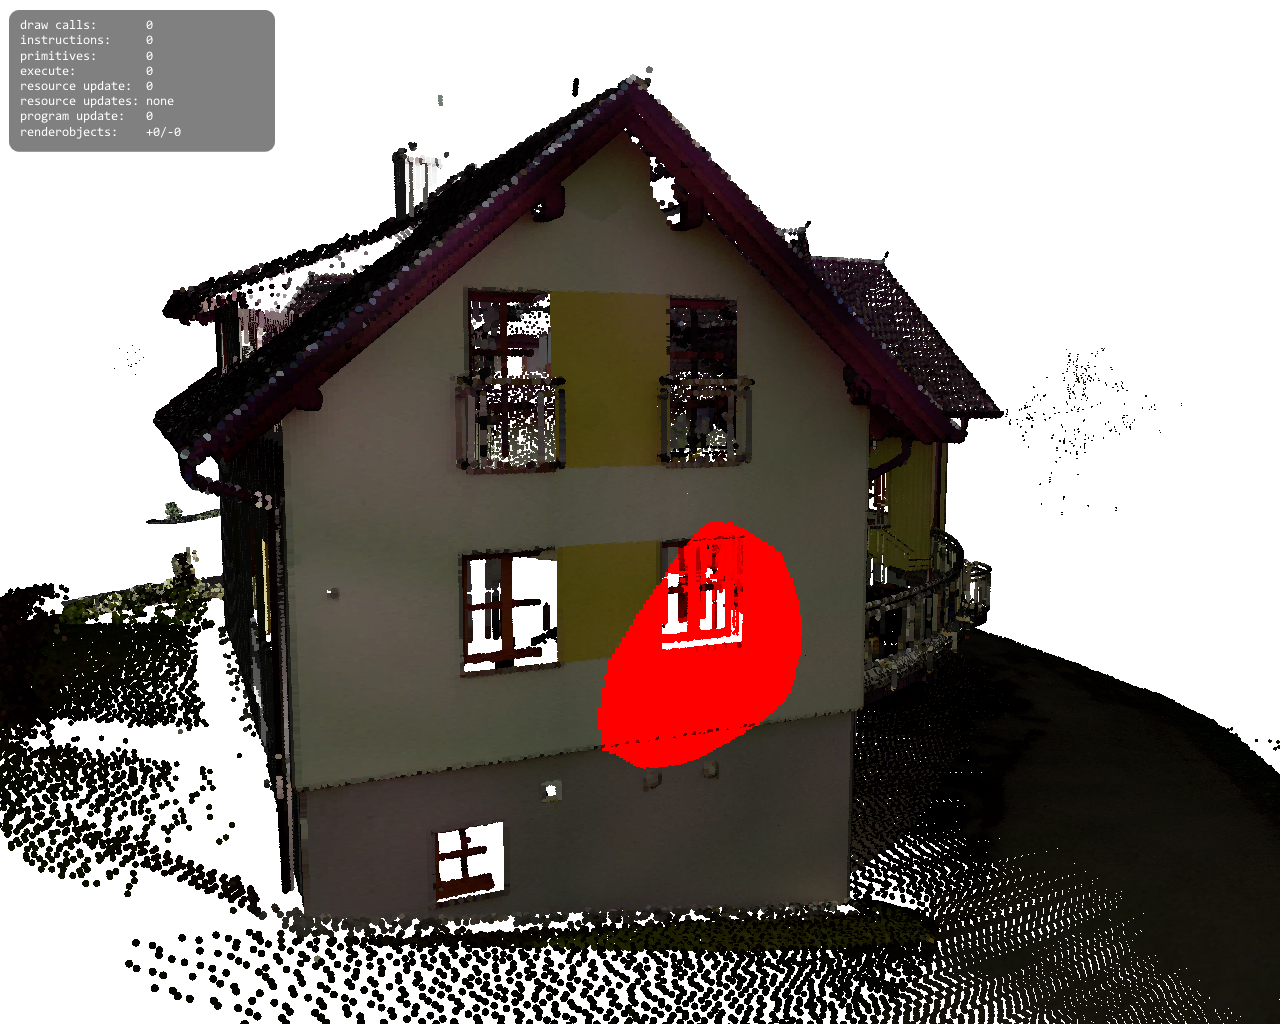
\includegraphics[width=0.5\textwidth]{Interactions/lasso2.png}%
  }\par\medskip        
\subcaptionbox{ \label{fig:lasso3}}{%
  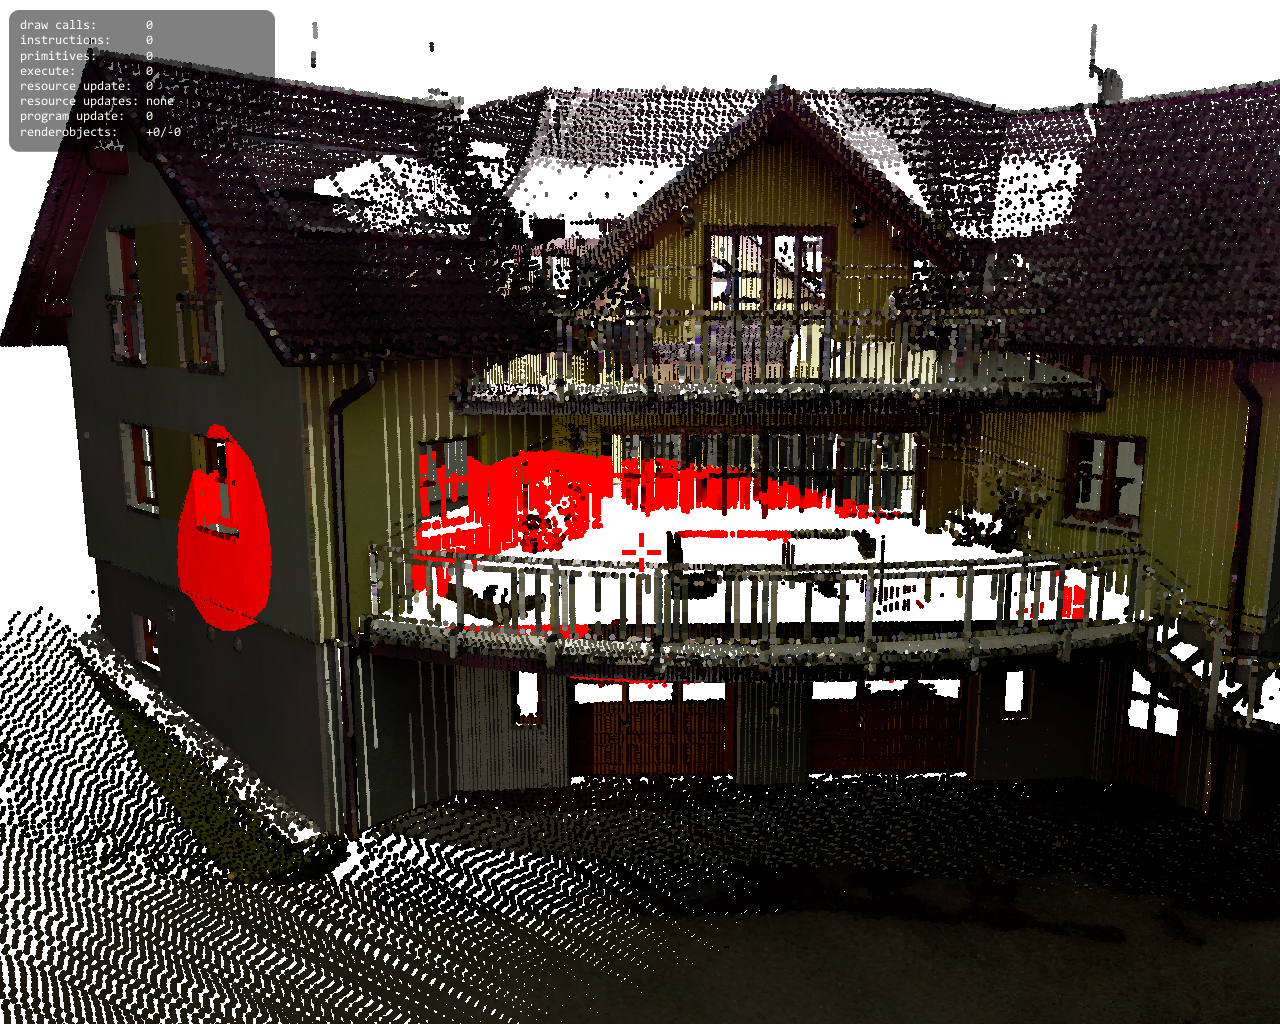
\includegraphics[width=0.5\textwidth]{Interactions/lasso3.png}%
  }
	
\caption{(a) - (c) show a lasso selection performed on a point cloud. In (a) the user draws a polygon onto the screen. In (b) the selected points are visualized in red. Figure (c) showcases the selection from a different angle. All points that are projected to the area of the polygon, are selected. This results in the unintentional selection of points that are obscured by objects in the foreground.}
\label{fig:lasso}
\end{figure}


Figure \ref{fig:lasso} shows a lasso selection performed on a point cloud. The user draws a polygon onto the screen. The selected points are highlighted in red. When changing the view, selected points that where occluded when drawing the lasso, appear. The user must control the selection distance by hand in order to minimize this effect. However, the in order to solve the task of only selecting points on the wall, further lasso selections must be used to remove points from the selection that where selected unintentionally. 





\subsection{Shape-Assisted Region Selection}
\section{Shape-Assisted Local Level-of-Detail Increase}

\chapter{Out-of-core Octree}
\label{chap:octree}

The term \textit{out of core} is used to describe the management of datasets whose size exceeds the available system memory. In this thesis, an out-of-core data structure is needed to handle large-scale point clouds efficiently. Section \ref{sec:octree_overview} gives an overview in the data structure that is used in this thesis, Section \ref{sec:octree_ooc} discusses the out-of-core organization of the octree. Section \ref{sec:octree_post} gives insight on the post-processing of the point cloud once the octree is created. Section \ref{sec:octree_culling} describes the task of creating a smaller representation of the octree that can be rendered efficiently. Section \ref{sec:octree_memory} concludes this chapter with a brief discussion about the memory consumption of this solution. 


\section{Overview}
\label{sec:octree_overview}

An octree is a hierarchical data structure in which each node represents a spatial region defined by a three-dimensional bounding box. If the decision is made to split a node, eight children are created, each representing an octant of the parent's bounding box. Due to the spatial subdivision properties, an octree is a popular data structure for storing point clouds. The spatial subdivision is a characteristic that is shared amongst almost all octree implementations. A characteristic that varies in each application is the composition of the content of octree's nodes. Various approaches exist that store point clouds in different ways. 

If an octree node is partitioned, the node's point set is distributed among the child nodes and the original node. 
Instant Points \cite{wimmer2006instant} keeps a small subset of points in the original node and distributes the remaining points according to the spatial position. This way, no points are duplicated, making it very memory efficient. 
Wand et al. \cite{wand2007interactive} distribute the entire point set among the node's children. The original node keeps an averaged subset of points. Thus, a multi-resolution representation of the point cloud is created at the cost of a larger memory footprint. 

This thesis uses an octree with a structure similar to that of Wand et al. If a node is partitioned, the point set is divided amongst its child nodes. A random subset of the original points is kept in the original node. Thus an efficient level-of-detail representation of the point cloud is created. 
The reason for not using the averaged subset is that the octree is tailored towards shape detection. This processing step is intended to be performed on original data. Moreover, for shape detection, each node is viewed as self-contained, such that no points from predecessor nodes are needed to represent the point cloud for this region and resolution entirely. This self-containment property is the reason why Wand et al.'s approach combined with the proposed subsampling technique is favored above an Instant-Points-like system. 

\par

Numerous decision rules exist that determine whether a node is split or not. A node is partitioned if the point count exceeds a threshold $n$. In this thesis, a decision based on the number of points in a node is favored as it keeps the number of points per node consistent.
Having a consistent number of points allows the variation in loading time and data size to be kept low. With nodes of consistent size, the runtime of procedures that are directly affected by the number of points for different nodes is similar as well. Therefore, such methods can be used in a context where immediate feedback is useful, such as user interactions, since the execution time can be estimated. In this thesis, a split threshold of 5000 points in a node is chosen. 


\section{Out-of-core Functionalities}
\label{sec:octree_ooc}
This thesis utilizes an out-of-core octree that stores each node's information and content separately. A \textit{chunk} describes a coherent portion of data that is stored in the cache file. Each octree node is built so that the node's information and node's content is stored in separate chunks. If an octree node is loaded into memory, the content of the node (i.e., the point set) remains on the hard drive. Only on explicit access, the point-set data is loaded into memory. Child nodes are stored as chunks as well. This interleaved structure of chunks allows for the minimal memory consumption for nodes, whose content is not needed directly. For example, bounding-box intersections can be calculated without the need of loading the point set into memory. Figure \ref{fig:out-of-core} shows the interleaved chunk structure of the out-of-core octree. Loading data into memory can only be done as long as free memory is available. Unused chunks of data are removed from memory after not being accessed for a distinct amount of time.

\begin{figure}
    \centering
    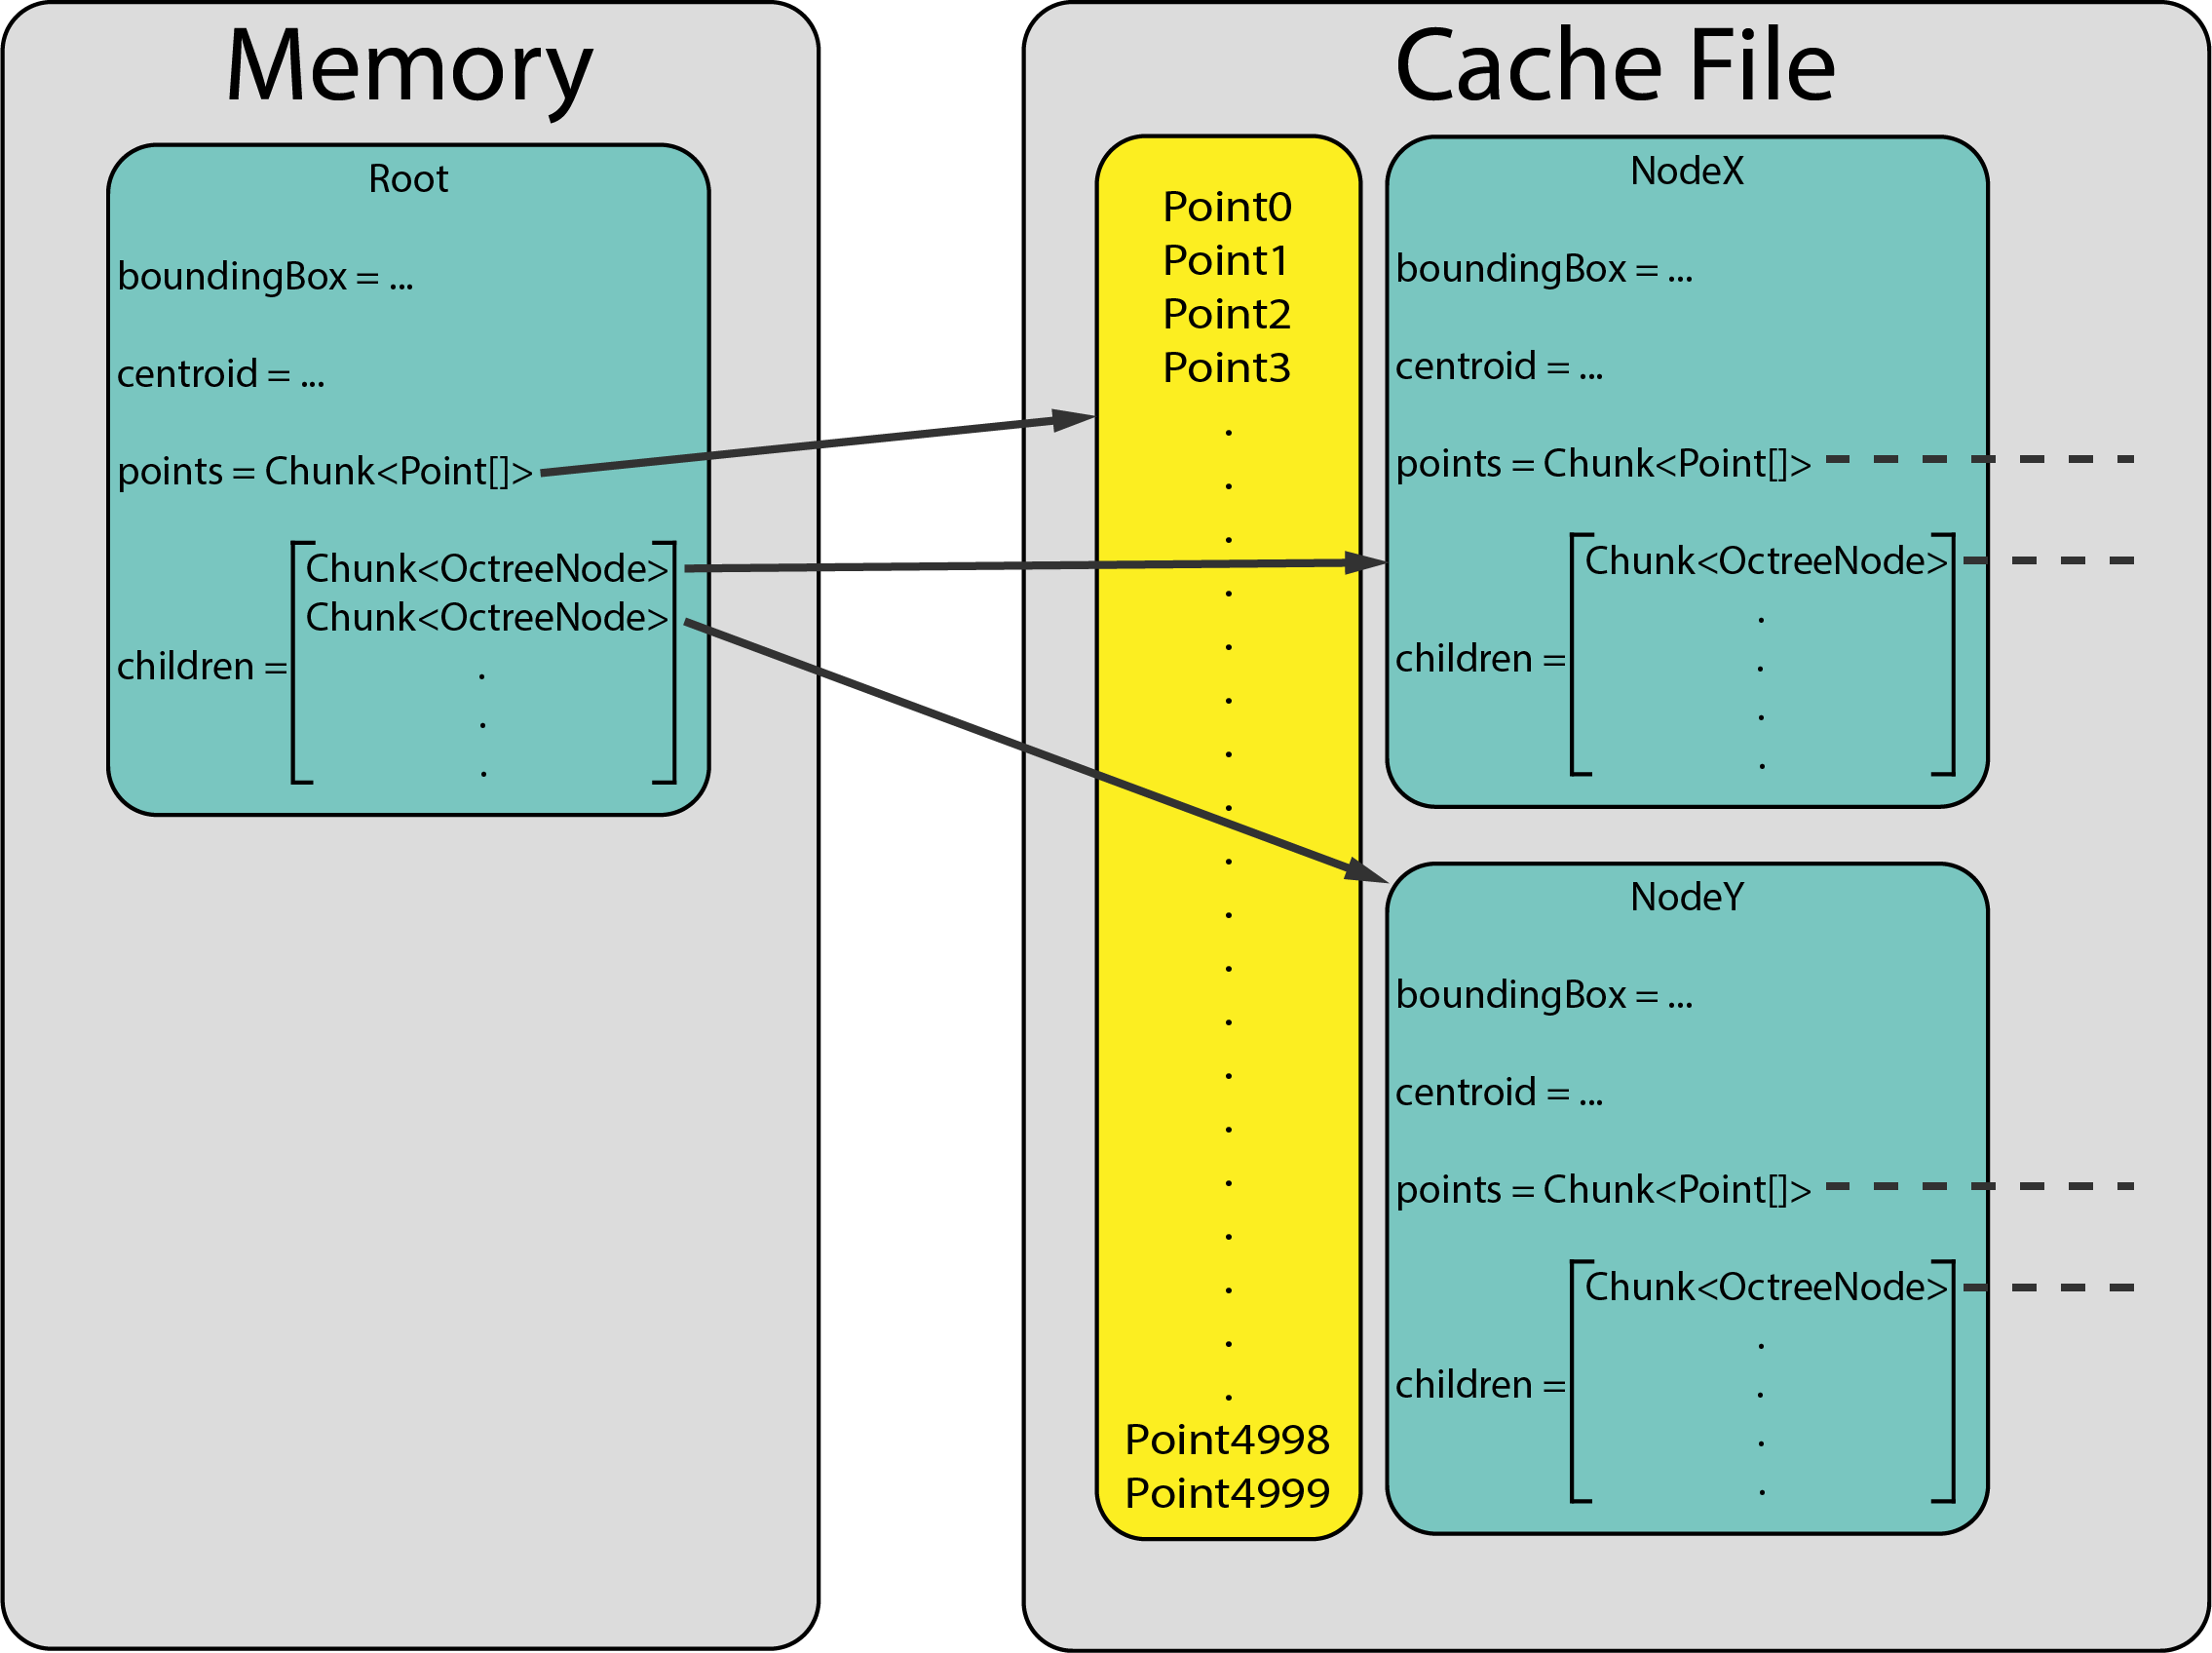
\includegraphics[width=0.5\textwidth]{Octree/out-of-core.png}
    \caption[Graphic describing the out-of-core structure of the octree]
        {This figure showcases the out-of-core structure of an octree with only the root node in the system memory(left). The point set remains in the cache file, as well as the node's children. Only necessary information, such as the node's bounding box and centroid are loaded into memory together with the node itself.}
    \label{fig:out-of-core}
\end{figure}


\section{Octree Postprocessing}
\label{sec:octree_post}
Point clouds often only contain information on position and color and lack distinct geometric features such as normal vectors. Normal vectors are significant for shape detection as they introduce information on the local curvature to the point cloud. After the octree build process is completed, additional properties are computed to enrich the dataset with more specific information. 


\subsection{rkd-Tree}

An rkd-tree \cite{tobler2011rkd} is an efficient data structure to perform fast n-nearest neighbor searches in static data sets. While the octree partitions the space into somewhat small regions, the rkd-tree further bisects the point set along the axes of the point space until only a single point is contained in each section. The rkd-tree improves the kd-tree by Friedman and Bentley \cite{friedman1975algorithm} by storing the radius of the sphere containing all points from the node's left and right subtrees. Thus, an early exclusion test with the sphere improves the performance of point queries. Instead of using a pointer-based binary search tree, the point array is rearranged so that the split point (i.e., median) for each bisection is located between the values of the one subtree and the values of the other subtree. Therefore, for each point in the array, only the index of the split dimension needs to be stored. 


\subsection{Normals}

For lighting and shape detection, each point must possess a normal vector. The local neighborhood determines a point's normal. Using the node's rkd-tree, a $k$-nearest-neighbor search is performed to retrieve the $k$ closest neighbors. Principal Component Analysis \cite{jolliffe2002principal} is used to fit a plane into the neighborhood. The plane's normal is defined by the eigenvector with the smallest eigenvalue. The plane's normal vector is used as the point's normal.


\subsection{Centroid}

The centroid of a node provides an indicator of the distribution of points in the octree node. The centroid is used as a target for the camera to focus on the presumably most dense part of the point cloud. 


\subsection{Density}

The density describes the average distance between a point and its nearest neighbor. The density increases with higher level-of-detail since more points are contained in a smaller region. To find the nearest neighbor, the node's rkd-tree is used again.


\section{Octree Culling}
\label{sec:octree_culling}

As a point cloud contains more data than the GPU can render in reasonable time, only points from those nodes are drawn that contribute to the currently viewed scene. The result of the culling operation is a new octree that contains only nodes that are currently rendered. The culled octree uses the same cached point information as the original octree. Thus, memory consumption is kept minimal. 

\par

A simple yet powerful culling heuristic is view-frustum culling. Nodes that are outside of the view frustum are discarded. By using view-frustum culling, whole branches of the octree are removed. The remaining branches are still too large to be rendered completely. A level-of-detail decision function determines whether or not a node should be rendered. Depending on the node's volume and distance to the near plane, a decision is made if the node should be rendered or not. 

\par

The heuristic culls hierarchically, meaning that if a parent is excluded, its children are as well. Thus, entire branches can be removed from the octree efficiently by only checking the parent node. If the octree is culled purely for rendering purposes, it is sufficient to collect the visible nodes in a set and use it for rendering. However, since interaction and processing tasks are performed on the viewed data, the hierarchical structure is kept intact. The intact hierarchy allows these tasks to exploit the octree structure and exclude entire branches of the culled octree with little computational cost. 


\section{Memory Consumption and Performance}
\label{sec:octree_memory}

The number of nodes from one level of detail to the next increases by the factor of $8$ (assuming that the octree is balanced and subdivided evenly). In reverse, when starting from the leaves, the number of nodes decreases by the factor of $\frac{1}{8}$. The upper bound of the relative size of the data stored in the entire octree is calculated from the geometric series: 


$$s = 1 + \frac{1}{8} + \frac{1}{64} + \frac{1}{512} + ... = \sum_{i = 0}^{\infty}{\frac{1}{8^i}} = \frac{8}{7}$$


To create the level-of-detail representation of the point cloud the size of the cache file and the number of stored points is increased by the factor of $\frac{8}{7}$. 

\par

All nodes from the culled octree are rendered, resulting in the multiple drawing of subsampled points from nodes with a lower level of detail. The previous calculations can be applied to estimate the overdraw when rendering the point cloud. The multiply drawn points account for $\sim$12\% of the entire point budget. The overdraw could be reduced by not drawing nodes whose children are already drawn. However, the current implementation lacks this improvement. 

\chapter{Shape Detection}
\label{chap:shapeDetection}


\section{Overview}

This thesis utilizes shape detection to automatically detect primitive shapes for small parts of the point cloud at a time. It is designed in such a way that the user receives immediate feedback of local geometry for the region under the mouse cursor. The approach utilizes an automated shape detection algorithm that is capable of detecting different types of primitive shapes. This algorithm is designed to find shapes in point clouds that consist of several million points within minutes. However, when looking at the performance for smaller samples, results can be achieved at interactive time rates. Section \ref{sec:schnabel} describes the shape detection algorithm in detail. 
\\

Before using the detected shapes for rendering or interactions, the shapes must be postprocesssed. Since some of the shapes are of infinite size, they need to be refitted to encapsulate the corresponding support points and create a minimal boundary. Section \ref{sec:Refitting} describes this task. 
\\

Section \ref{sec:shapeMatching} proposes a set of heuristics to determine if detected primitive shapes originate from the same geometric structure. Section \ref{sec:shapeClustering} explains the usage of this heuristics in order to create larger, homogeneous cluster of shapes, used for interactions. 


\section{Efficient RANSAC for Point-Cloud Shape Detection}
\label{sec:schnabel}

The section gives a brief overview over the algorithm used to detect primitive shapes. 
Schnabel et al. \cite{schnabel-2007-efficient} propose an automated way to detect simple primitive shapes in unstructured point clouds. The point cloud is decomposed into a set of shapes and a set of unused points. The algorithm supports detection of planes, spheres, cylinders, cones, and tori. 

\textbf{RAN}dom \textbf{SA}mpling \textbf{C}onsens (RANSAC) was first discussed by Fischler and Bolles \cite{fischler1981random} as a paradigm for model fitting for image analysis and automated cartography. However, this approach can be generalized for points with an origin other than images. The shape detection utilizes RANSAC to repeatedly take a minimal set of points to build a primitive shape $\Psi$ and checks if the points in the region roughly follow the curvature of the shape. 

\subsection{Minimal sets}

A minimal set describes the set of points that are needed to construct a candidate shape. 
For each type of shape, the following rule applies: A shape is only considered as candidate shape if all points from the minimal set are within a distance $\epsilon$ to the shape and the normal does not deviate from the shape's normal by more than an angle $\alpha$. 

\begin{itemize}
    \item \textbf{Plane}: A plane is constructed from three points $p_0, p_1, p_2$ whose normals do deviate from the plane's normal less than the angle $\alpha$. 
    
    \item \textbf{Sphere}: A sphere is fully defined by two points $p_0, p_1$ with corresponding normal vectors $n_0, n_1$. The center $c$ of the sphere is defined by the midpoint shortest line segment between the parametric lines $p_0 + tn_0$ and $p_1 + sn_1$. The radius is constructed by averaging the distance of $p_0$ and $p1$ to $c$.

    \item \textbf{Cylinder}:
    In order to create a cylinder, a minimal set of two points  $p_0, p_1$ with corresponding normal vectors $n_0, n_1$ is used. The direction $d$ of the axis is established by $d = n_0 \times n_1$. The origin $c$ of the cylinder is created by projecting the parametric lines $p_0 + tn_0$ and $p_1 + sn_1$ onto the plane $d \cdot x = 0$ and taking their intersection as origin $c$. The radius is the shortest distance between $p_0$ and the axis $c + ud$
    
    \item \textbf{Cone}:
    For simplicity, the minimal set for a cone consists of three points $p_0, p_1, p_2$, rather than two. For each point-normal pair, a plane is created. The intersection of the three planes defines the apex $c$. To describe the direction of the axis a plane is constructed from the points \{$c +  \frac{p_0 - c}{||p_0 - c||}$, $c +  \frac{p_1 - c}{||p_1 - c||}$, $c +  \frac{p_2 - c}{||p_2 - c||}$\}. The normal of this plane is the direction $d$ of the cone axis. The opening angle is given as $\omega = \frac{\sum_{i}^{max} (p_i - c)\cdot d}{3}$
    
    \item \textbf{Torus}:
    A minimal set of four points with normals is used, one more than theoretically necessary, However, this eases the computation.
    Two possible rotational axis are found by intersecting the four point-normal lines $p_i +  \lambda n_i$\cite{marshall2001robust}. For each axis, a full torus is estimated, and the torus is chosen that causes the smaller error in respect to the four points. The minor radius is found by projecting the points onto a plane that rotates around the axis. A circle is constructed using three points, whose radius is the minor radius of the torus. The major radius is given as the distance from the circle center to the axis. 


\end{itemize} 

\subsection{Score function}
\label{sec:scorefun}
To only use points that roughly follow the curvature of a candidate shape, only points within a distance $\epsilon$ are taken into account. Furthermore, each point must fulfill a score function to be considered a support point of the shape $\Psi$. 
The score function for each point consists of the following: 
\begin{itemize}
    \item The distance between the point and the shape must be smaller than $\epsilon$.
    \item The normal of the point must not deviate from the normal of the shape more than a given angle $\alpha$.
    \item Among all points that fulfill the previous two conditions, only the subset of points, which creates the largest connected component embedded in the shape,  is considered.
\end{itemize}

All points that are within a distance $\epsilon$ are taken into account. However, only those whose normals do not deviate from the normal of the shape more than a given angle $\alpha$ are considered support points. Additionally, the number of support points must exceed a threshold value $n$ for this shape to be valid. 


\subsection{Performance}

\begin{table}
    \centering
    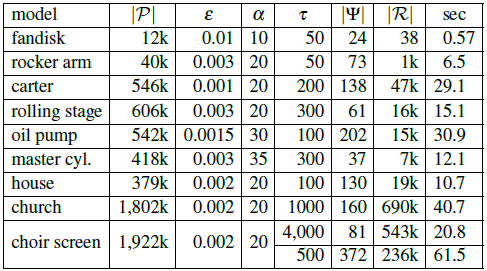
\includegraphics[width=0.7\textwidth]{Shape_Detection/schnabel-performance.png}
    \caption[Original statistics of the shape detection algorithm by Schabel et al.]{The original statistics by Schnabel et al. \cite{schnabel-2007-efficient} on processed models. $\epsilon$ is given as ration of maximum bounding box with. Results have been averaged over 5 runs and rounded.}
    \label{table:schnabel_performance}
\end{table}

Table \ref{table:schnabel_performance} describes the statistical results for different models. $|P|$ is the number of points, $\epsilon$ the distance threshold, $\alpha$ the maximum normals deviation, $\tau$ is the minimum number of support points, $\|Psi|$ the number of shapes found, $|R|$ the number of RANSAC iterations. It can be seen that for small a small number of points and weaker constraints the algorithm returns plausible results within a fraction of a second. We utilize this feature the detect shapes in our application for small regions at a time to give immediate feedback to the user. 


\section{Refitting}
\label{sec:Refitting}

Planes, cylinder, and cones are infinite shapes. Therefore, to use those shapes for rendering and interactions, it is necessary to create finite representations for each shape. Each shape comes with the corresponding set of support points that are used to refit the shape. Spheres and Tori are finite by definition. Therefore they do not require refitting. 


\subsection{Refitting planes}

Planes, however, are represented by a point and a vector. All support points are projected onto the plane, thus reducing the fitting problem to two dimensions. The procedure starts by computing the convex hull of the projected points with the help of Andrew's monotone chain 2d convex hull algorithm\cite{andrew1979another}. 
More complex polygons can be computed. However, for this purpose, a quad is sufficient. The quad is obtained by using the minimum-bounding-rectangle algorithm by Freeman\cite{freeman1975determining}. 


\subsection{Refitting cylinder}

A cylinder is defined by a center $p$, direction vector $v$ and a radius $r$. The height of the cylinder is chosen as the maximum distance between two support points on the axis of the cylinder. This is achieved by projecting all points onto the axis $a = p + vt$ of the cylinder, and select the points $p_{min}$, where $t$ is minimum and $p_{max}$, where $t$ is maximum. The distance $d$ between $p_{min}$ and $p_{max}$ is the height of the enclosing cylinder. The cylinder is refitted such that the new center is set to $p' = p_{min}$ and the $d$ is encoded in the length of the new direction vector:$v' = \frac{v}{|v|}d$. The radius stays the same. 


\subsection{Refitting cones}

A cone is defined by its apex $c$, axis direction $v$, and opening angle $\theta$. Similar to the cylinder, all support points are projected onto the axis and the points $p_{min}, p_{max}$, with minimum and maximum $t$, are selected. Since the apex of a cone is fixed, the range cannot be encoded using $c$ and $v$. The range is stored separately. Range checks are performed when rendering or interacting with cones. 


\section{Shape Detection Parameter Selection}
\label{sec:shapeDetectionParameterSelection}

This section briefly discusses the issue of selecting optimal parameters for the shape detection. The $\epsilon$ parameter creates an $\epsilon$-band that follows the curvature of the shape. All points within this $\epsilon$ band are considered to be candidates. The authors propose to use the point cloud's bounding boxes largest dimension times $0.1$ as $\epsilon$. However, using such a static parameter yields problems with extremely sparse regions and regions that are populated very densely. In this thesis, shape detection is performed dynamically on local regions of the point cloud at a time. The local density of an octree node is chosen as $\epsilon$. The density is calculated per octree node by averaging the distance of each point to its nearest neighbor. Thus, nodes that are populated more densely create finer geometry. 

The $\alpha$ parameter is used to determine the deviation between two directions. As the normals are the same at different level-of-detail, this parameter is static. We use an $\alpha$ value of $0.95$. 

The minimum number of support points per shape is set to $250$.
\section{Shape Matching}
\label{sec:shapeMatching}

Since shape detection if performed on multiple scales and shapes are extracted for small regions at a time, a heuristic is needed to determine if shapes from different nodes belong to the same structure. While on a low \textit{level-of-detail}, a wall may be contained by a single octree node, on a higher level, a node will only contain parts of the wall and multiple nodes contain primitive shapes that share this wall. This section presents a set of matching functions to determine if two shapes originate from the same geometry with a certain tolerance. Only shapes of the same type can be matching. Therefore it is not necessary to define functions to match e.g. a plane shape with a cone shape since the result will always be \verb|false|. 


\subsection{Elementary Matching Functions}
\label{sec:elementarMatchingFuns}

As the primitive shapes are represented by only a handful of parameters, it is sufficient to determine the matching of these parameters. Therefore, we firstly define elementary matching functions for numbers, vectors, positions, and axes. Since matching is an approximation of equality, each matching function's result is determined by comparing a computation result to a threshold $\epsilon$. If a matching function returns \verb|true|, the input values are considered to be matching. 

\begin{itemize}
    \item \textbf{Matching floats $f_1, f_2$}: 
        $$\frac{f_1}{f_2} \geq \epsilon, \textrm{ where } f_1 \leq f_2$$  
    \item \textbf{Matching vectors $v_1, v_2$}: 
        $$\frac{v_1}{|v_2|} \cdot \frac{v_2}{|v_2|} \geq \epsilon$$
    \item \textbf{Matching positions $p_1, p_2$}: 
        $$\sqrt{(p_1.x - p_2.x)^2 + (p_1.y - p2_y)^2 + (p1_z - p2_z)^2} \leq \epsilon$$
    \item \textbf{Matching axis $a_1, a_2$}: 
    \\
    An axis is defined by a start and end point. Let $p_{01},p_{02}$ be the start and end point of $a_1$ and $p_{11}, p_{12}$ the start and end point of $a_2$. Furthermore, let $v_1, v_2$ be the direction vectors of $a_1$ and $a_2$. The rays of the axes are denoted as $r_1 = p_{00} + sv_1$ and $r_2 = p_{10} + tv_2$. The closest distances for start and end point for each axis to the complementary ray are calculated. From those for values, the largest value $d$ is used for decision making. The matching decision is composed as follows: 
        $$\frac{v_1}{|v_2|} \cdot \frac{v_2}{|v_2|} \geq \epsilon_1 \land d \leq \epsilon_2$$
\end{itemize}


\subsection{Primitive Shape Matching Functions}
\label{sec:primitiveShapeMatchingFuns}

With the elementary matching functions defined in Section \ref{sec:elementarMatchingFuns}, it is easy to define matching functions for two primitive shapes based on the elementary matching functions:

\begin{itemize}
\item \textbf{Matching plane shapes}: 
A plane shape contains to a quad that encloses all support points. For distance computation, the plane is used, rather than the quad, since the origin of the plane shape is the plane. For each corner of each quad, the distance to the other plane is calculated. From those eight values, the largest distance $d$ is chosen. Two plane shapes are matching, if the planes' normal vectors are matching in retrospect to a threshold value $\epsilon_1$ and $d$ is smaller than or equal to a threshold value $\epsilon_2$.
\item \textbf{Matching cylinder shapes}: 
A cylinder consists of an axis and a radius. Two cylinder shapes are matching if radii and axes are matching. 
\item \textbf{Matching cone shapes}:
Cones consist of an axis, an apex, and an opening angle. Two cone shapes are matching if the axes, apexes and opening angles are matching. 
\item \textbf{Matching sphere shapes}: 
Two sphere shapes are matching if the center positions and the radii are matching. 
\item \textbf{Matching torus shapes}: 
A torus consists of a center position, an axis and a major and minor radius. Two torus shapes are matching if the center position, axes, major radii, and minor radii are matching. 
\end{itemize}

The matching result heavily depends on the chosen threshold values. Table \ref{tab:matchingThresholds} shows the $\epsilon$ values that are used for this implementation. Plane matching uses a custom heuristic that is not depicted in the table. For this heuristic, $\epsilon_2 = 0.05$ is chosen. Note that matching floats is a relative measure, whereas matching positions and axes uses world space distances as the threshold. Matching vectors uses the angle between the two vectors to calculate a matching. 

\begin{table}
\centering
\begin{tabular}{ r | r }
    Matching    & threshold values \\
    \hline
  Floats         & $\epsilon = 0.99$ \\
    Vectors     & $\epsilon = 0.95$ \\
  Positions & $\epsilon = 0.05$ \\ 
    Axis             & $\epsilon_2 = 0.05$, $\epsilon_1 = 0.95$ \\  

\end{tabular}
\caption{The different threshold values for parameter matching.}
\label{tab:matchingThresholds}
\end{table}


\section{Shape Clustering}
\label{sec:ShapeClustering}

With the user interaction in mind, it is not sufficient to interact with a single shape only. To determine the global extent of a primitive shape, more information is needed. Section \ref{sec:primitiveShapeMatchingFuns} describes a set of heuristics to determine if two primitive shapes originate from the same geometry. These heuristics are used in this section in order to create larger representations of a primitive shape. 
\textit{Shape Clustering} aims to find matching primitive shapes for a base shape and build a larger coherent cluster of primitive shapes over multiple level-of-details. The types of primitive shapes can be categorized as finite and infinite shapes. Spheres and tori are finite objects per definition, thus it is sufficient enough to find a set of matching primitive shapes to create a cluster. For infinite shapes, such as planes, cones, and cylinder, additional computations are needed in order to create a coherent shape cluster. Figure \ref{fig:cuboids} shows the case of two cuboids, whose front face share a plane. By only using the matching functions to create a cluster, both front faces are packed into the cluster, even tough there is a visible gap between them.

\begin{figure}
    \centering
    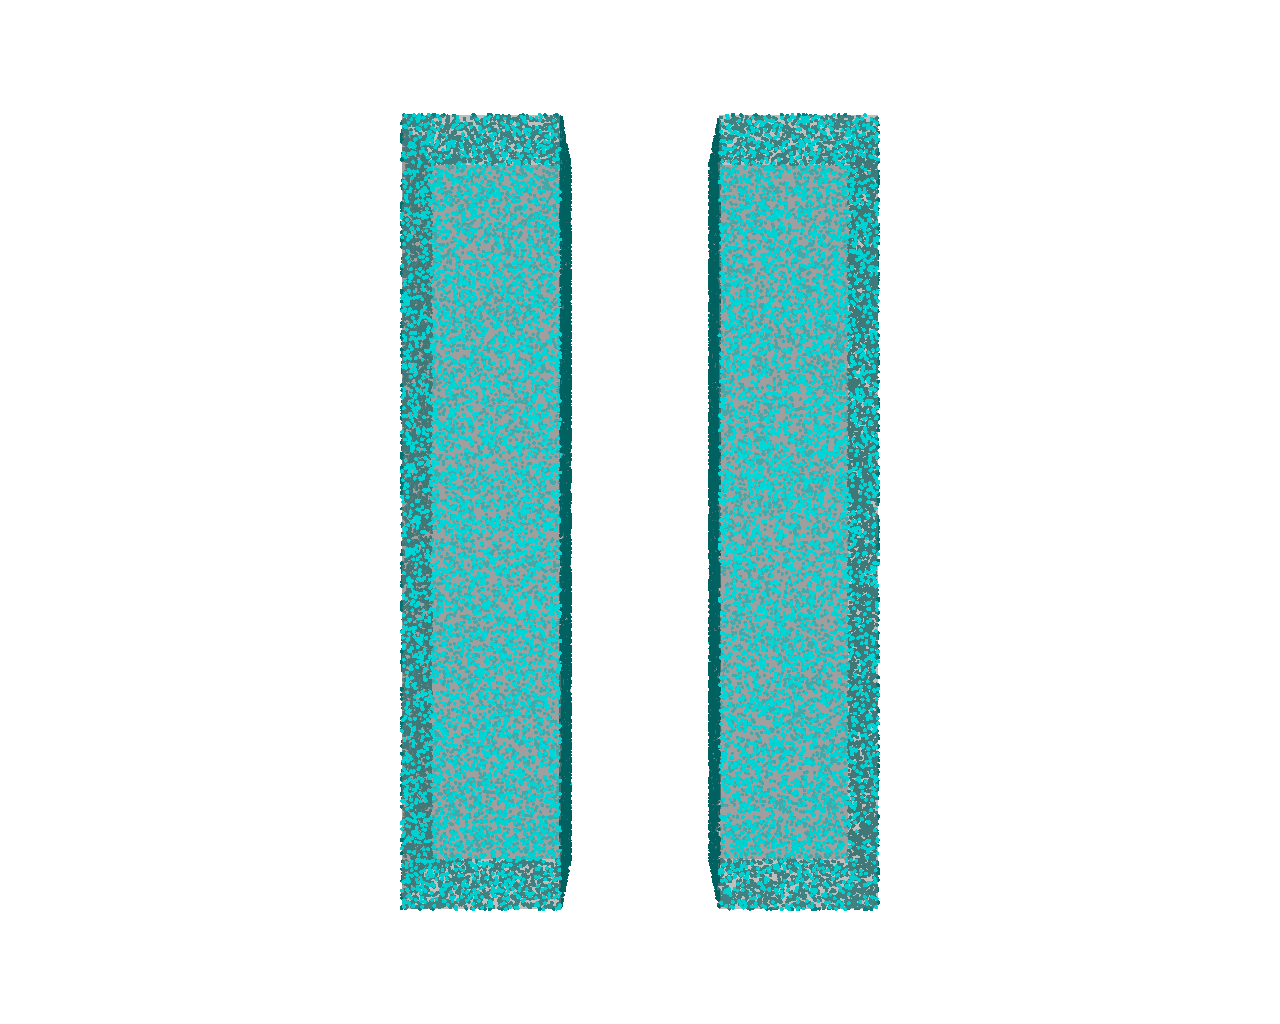
\includegraphics[width=0.8\textwidth]{Shape_Detection/cuboids.png}
    \caption{A generic point cloud of two cuboids. The detected planes are rendered in grey.}
    \label{fig:cuboids}
\end{figure}

Section \ref{sec:matchingSetBuilding} describes the procedure of finding matching shapes in the octree. For infinite shapes, an additional step is performed using a region-growing approach described in Section \ref{sec:regionGrowing}. 


\subsection{Building a set of matching primitive shapes}
\label{sec:matchingSetBuilding}

In order to find matching shapes, the octree is searched for primitive shapes that match the base shape. Only octree nodes are searched that are currently rendered, such that the cluster only consists of shapes that are present in the scene. Already, the cluster consists of shapes that share the same geometry as origin. For sphere and torus shapes, this step is sufficient enough to create a valid cluster, since both shapes are finite. 


\subsection{Graph-based Region Growing}
\label{sec:regionGrowing}

A cluster of shapes can be seen as an $\epsilon$-connected component from a larger graph. A complete graph is created using all matching shapes as vertices. In a complete graph, an edge exists for any pair of vertices. The weight of an edge is determined by a custom distance function for each primitive shape:

\begin{itemize}
    \item \textbf{Plane Shape}:         As a plane shape is bounded by a quad, the distance between two plane shapes is computed as the shortest distance between the two bounding quads.
    \item \textbf{Cylinder Shape}:    The shortest distance between two cylinder shapes is determined by the shortest distance of all pairs of start/end points of both cylinders. 
  \item \textbf{Cone Shape}:            The shortest distance between two cone shapes is determined by the shortest distance of all pairs of start/end points from both cones. 
\end{itemize}


A cluster is created by growing a region in a graph, adding only vertices that connect to the current region via an edge, whose weight is smaller than $\epsilon$. This creates a cluster of shapes, ensuring that the distance to the closest neighboring shape is at maximum $\epsilon$. 
\\
\begin{figure}
    \centering
    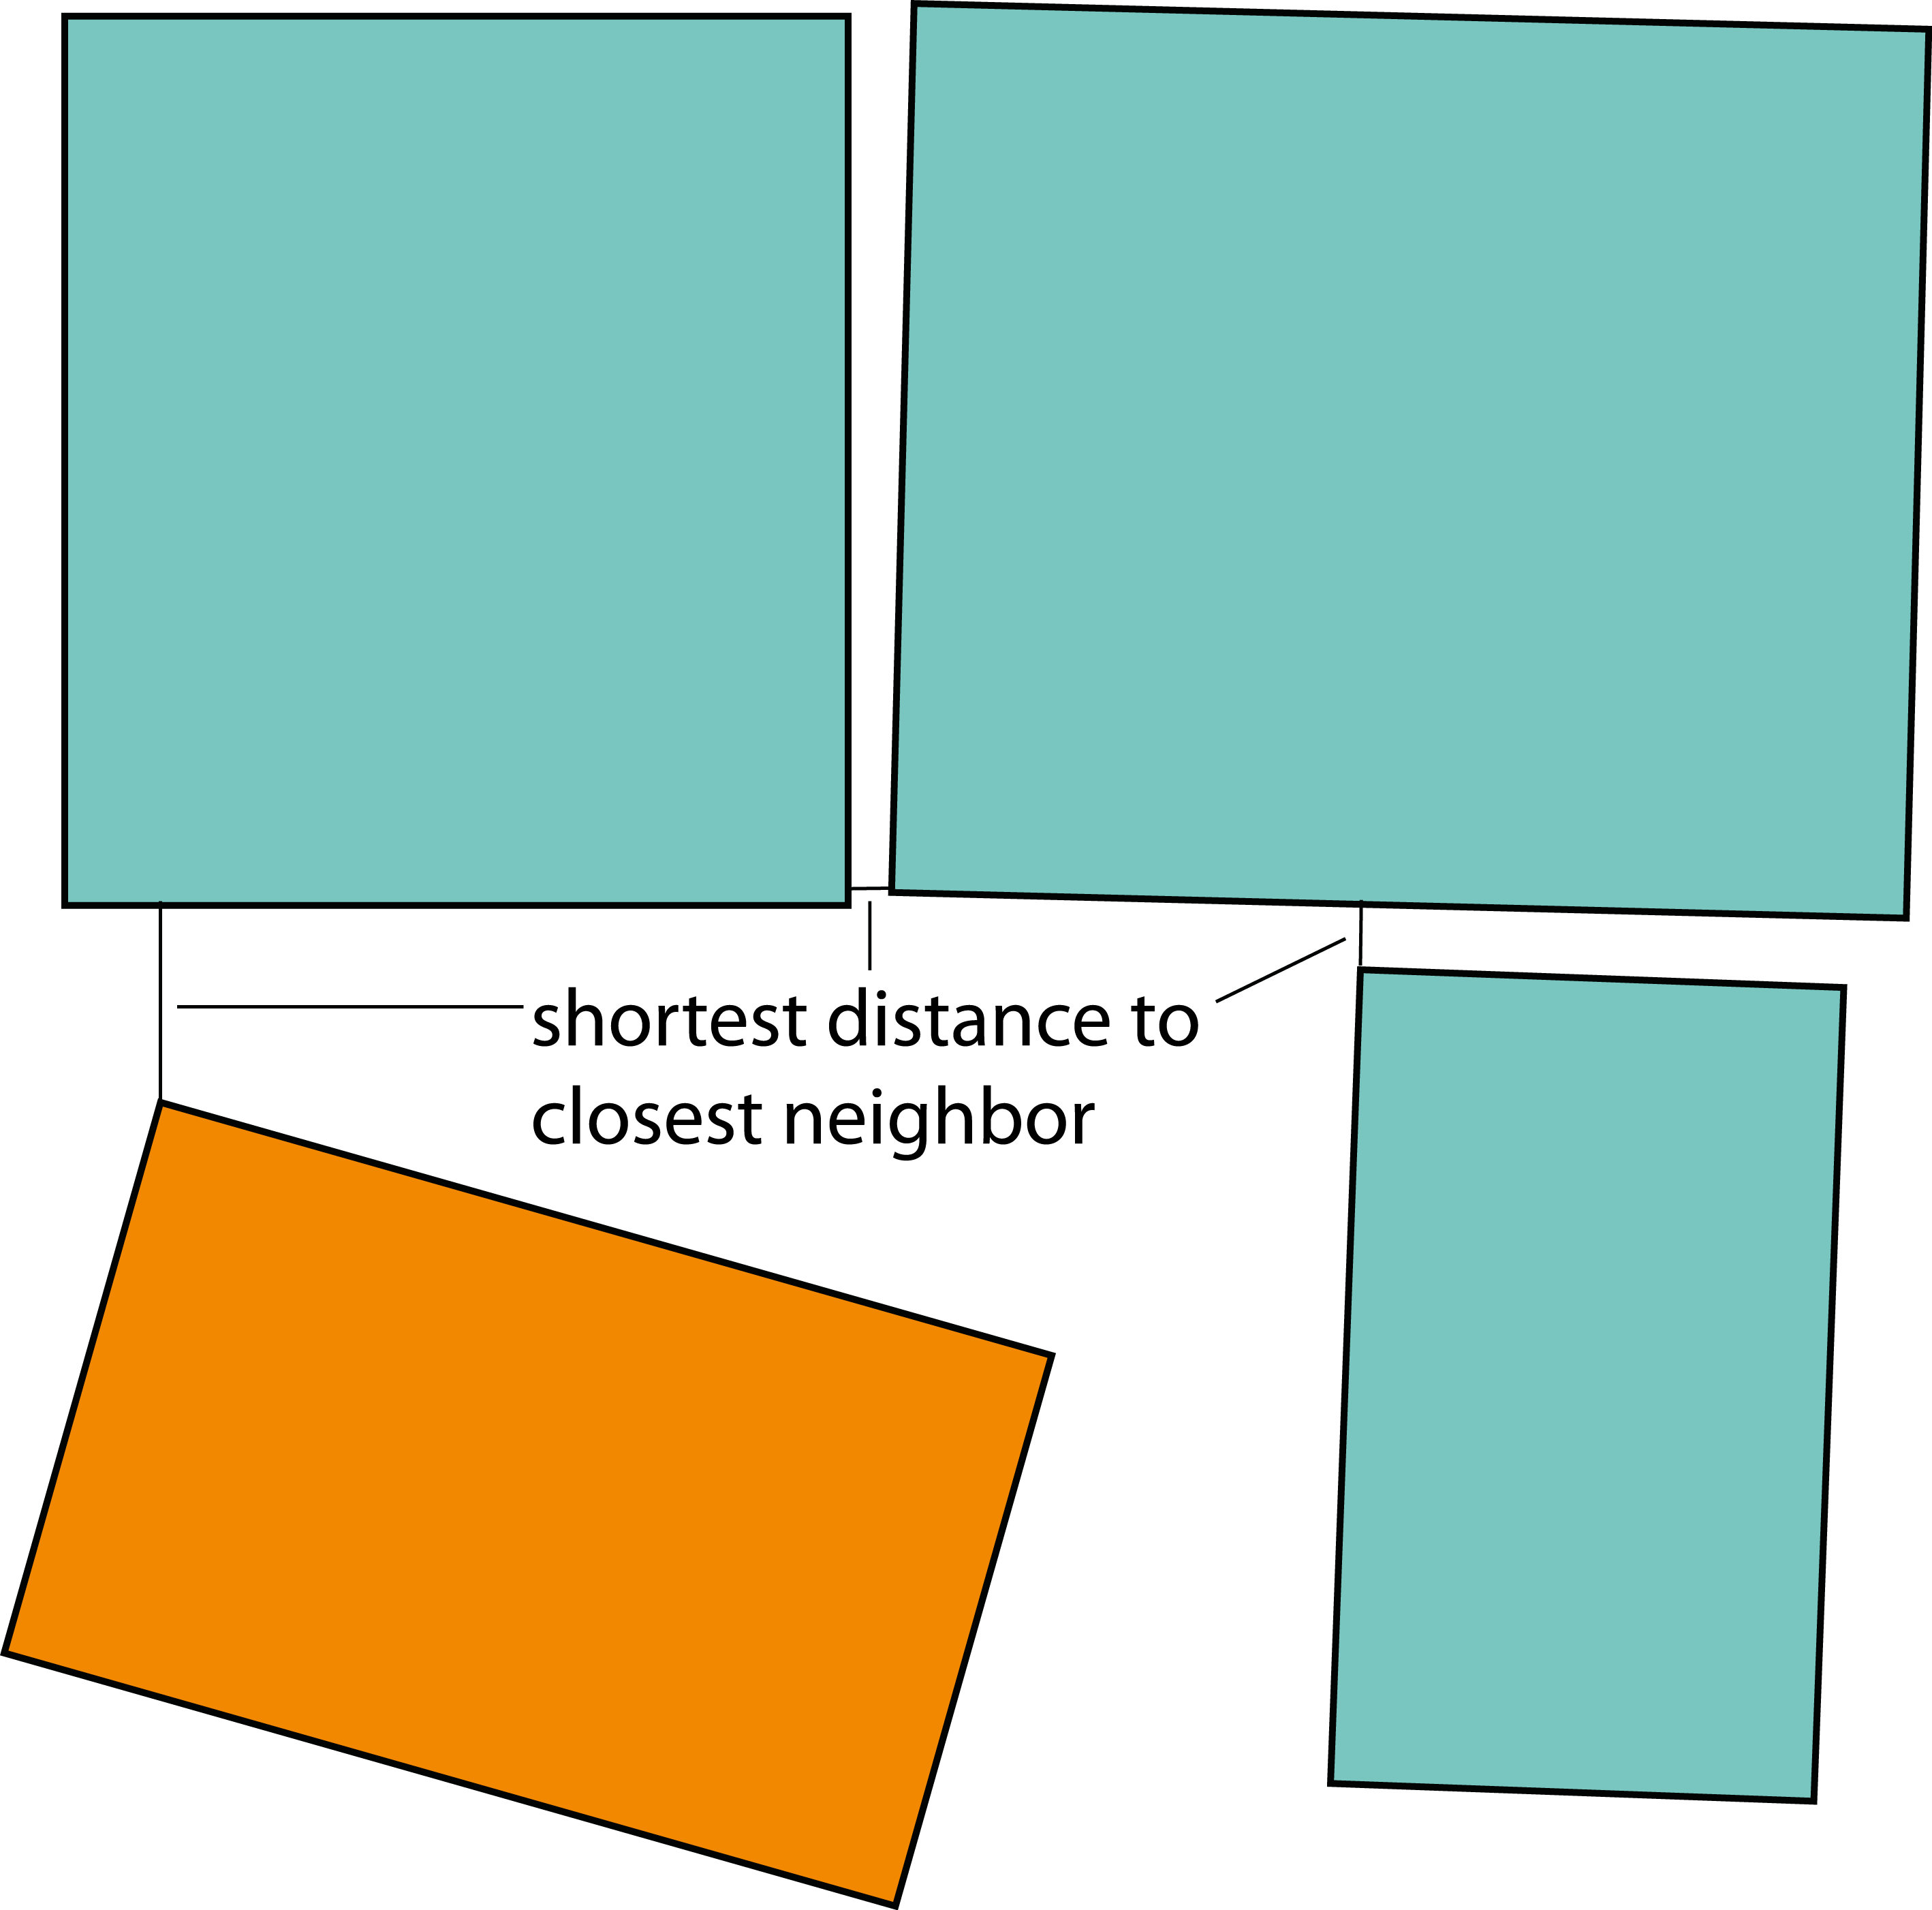
\includegraphics[width=0.5\textwidth]{Shape_Detection/regionGrowingPlanes.png}
    \caption{A cluster of plane shapes created by computing the $\epsilon$-connected component. Planes that belong to the cluster are colored in turquoise.}
    \label{fig:regionGrowingPlanes}
\end{figure}

Figure \ref{fig:regionGrowingPlanes} shows an exemplary illustration on region growing for plane shapes. The distance between two plane shapes is measured as the closest distance between the two bounding quads. 

\begin{figure}
\centering
\subcaptionbox{ \label{fig:regionGrowingCylinder}}{%
  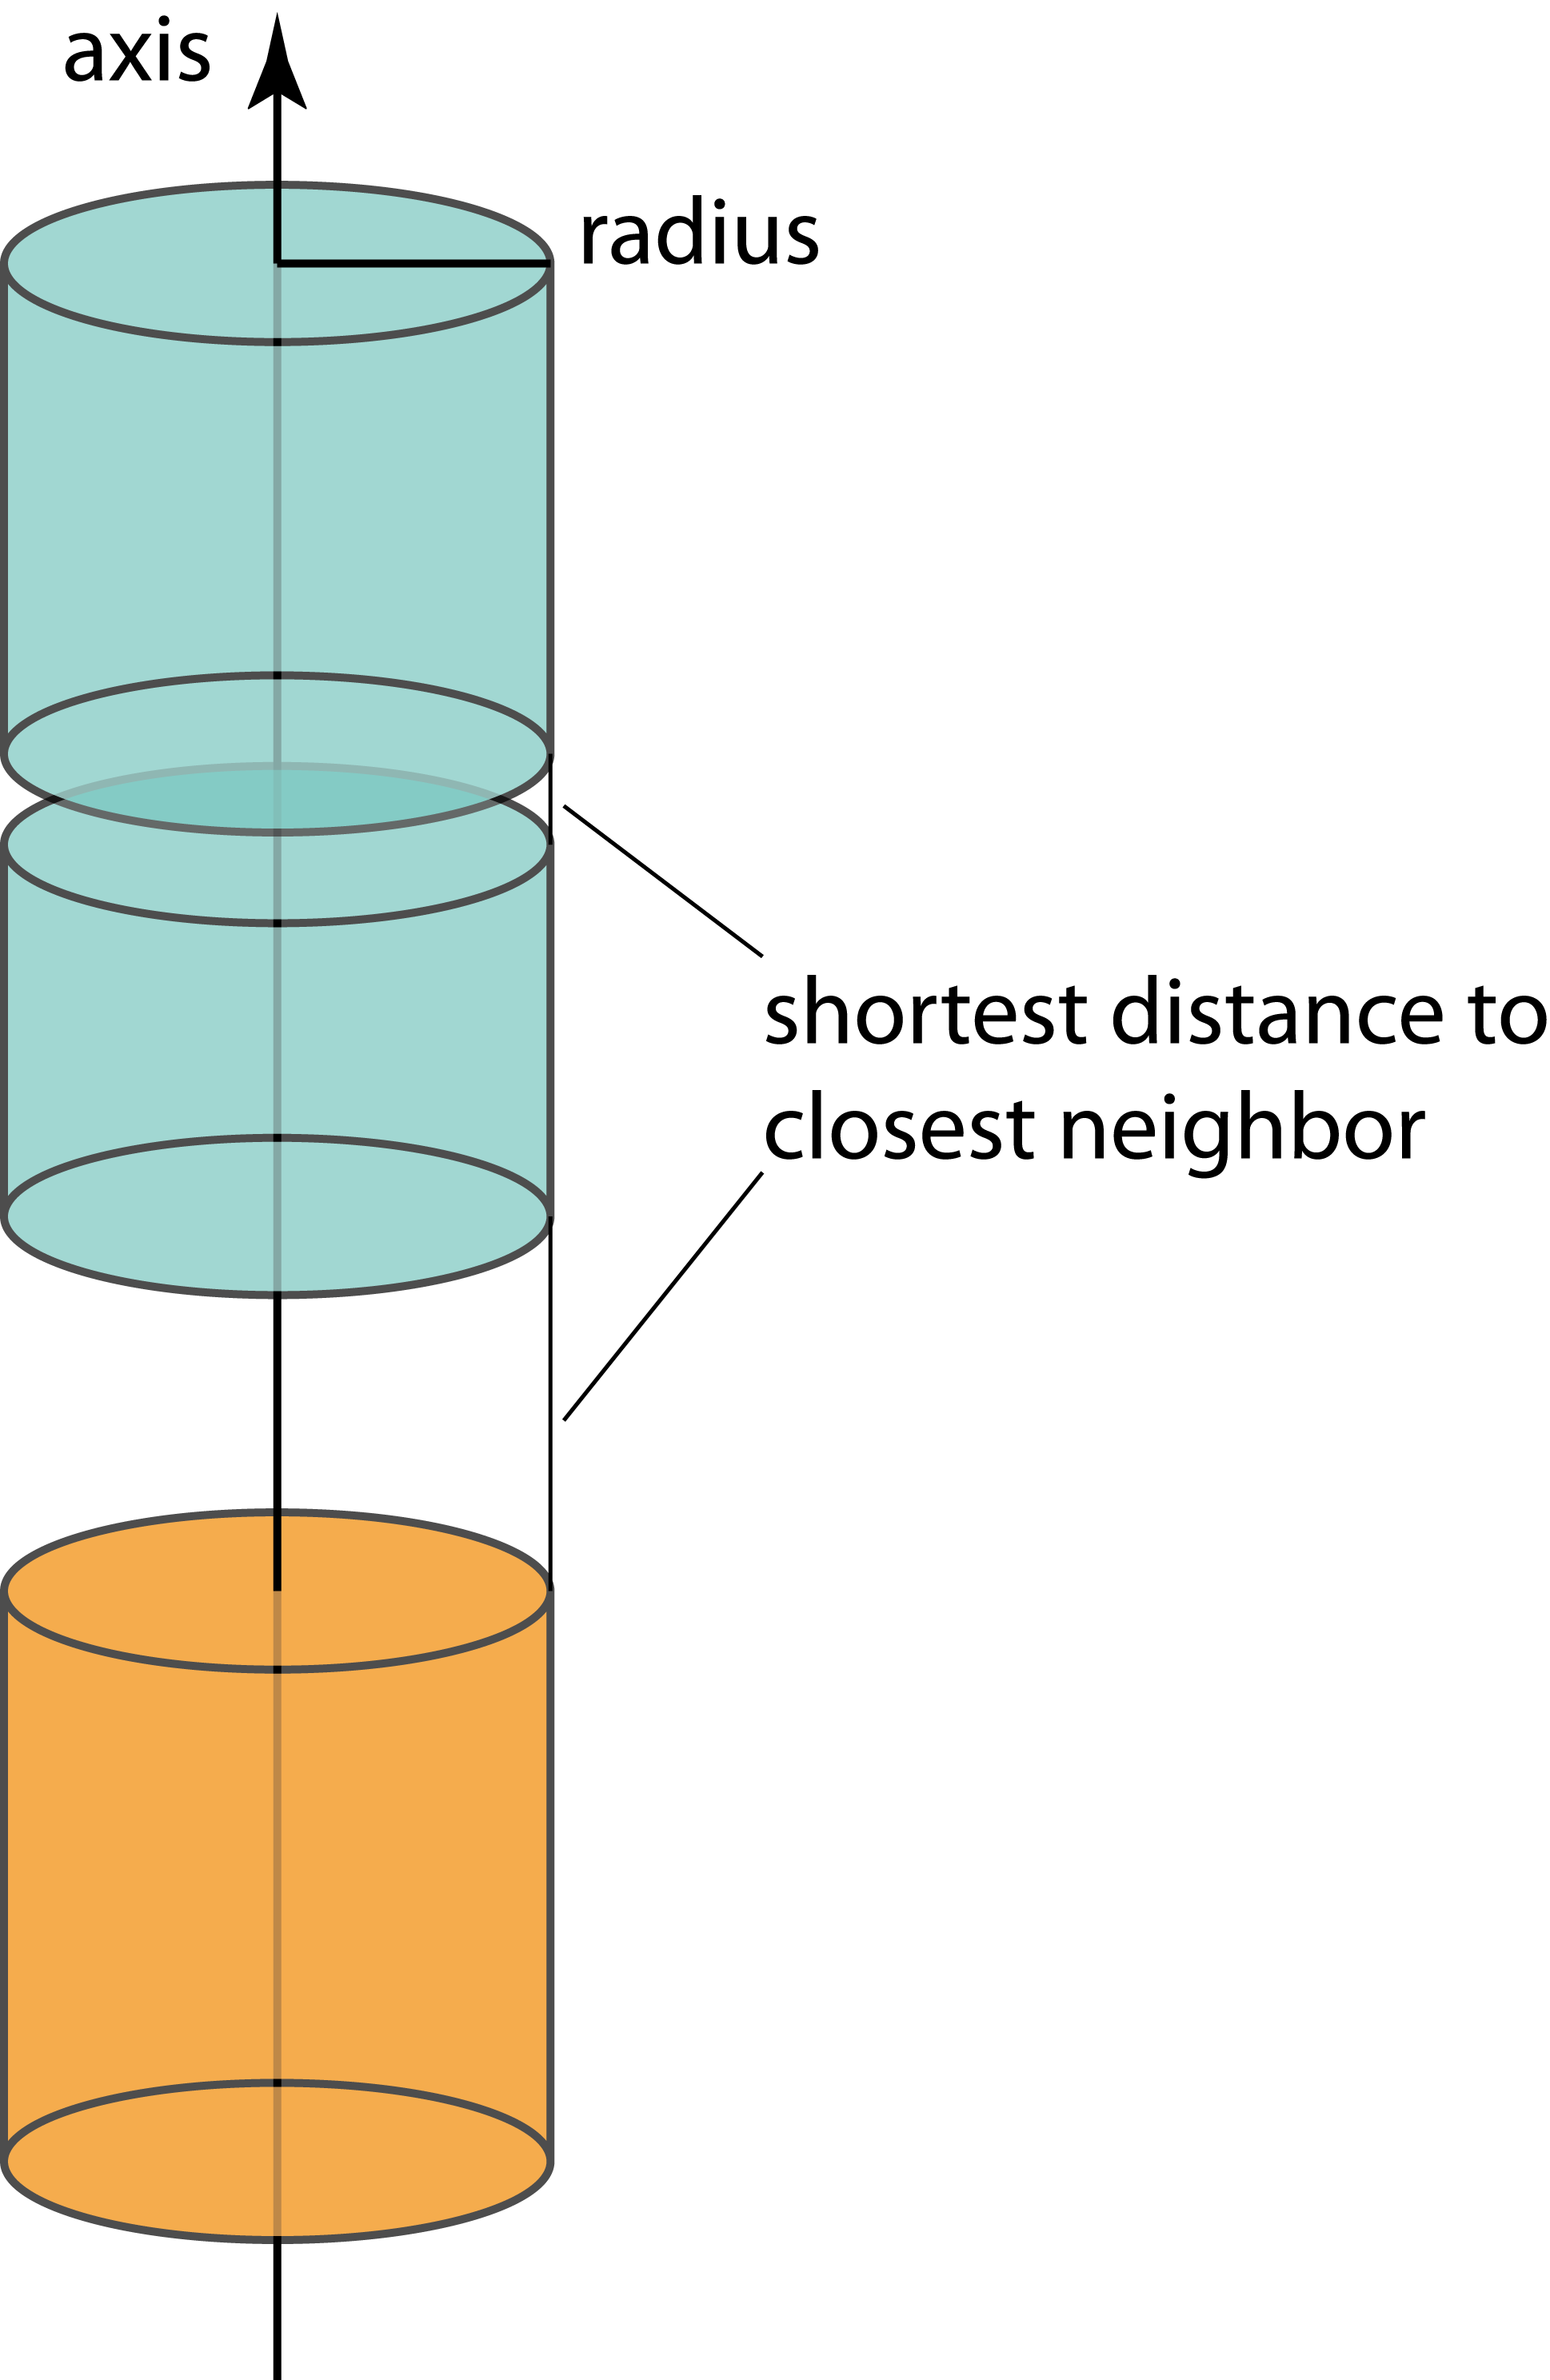
\includegraphics[width=0.3\textwidth]{Shape_Detection/regionGrowingCylinder.png}%7
  }
\subcaptionbox{ \label{fig:regionGrowingCone}}{%
  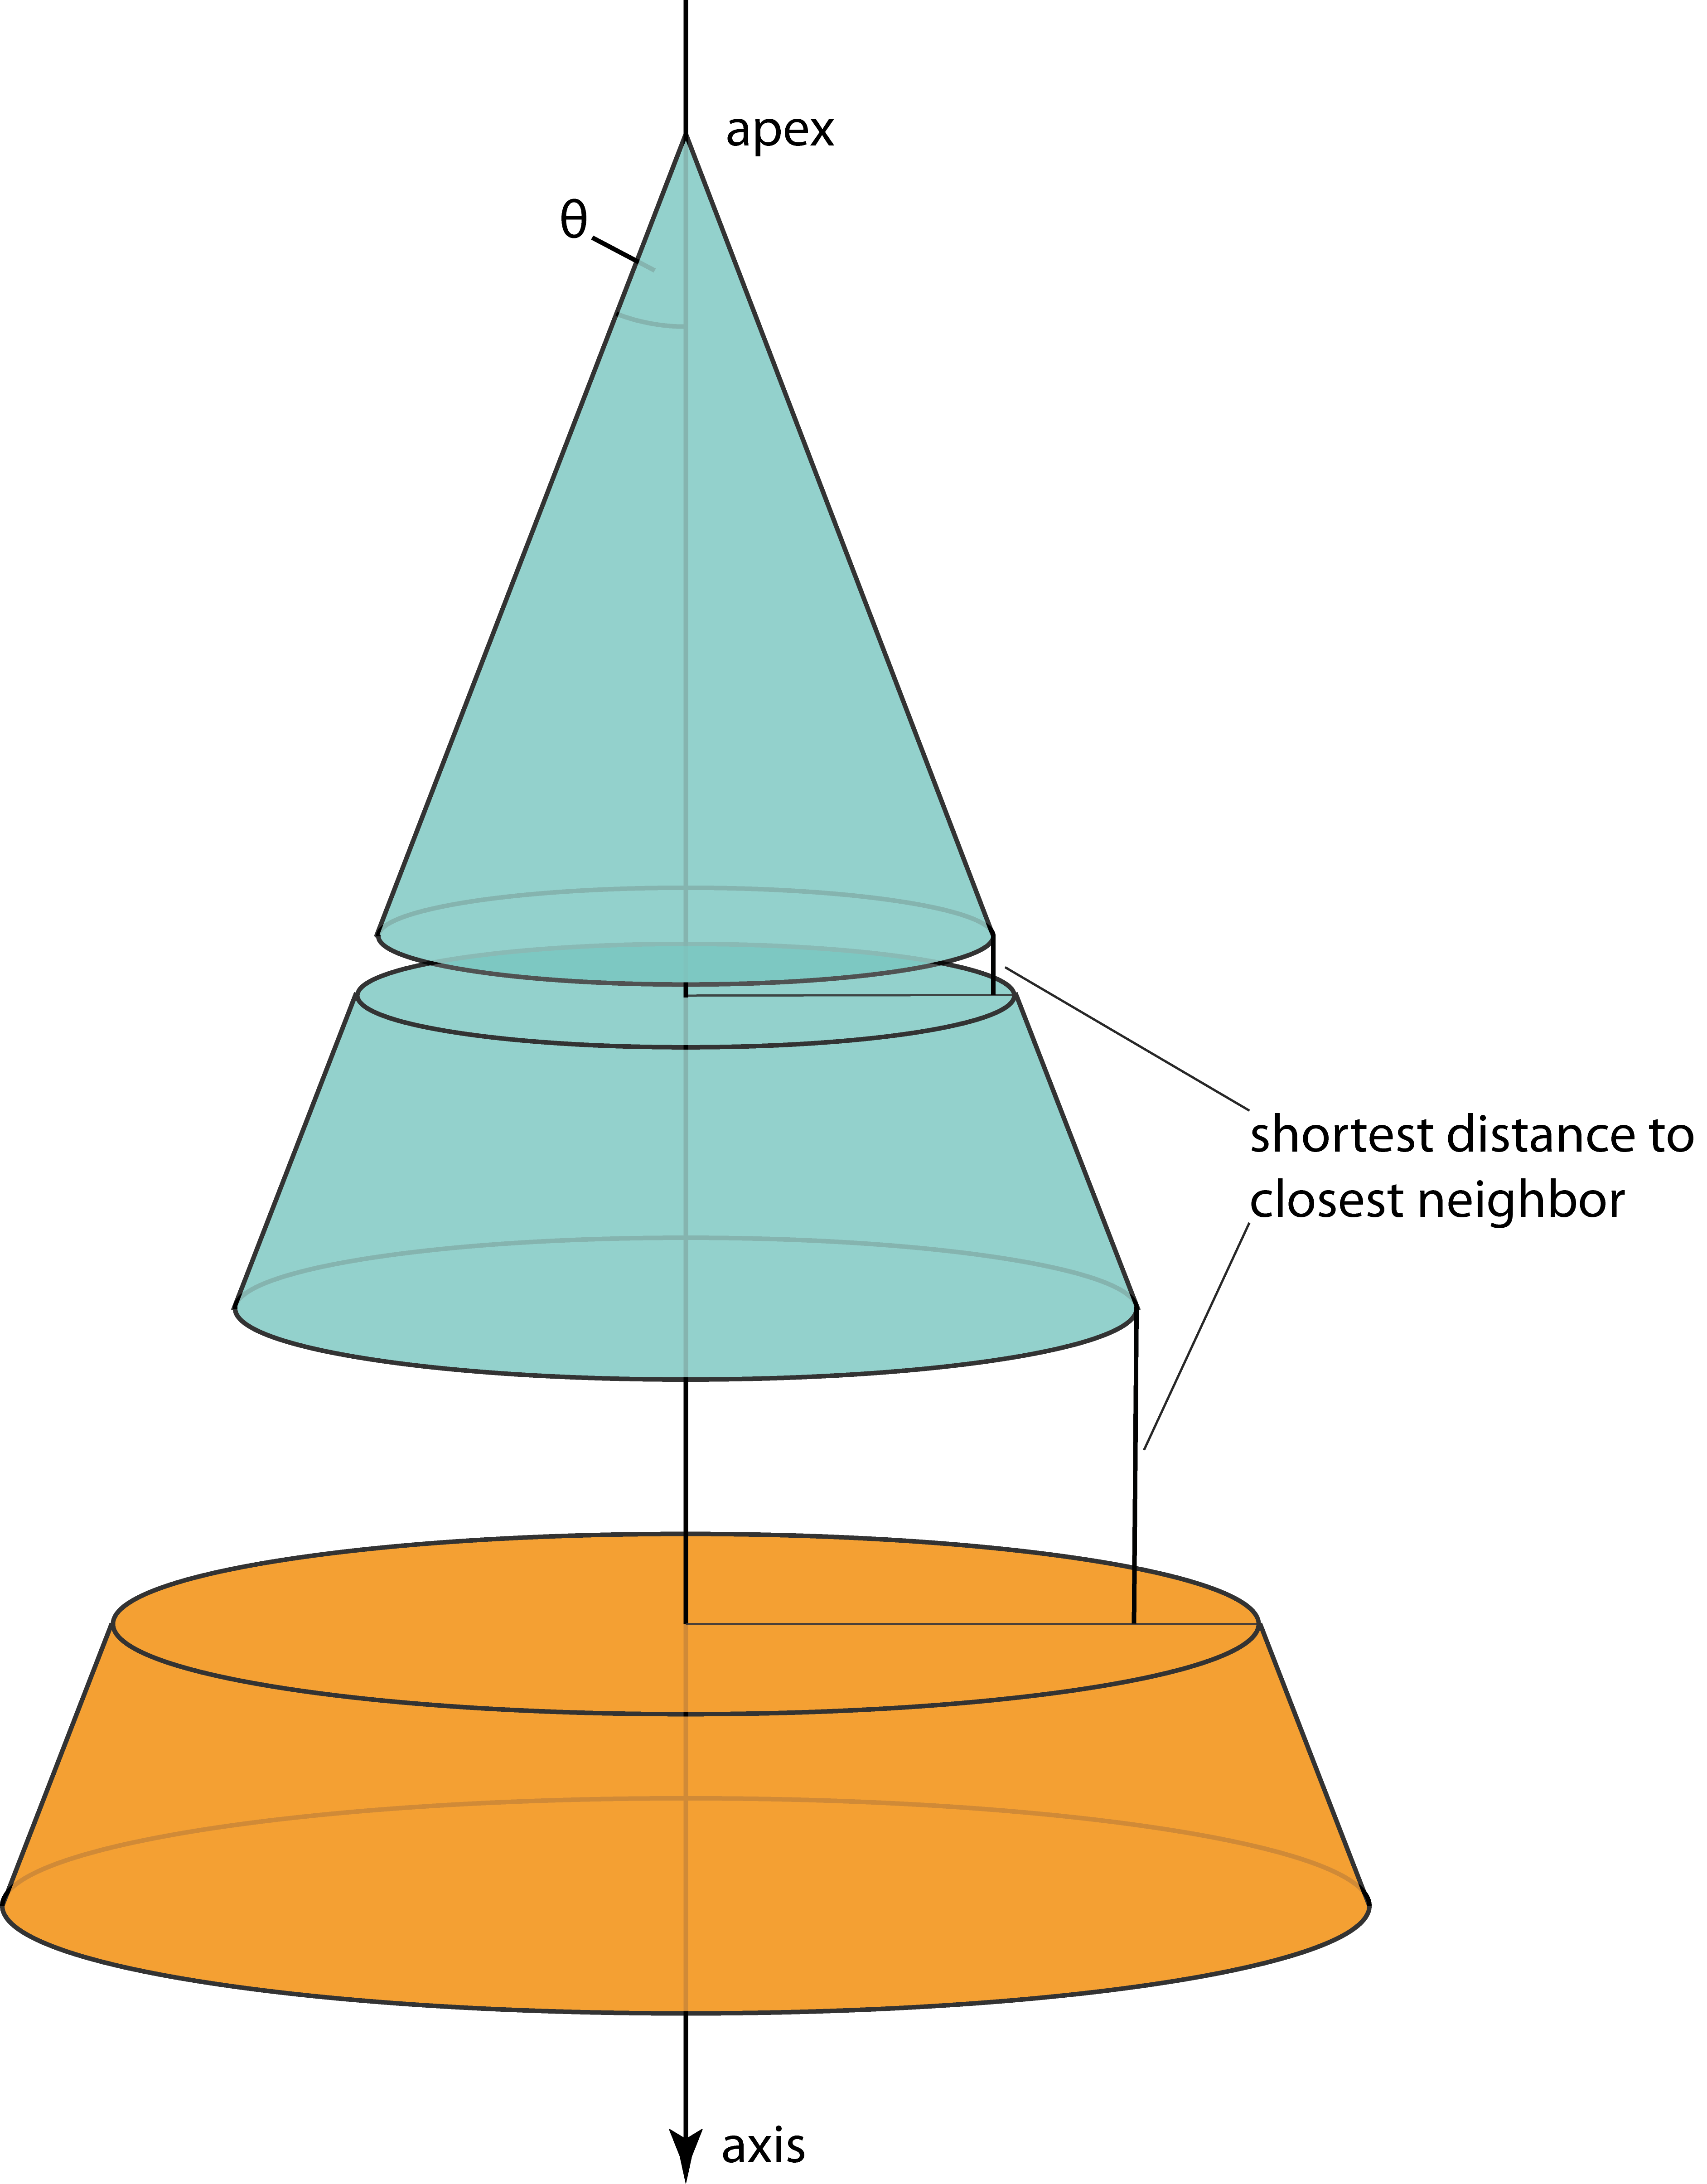
\includegraphics[width=0.5\textwidth]{Shape_Detection/regionGrowingCone.png}%
  }
    \caption{This figure shows a cylinder cluster and a cone cluster build from matching shapes. Shapes that belong to the cluster are colored in turquoise.}
    \label{fig:regionGrowingConeCylinder}
\end{figure}

Figure \ref{fig:regionGrowingConeCylinder} showcases region growing for both, cylinder shapes and cone shapes. The matching heuristic already confirms that the shapes lie on the same axis and share a similar radius. Therefore, instead of a three-dimensional world distance, a one-dimensional distance between two points is sufficient to build a shape cluster. 
\\
\\
The region growing component of the clustering heavily depends on the $\epsilon$ distance threshold. A proper distance threshold that mirrors the region's topology well is the density of an octree node as described in Section \ref{sec:shapeDetectionParameterSelection}. For this task, we chose the density of the node of the base shape, more specific: $\epsilon = density \cdot 2.0$.
\chapter{System Design}
\label{chap:systemDesign}

This chapter discusses the design of the application developed for this thesis. The aim is to develop a stand-alone desktop application to view and interact with out-of-core point clouds. The application offers various methods for the user to interact with the point cloud. The application has three main elements that work together, all controlled by the user. 

\par

Shape detection, as described in Chapter \ref{chap:shapeDetection}, is performed on a sub-region of the point cloud one at a time. Section \ref{sec:user_guided_sd} describes an interactive heuristic that selects an octree node as a region of interest, using the user's cursor position and camera view as input. Using the user's input effectively changes the task of detecting shapes from an automated approach to a user-controlled interaction.

\par

Most interactions presented in this thesis share similar techniques and naming conventions. Therefore, some terms that are used throughout this chapter are defined in Section \ref{sec:termDefinitions}. 

\par

Section \ref{sec:shapePicking} describes a picking algorithm to select a primitive shape from the screen that can later be used as support shape for assisted user interactions. 

\par

Section \ref{sec:interactions} provides detailed information on the additional user interactions that use a support shape as assistance. \textit{point picking, region selection}, and \textit{local level-of-detail increment} are interactions that benefit from the use of a support shape. 


\section{Term Definitions}
\label{sec:termDefinitions}

The basis of all interactions is the user's cursor on the screen. The \textit{pick ray} is a ray that origins from the cursor’s position in world space and goes in the direction of the camera to the cursor position. 
Each interaction iteratively filters the octree's data such that coarse filtering is carried out before finer adjustments are performed on the dataset before choosing a final candidate. Data that survives the coarse filtering is referred to as \textit{candidate}, e.g., candidate nodes or candidate points. 


\section{User-guided Shape Detection}
\label{sec:user_guided_sd}

The shape-detection algorithm is already described in Chapter \ref{chap:shapeDetection}. As the shape-detection computation usually takes several minutes, the approach in this thesis performs this computation on small chunks of roughly the same size of point-cloud data at a time. The octree already provides the point cloud as pieces of spatially neighboring data, such that each node describes an enclosed subset of the point cloud at a specific level of detail. Using chunks of the same size allows the user to expect results in about the same time for each node. This response time should ideally be a fraction of a second, at best less than $250$ milliseconds. 

The \textit{user-guided shape detection} is updated in the background continuously, relying only on the user's current mouse position and view. Thus, only nodes are considered that intersect the pick ray. To be selected as candidate node from the octree, a node must fulfill the following constraints: 

\begin{enumerate}
    \item The node must currently be rendered and visible to the user. 
    \item The node must intersect the pick ray.
    \item The node must contain at least $n$ points, the same amount used as minimal support point count for shape detection.
    \item The node must not have been processed before. Hence, it already contains detected shapes. 
\end{enumerate}

These constraints have the following motivation: Since the user controls the shape-detection process, it makes sense that the user only interacts with what is presented on screen. Therefore, the node must currently be rendered and visible. To reduce the amount of redundant computation, only nodes that contain enough points to fit at least one shape are considered to be candidates. Lastly, the shape-detection algorithm works under the probabilistic assumption that, once it terminates, all shapes in this region are detected. Therefore, nodes that already contain detected shapes do not qualify as candidates as well. 

\par

The culling operation on the octree, described in Section \ref{sec:octree_culling}, returns an octree that only contains nodes that are rendered. Thus, all nodes in this tree are already visible to the user and fulfill constraint 1. Only a single raycast with the pick ray needs to be performed on the culled octree to obtain the set of candidate nodes that fulfill constraints 1 and 2. 

\par

From this set, nodes are eliminated that do not fulfill constraints 3 and 4. The heuristic favors nodes with higher level-of-detail, such that the user receives geometric information for the most detailed parts of the currently explored region first. The projected distance to the nearplane is used to select between nodes with the same level of detail. The node closest to the camera is chosen. 

\par

The selection of a suitable candidate node depends heavily on the camera position. When zooming out, the camera moves away from the scene, thus reducing the render horizon and therefore reducing the maximum level-of-detail. If the node with the highest level of detail is processed already the heuristic chooses a node from a lower level of detail. Thus, a multi-scale representation of the local geometry is constructed over time, creating a level of detail for primitive shapes as well. 


\section{Shape Picking}
\label{sec:shapePicking}

This thesis presents several interactions that are supported by using detected shapes to ease interactions with point clouds. The use of a support shape raises the need for an initial interaction to pick a primitive shape. A raycast is performed on the culled octree using the pick ray to create an initial filtering of octree nodes. From this set of nodes, only those shapes are collected that intersect the pick ray. The picking heuristic prefers primitive shapes of higher level of detail that are closer to the camera. All primitive shapes are collected from the candidate nodes and sorted using a custom key. Primitive shapes that intersect the pick ray come with information on the nearest intersection point and the level of detail. For each intersection point, the $depth$ in the range of $[0,1]$, where $0$ is at the near plane, and $1$ is at the far plane, is calculated. For shapes that intersect the pick ray more than once, the intersection point closest to the camera is chosen. The sort key is composed as follows: 

$$key = level + 1 - depth.$$

The primitive shape with the highest key is chosen as support shape. The composition of the key ensures that a shape with the highest level of detail that is closest to the camera is picked. 

\par

As a primitive shape only covers a small region, limited by the extents of the octree node, and user interactions are usually performed on larger areas, a single primitive shape is not sufficient to provide semantic information to the user. Therefore, once a shape is picked, a cluster is created from this shape using primitive shapes that are similar to this shape. This clustering is described in Section \ref{sec:shapeClustering} in depth. All shapes that match the base shape are collected from nodes that are visible and have the proper level of detail. From this set of shape a coherent cluster is created, such that each shape has a neighbor within $\epsilon$ distance, as described in Chapter \ref{chap:shapeDetection}. A cluster can be seen as a single, multi-level shape and is referred to as \textit{support shape}.


\section{Shape-Assisted Interactions}
\label{sec:interactions}

Creating new interactions is a key topic in this thesis. In 3D applications, classic two-dimensional interaction metaphors, such as \textit{lasso selection} and \textit{point picking}, are limited by the lack of information on the desired depth. In a 3D setting,  these interactions must either guess the desired depth boundaries or ignore them. Furthermore, these interactions lack the possibility to mask out unwanted points from a selection. Unwanted points are selected on a regular basis. Hence, many view changes are necessary to select only points that are of interest. By using a primitive shape as support, the user can easily interact with the point cloud in a way that only points are considered that belong the support shape. 

\par

Figure \ref{fig:interaction_workflow} shows the basic workflow for shape-assisted user interaction. The workflow comprises two major steps. The first interaction is to pick a primitive shape and build a larger cluster from it. This cluster acts as a support shape for the following user interaction. For this interaction, when initialized, all affected nodes are collected, and their point sets are reduced to only those points that are approximated by this shape. A point is filtered if it fulfills the same $\epsilon$-distance and normal-deviation criteria with regard to the support shape as used for the shape detection in Chapter \ref{chap:shapeDetection}. After the filtering step, the actual interaction is performed on the remaining points. 

\par

Sections \ref{sec:pointPicking} and \ref{sec:regionSelection} describe the pros and cons of current state-of-the-art two-dimensional interactions and propose improvements using the workflow mentioned earlier. Furthermore, Section \ref{sec:lod_increment} proposes a technique to locally increment the visible level of detail along structures of interest to amplify details. 


\begin{figure}
    \centering
    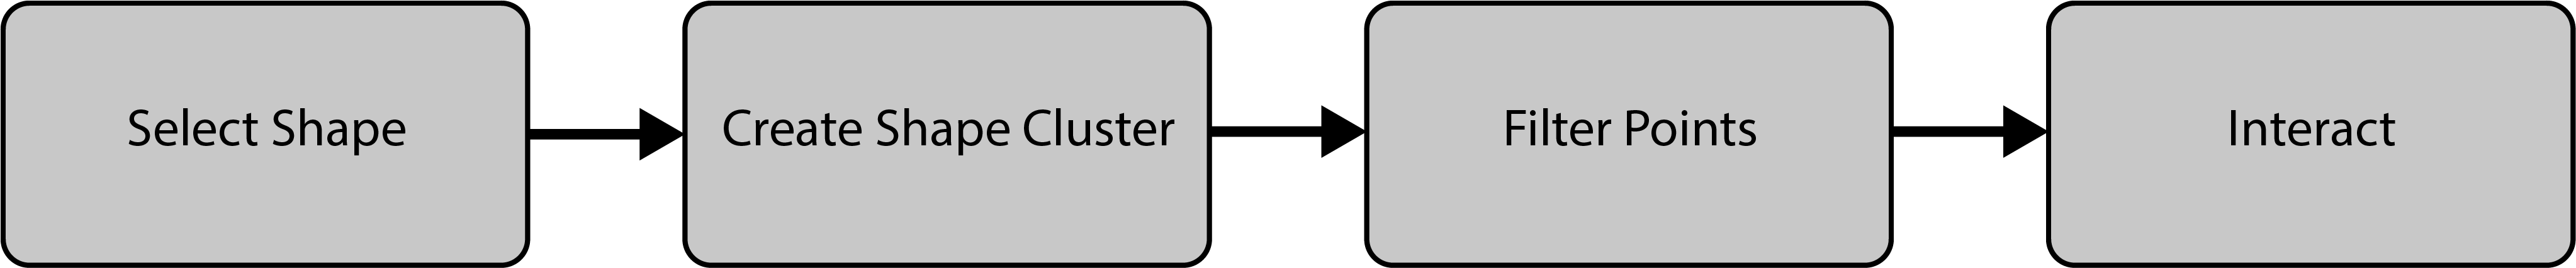
\includegraphics[width=0.8\textwidth]{System_Design/interaction_workflow.png}%7
    \caption[Workflow of an assisted user interaction]
    {The workflow for shape-assisted interactions is divided into two major steps. First, the user picks a primitive shape, from which a larger cluster is created and used as support shape for the following interaction. Upon starting an assisted interaction, the system finds all nodes that are affected by the interaction, reduces the set of points to those that are approximated by this shape and, finally, the interaction (e.g., selection, picking) is performed. }
        \label{fig:interaction_workflow}
\end{figure}
    

    
\subsection{Point Picking}
\label{sec:pointPicking}

\textit{Point picking} describes an interaction where the user is interested in selecting a single point from the scene at a time. The pick radius $r$ denotes the maximum distance of a point to the pick ray for the point to be considered a candidate point. Multiple picking techniques influence the pick radius $r$ differently. The pick radius $r$ can either be constant in world space, constant in screen space or is depended on the depth value. This section gives two examples on how different pick radii influence the consistency of the picking interaction. After that, shape-assisted point picking is discussed.


\subsubsection{Point picking in world space}

The first explored technique is to use a fixed pick radius in world space. The picked point is the point closest to the pick ray in world space. Since the user only interacts with points that are projected onto the near plane, the projection of the pick radius is smaller for points that lie in the background. Therefore, the distance in pixels from the mouse position to the picked point in the background is smaller than the distance to a picked point in the foreground. While this encourages the picking of points in the front, the non-uniform pixel distance introduces inconsistencies as the cursor reacts stronger to points in the foreground. 

\par

Using a simple raycast is not sufficient to find all octree nodes that are affected by this interaction. If the pick ray does not intersect the node's bounding box, it is still possible that the cylinder created by the pick ray and the radius intersects the octree node. Hence, a cylindrical cast must be performed to collect all candidate nodes. 


\subsubsection{Point picking in screen space}

A more consistent way of picking a point is to only use the screen-space information for each point. The mouse position $p$ in screen space combined with the pick radius $r$ create the pick circle $c$. This circle corresponds to the projection of a cone in world space with its apex at the camera position, the pick ray as direction and the opening angle defined by the pick radius. All points that intersect this cone are treated as candidate points. To calculate this intersection, all points are projected to the screen space. The cone intersects a point if $c$ contains the projected point. Then the point with the projection closest to the mouse position is picked. This technique works consistently for different depth values. However, since all points are treated equally, the method does not distinguish between foreground and background points, thus introducing possible depth ambiguities. 

\par

The projection of points can be executed on the GPU by rendering the projected points, paired with an identifier, to a texture. From this texture, a window around the mouse cursor is downloaded, and the closest point is determined. Reading pixels from a texture forces the CPU and GPU to sync and stalls the graphics pipeline. 

\par

Much like picking in world space, the complete set of candidate nodes cannot be retrieved by a simple raycast, as this means that some nodes are node considered that are would intersect the pick cone. Instead, a cone cast is performed to retrieve all affected octree nodes. This conecast is realized by projecting the corners of the node's bounding box onto the near plane and calculating the convex hull polygon. The intersection is determined by the intersection of the polygon with the pick circle in screen space. 


\subsubsection{Shape-Assisted Point Picking}
\label {sec:picking_assisted}

Classic point picking using one of the two described techniques comes with the disadvantage that some constellations of points can influence the picking interaction negatively. The user is forced to change the view to pick an otherwise occluded point from the structure of interest. In some cases, a point in the background is favored over the desired point on a structure in the foreground. \textit{Shape-assisted point picking} utilizes primitive shapes to perform the picking routine only on points that are part of a structure. The user selects a cluster of shapes, thus reducing the number of possible candidate points to only those that belong to this support shape. 

\par

Rather than using a cone or raycast to collect all candidate nodes, only nodes whose bounding boxes intersect the support shape are considered. Furthermore, only points are considered that are approximated by the support shape. This reduction leaves only a handful of nodes and points that follow the curvature of the support shape on which the interaction is performed. 

\begin{figure}[p]
    \centering
    \subcaptionbox{ \label{fig:picking_raycast}}{%
        \includegraphics[width=0.6\textwidth]{System_Design/picking_raycast.png}%7
    }\par\medskip
    \subcaptionbox{ \label{fig:picking_conecast}}{%
        \includegraphics[width=0.6\textwidth]{System_Design/picking_conecast.png}%
    }\par\medskip        
    \subcaptionbox{ \label{fig:picking_assisted}}{%
        \includegraphics[width=0.6\textwidth]{System_Design/picking_assisted.png}%
    }
    \caption
    [Illustration on different picking methods. (a) shows a simple raycast, (b) a cone cast, (c) shows the use of a support shape combined with a sphere cast]
    {Two-dimensional illustration of various picking methods. Candidate points are colored in green; other points are colored in red. The areas in red describe the different volumes in which candidate points are located. (a) showcases a picking process using a simple raycast. The ray combined with a radius constructs a cylinder in world space that contains all candidate points, (b) uses a cone instead. (c) utilizes a selected shape (dark blue) to filter candidate points that are approximated by the shape. A sphere cast is then performed on the filtered points using the unprojected pick radius to obtain the final set of candidate points. }
    \label{fig:picking_overview}
\end{figure}

Due to shapes possibly having front and back sides, such as cylinders and spheres, points on the back of a shape are projected near the mouse position as well. By using the projected distances, points that lie on the back side of the shape might get favored over points that are on the front side of the shape (facing the user). Therefore, point picking is performed in world space using a pick sphere. The sphere's position is the intersection point of the pick ray with the support shape. The sphere's radius is calculated by unprojecting the pick radius to the intersection point. Only points are considered that lie in the pick sphere, constructed by the intersection point and the pick radius. The point closest to the intersection point is then selected. 

\par

This technique not only improves interaction; computation time is reduced as well. Usually, a shape cluster intersects fewer nodes than a raycast result as the cluster's extension is limited to a moderate region in the point cloud. The number of points per node is reduced as well, and distance measures are computed only for candidate points. 

\par

Figure \ref{fig:picking_overview} shows the different picking methods, described in Section \ref{sec:pointPicking}. Figure \ref{fig:picking_raycast} showcases a simple raycast with a radius. The combination of a ray and a radius yields a cylinder, which contains all candidate points on world space. The pick distance is consistent in world space. Figure \ref{fig:picking_conecast} uses a conecast instead. The opening angle is defined by the pick radius in screen space. The pick distance in world space increases the higher the depth value. All points inside the volume are treated equally, introducing consistency in screen space. Figure \ref{fig:picking_assisted} showcases the use of a support shape to filter candidate points. All points that belong to the support shape are filtered before being used as input for a spherecast. 

\begin{figure}
    \centering
    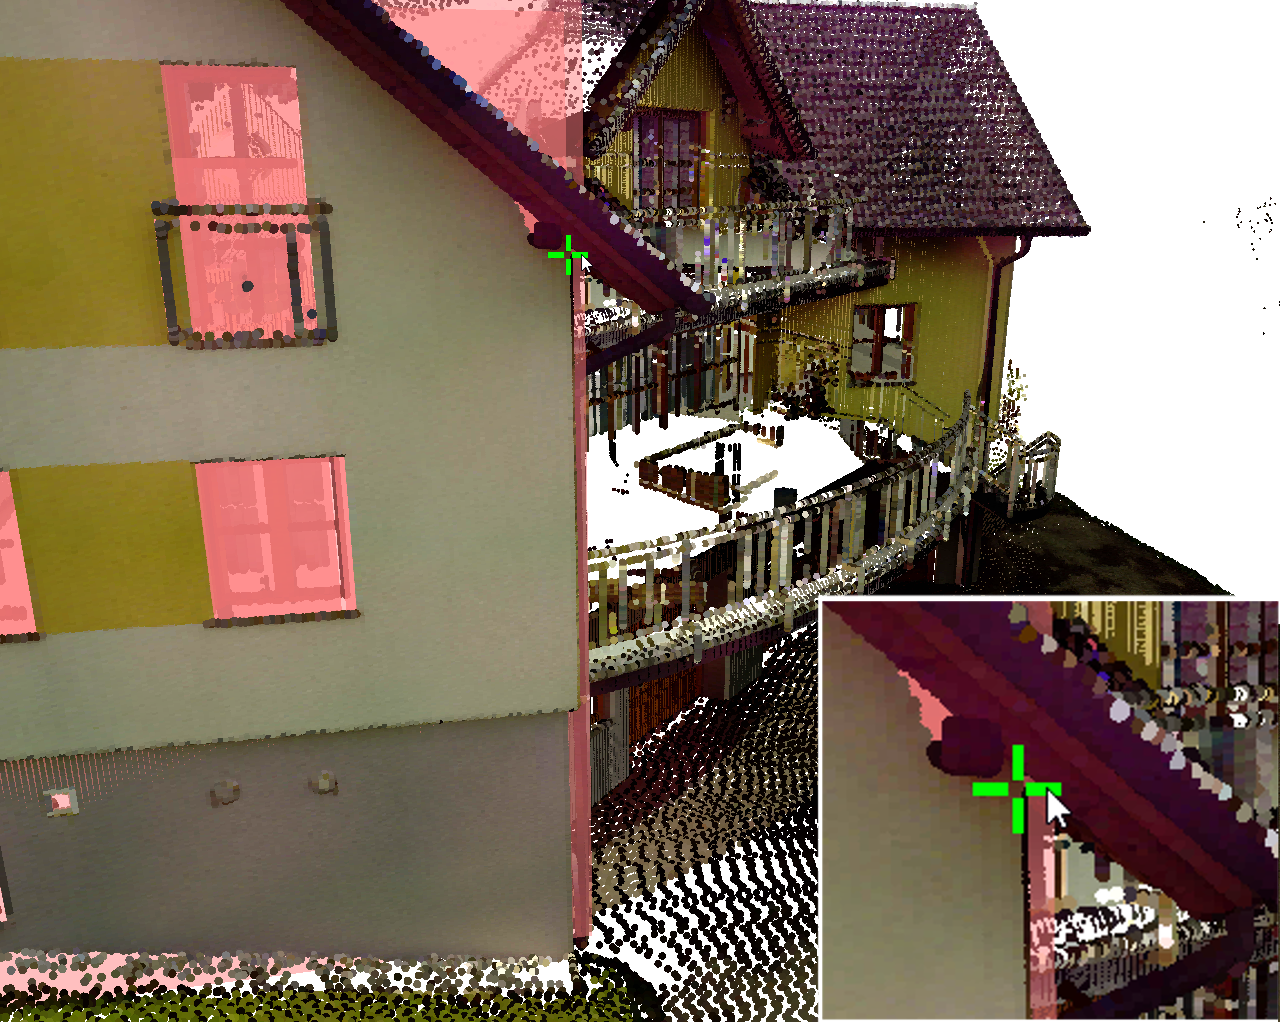
\includegraphics[width=0.8\textwidth]{System_Design/picking_assisted_screenshot.png}%7
    \caption[Screenshot of Shape-assisted Point Picking]
    {Shape-assisted point picking is performed on a shape cluster that represents the wall in the foreground. The cross hair indicates the picked point. Note that the cross hair does not jump to a point in the background even though they would be closer to the cursor in screen space. }
    \label{fig:picking_assisted_screenshot}
\end{figure}

An example of shape-assisted point picking can be seen in Figure \ref{fig:picking_assisted_screenshot}. The cross hair, even though other points' projections are closer to the cursor, sticks to the structure. Picking points on edges is improved in particular since the picking result follows the edge rather than jumping to a point in the background. 


\subsection{Region Selection}
\label{sec:regionSelection}

Region selection aims at selecting a set of points that share certain criteria.
The design for the \textit{shape-assisted region selection} is guided by one seemingly simple example task: \textit{Select points that belong to this wall only}. A wall can intersect with other building elements such as roof, balconies or the ground. In regions close to intersections, it is tedious and cumbersome to only select points on the desired structure. Using two-dimensional interaction metaphors, selecting multiple spatially neighboring points along the same curvature is particularly challenging due to the system not knowing the desired depth boundaries for the selection region. In this section, the benefits of using support shapes for two- and three-dimensional interaction metaphors to select regions of points,  are discussed. 


\subsubsection{Lasso Selection}

The \textit{lasso selection} is a common two-dimensional interaction metaphor used for multiple geometry-based applications. While it is a useful technique to select regions in 2D, drawbacks appear when porting the interaction to 3D. The user draws a polygon onto the screen. All points whose projection lie inside this polygon are selected. Much like point picking, points are projected onto the near plane, the intersection between the point and the lasso polygon in screen space determines whether or not a point is selected. The lasso polygon in combination with the camera view creates a three-dimensional volume, whose area contains all points whose projection lie inside the lasso polygon. Figure \ref{fig:lasso_sketch} showcases the volume created by a lasso polygon drawn onto the screen.

Note that this interaction is computed asynchronously and the selection is performed on the entire octree. Therefore, it is essential that octree nodes whose level-of-detail are too high and are therefore not rendered are still included in this interaction as well. 


\begin{figure}
    \centering
    \includegraphics[width=0.8\textwidth]{System_Design/lasso_sketch.png}%7
    \caption[Illustration of the creation of a lasso selection]
    {The user draws a polygon (red) on the screen (light blue). The constructed three-dimensional area (yellow) contains all points whose projection lie inside the lasso polygon. }
    \label{fig:lasso_sketch}
\end{figure}


\begin{figure}
    \centering
    \subcaptionbox{ \label{fig:lasso1}}{%
        \includegraphics[width=0.5\textwidth]{System_Design/lasso1.png}%7
    }\par\medskip
    \subcaptionbox{ \label{fig:lasso2}}{%
        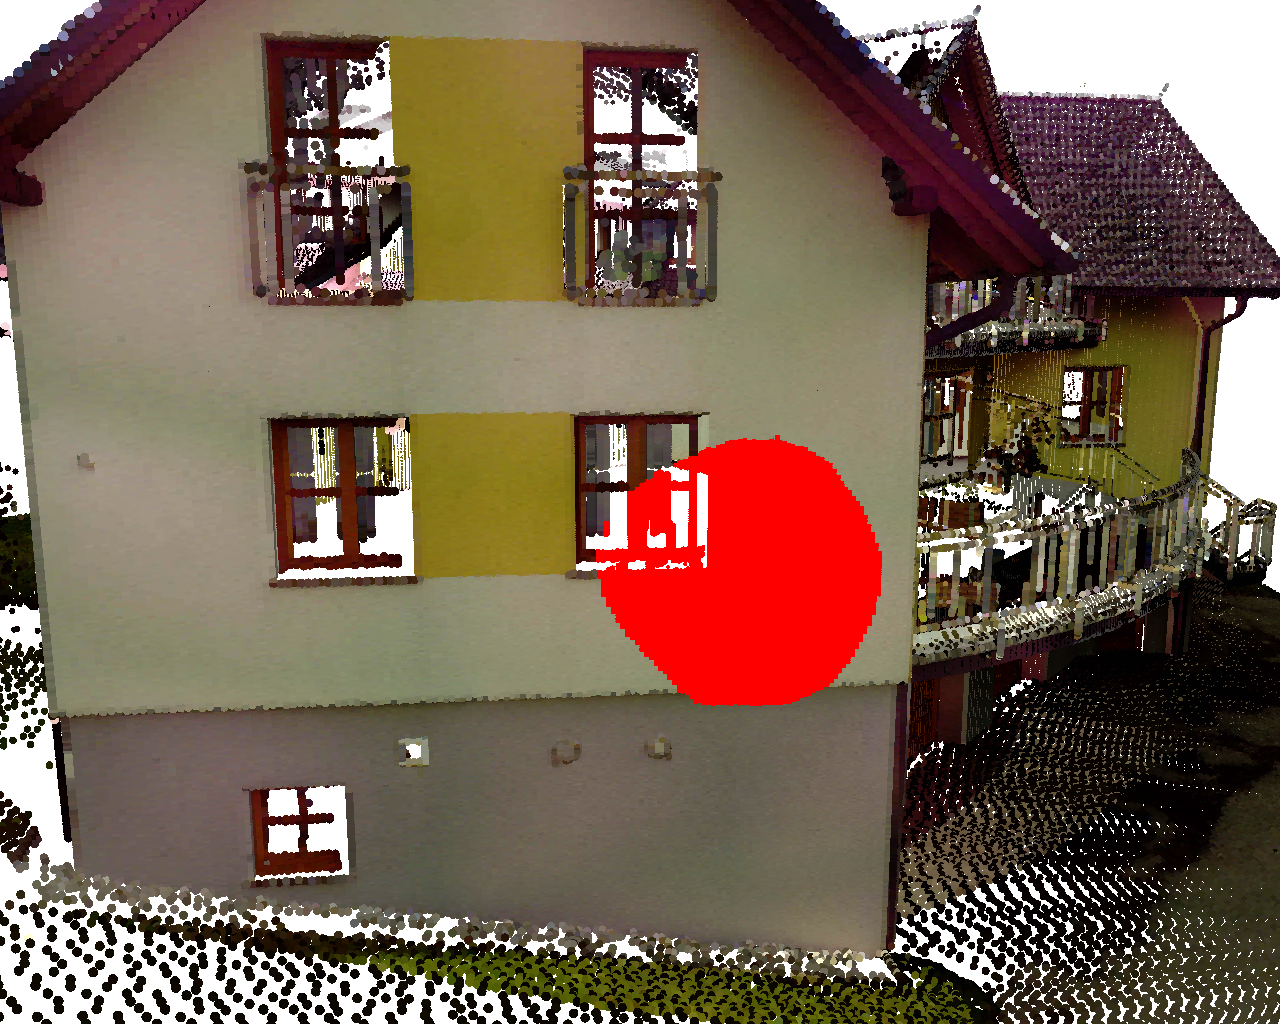
\includegraphics[width=0.5\textwidth]{System_Design/lasso2.png}%
    }\par\medskip        
    \subcaptionbox{ \label{fig:lasso3}}{%
        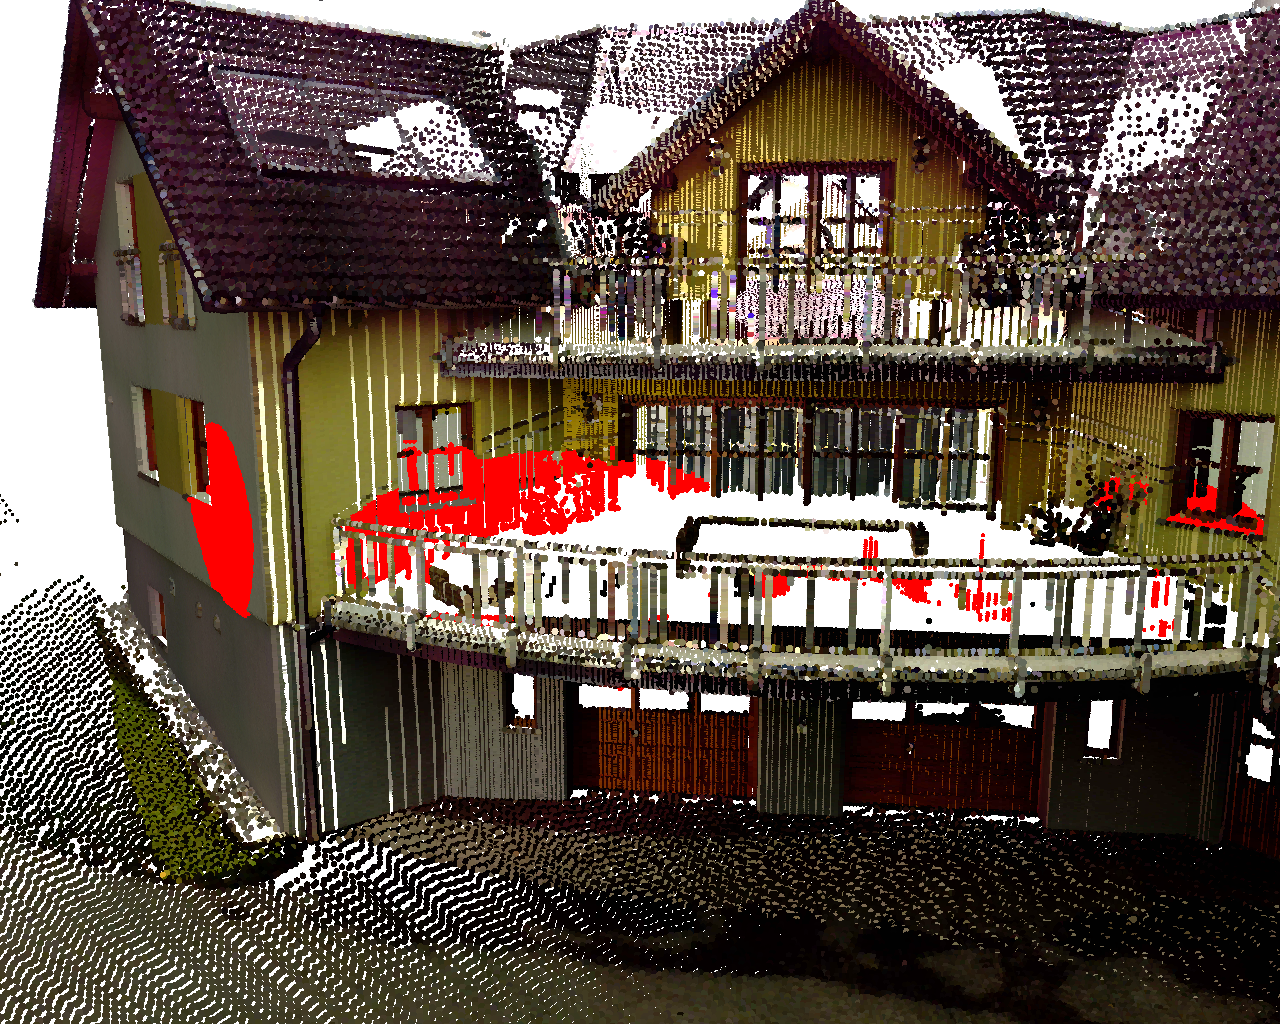
\includegraphics[width=0.5\textwidth]{System_Design/lasso3.png}%
    }
    \caption[Screenshots of the workflow of a lasso selection. (a) shows the lasso, (b) the selected points, (c) shows the selected points from a different angle. ]
    {(a) - (c) show a lasso selection performed on a point cloud. In (a) the user draws a polygon onto the screen. In (b) the selected points are visualized in red. Figure (c) showcases the selection from a different angle. All points that are projected to the area of the polygon are selected. The unintentional selection of points that are obscured by objects in the foreground is a byproduct of the lasso selection. }
    \label{fig:lasso}
\end{figure}


Figure \ref{fig:lasso} shows a classic lasso selection without the use of a support shape performed on a point cloud. The user draws a polygon on the screen. The selected points are highlighted in red. When changing the view, selected points appear that were occluded while drawing the lasso. The user must control the selection distance by hand to minimize this effect. However, to solve the task of only selecting points on the wall, further lasso selections must be applied to remove points from the selection that were selected unintentionally. 


\subsubsection{Shape-Assisted Lasso Selection}

This interaction aims to provide smaller sets of points on which a lasso selection is performed. To construct this smaller sets, the octree is consulted for nodes that intersect the support shape. The number of candidate points per node is reduced by filtering points that are approximated by the support shape. On this reduced set, a normal lasso selection is performed. The result of this interaction is a selection that mimics a lasso selection, with the benefit of not selecting `through` the point cloud. The depth ambiguities of the lasso selection are circumvented by introducing continuous depth boundaries defined by the local curvature of the shape cluster. 

Figure \ref{fig:lasso_assisted} shows the workflow for selecting points on a shape. The shape is selected beforehand by the user. A lasso is drawn on the screen that selects all points that lie within the lasso and belong to the selected support shape. In Figure \ref{fig:lasso_assisted3}, it can be seen that contrary to Figure \ref{fig:lasso3}, no points are selected that do not belong to the support shape.

\begin{figure}
    \centering
    \subcaptionbox{ \label{fig:lasso_assisted1}}{%
        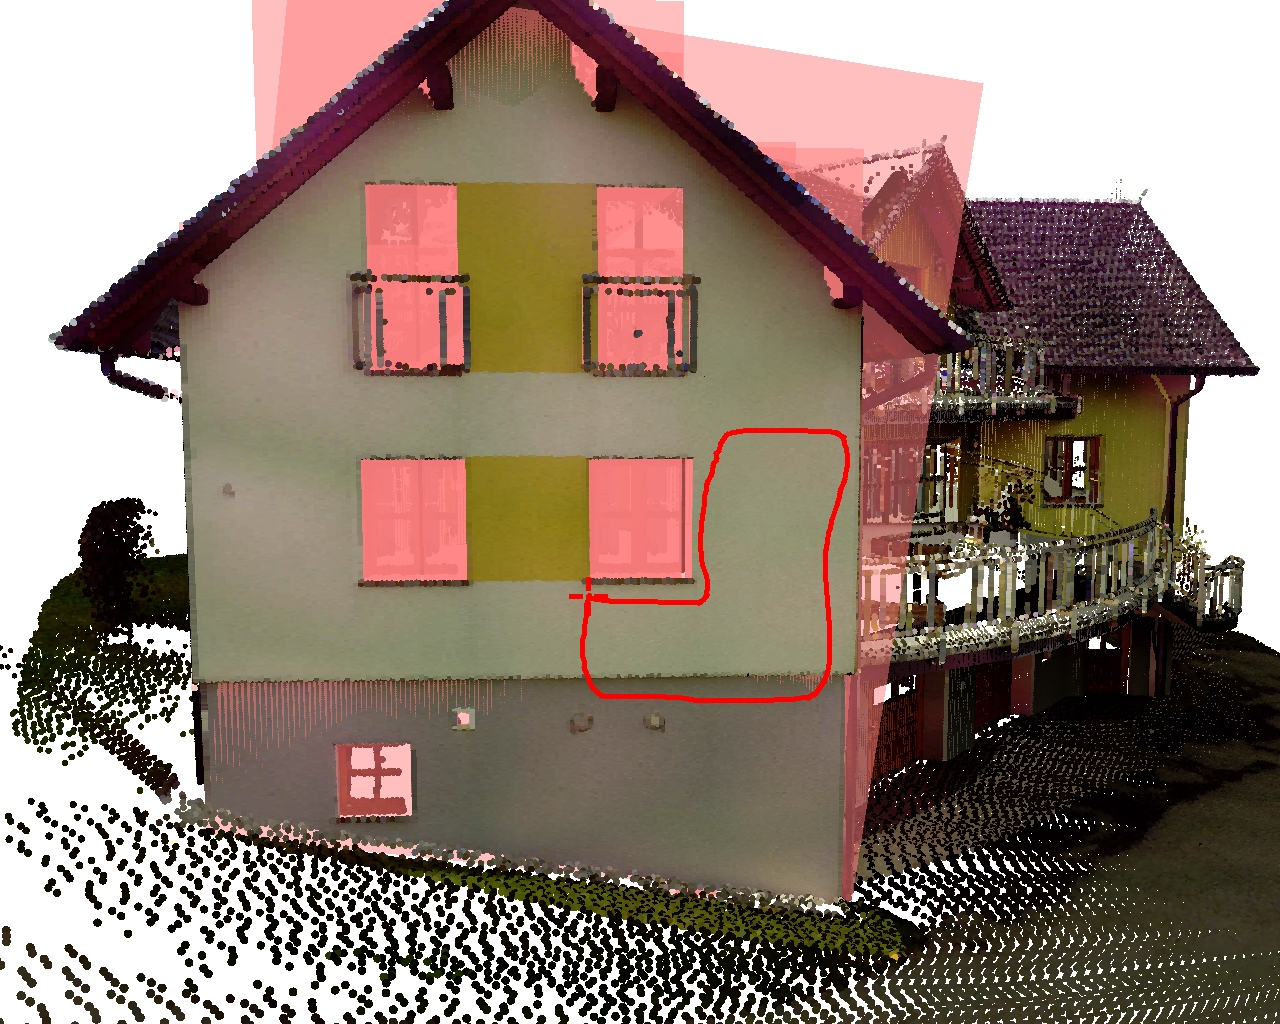
\includegraphics[width=0.5\textwidth]{System_Design/lasso_assisted1.png}%7
    }\par\medskip
    \subcaptionbox{ \label{fig:lasso_assisted2}}{%
        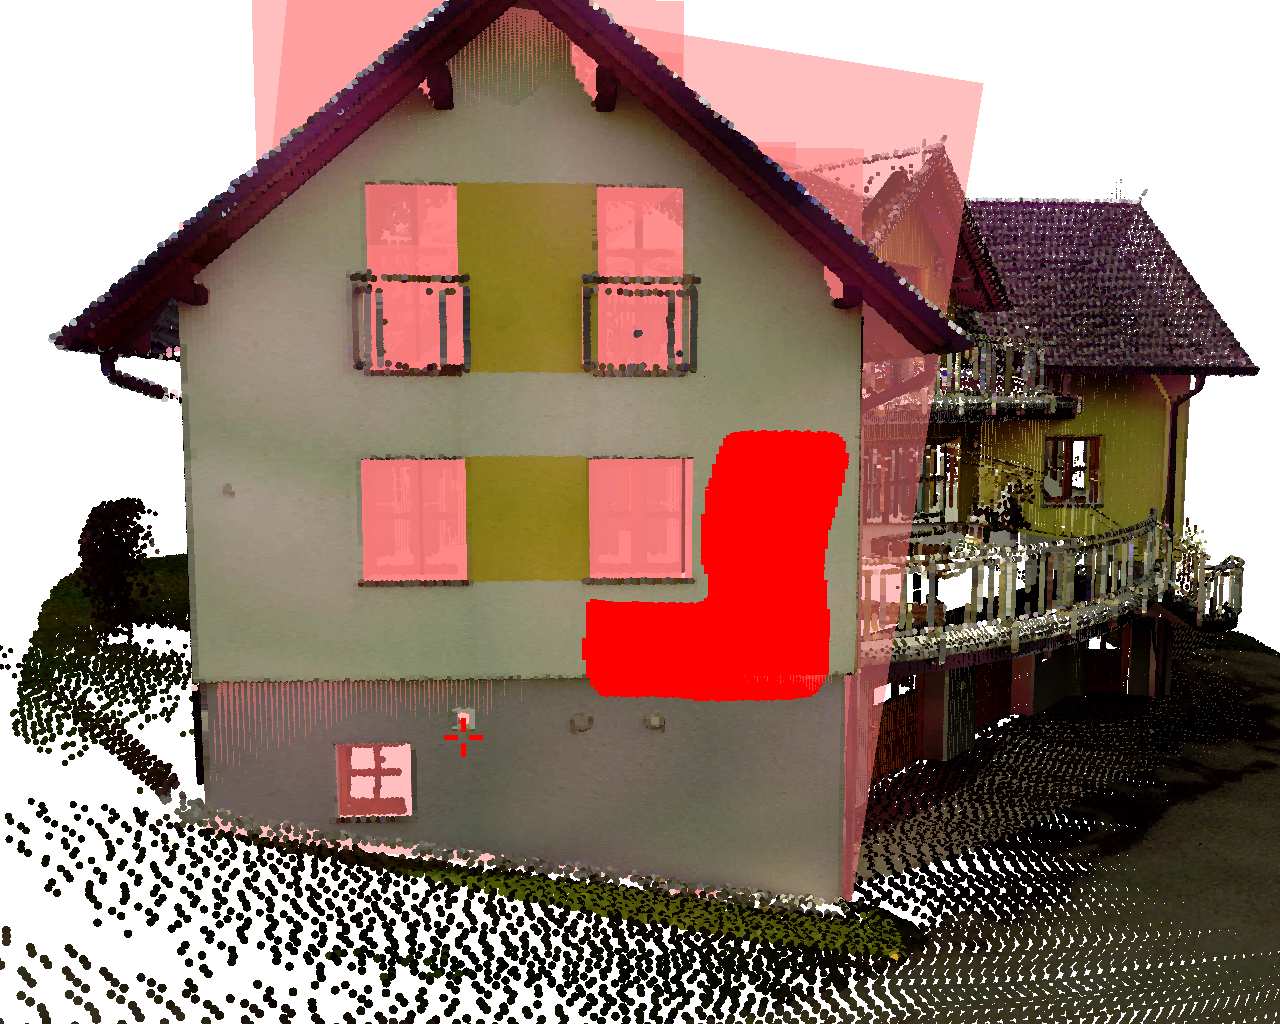
\includegraphics[width=0.5\textwidth]{System_Design/lasso_assisted2.png}%
    }\par\medskip        
    \subcaptionbox{ \label{fig:lasso_assisted3}}{%
        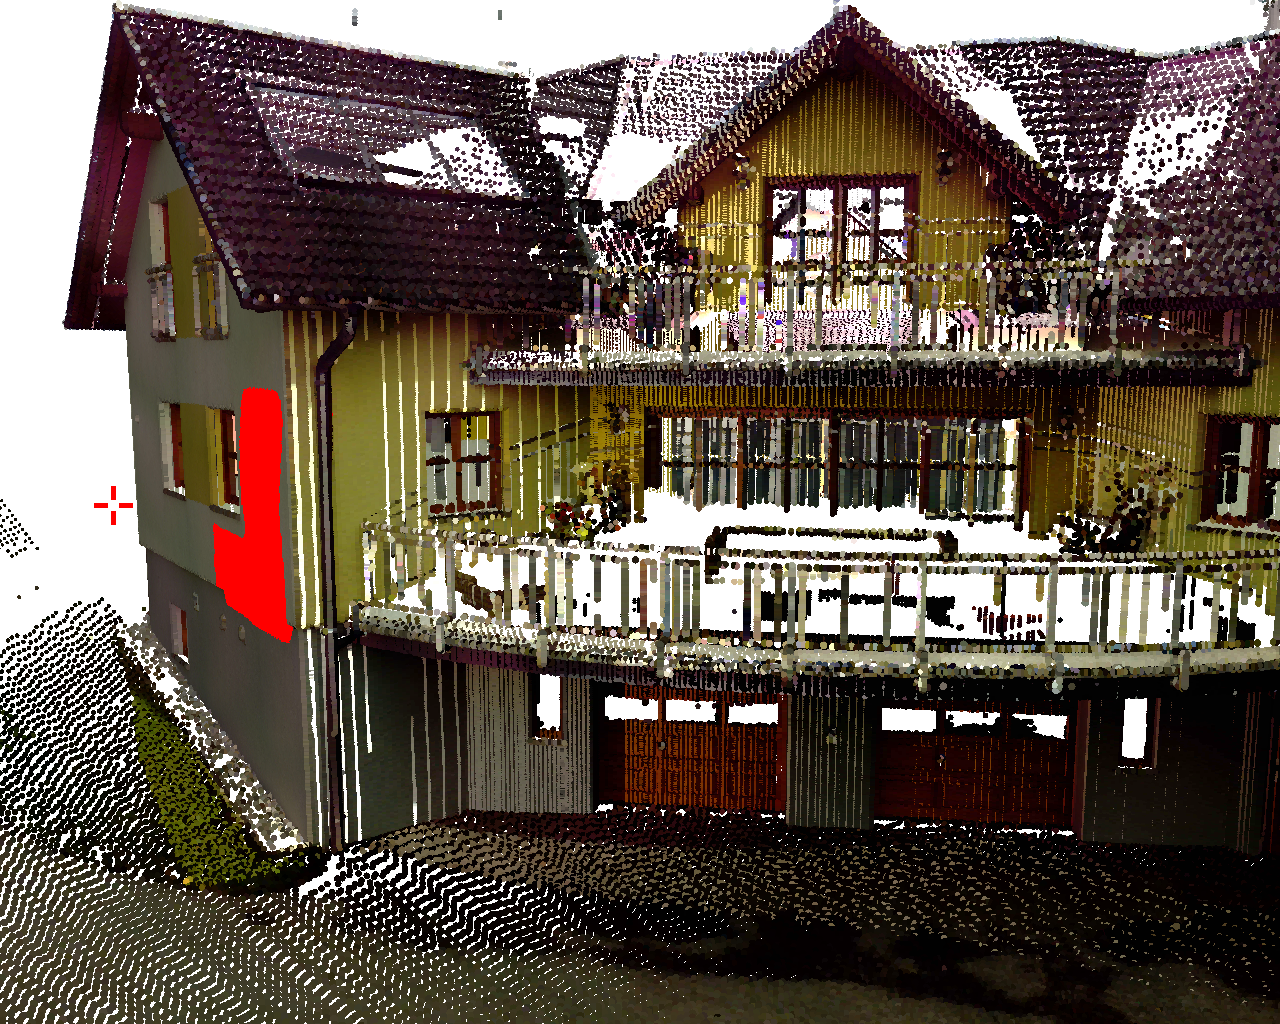
\includegraphics[width=0.5\textwidth]{System_Design/lasso_assisted3.png}%
    }
    \caption[Screenshots of the workflow of a shape-assisted lasso selection. (a) shows the lasso and the support shape, (b) the selected points, (c) shows that only points are selected on the support shape.]
    {(a) - (c) show a shape-assisted lasso selection performed on a point cloud. The front-facing wall is selected as support shape by the user. The shape cluster is visualized in light red. In (a) the user draws a polygon on the screen after selecting a shape as support shape. (b) shows the selected points visualized in red from the same point of view. Upon view change, it can be seen that this interaction only selects points that belong the shape cluster. }
    \label{fig:lasso_assisted}
\end{figure}


\subsubsection{Volumetric Brush}

The \textit{volumetric brush} \cite{weyrich2004post, scheiblauer2011out} is designed in such a way that a volume is projected onto the foremost geometry. Points that intersect this volume are considered to be selected. To retrieve the projected position of the volume (e.g., a sphere) the depth buffer is consulted, and the depth value for the current mouse position is retrieved. The world position is the unprojection of the mouse position's $xy$-coordinates and the depth value. 

Since this technique follows the foremost geometry only, sudden depth changes occur if different geometry occludes the area of interest. Thus, view changes are still required to achieve the example task. In regions close to intersections with other structures, such as below the roof, the user must control the size of the volume to not select points on neighboring structures. 


\subsubsection{Shape-Assisted Volumetric Brush}

The volumetric brush can easily be adapted to be used in combination with support shapes. Instead of consulting the depth buffer to reconstruct the cursor’s world position, the pick ray is intersected with the selected support shape, thus resulting in a three-dimensional world position. The octree is consulted for nodes that intersect the support shape, and the sets of points are reduced to only those that are approximated by the support shape. 
Figure \ref{fig:brush} shows a \textit{shape-assisted volumetric brush} interaction performed on a wall. The wall creates as a cluster of planes. Only points are selected that belong to this cluster. 

\begin{figure}
    \centering
    \subcaptionbox{ \label{fig:brush_assisted1}}{%
        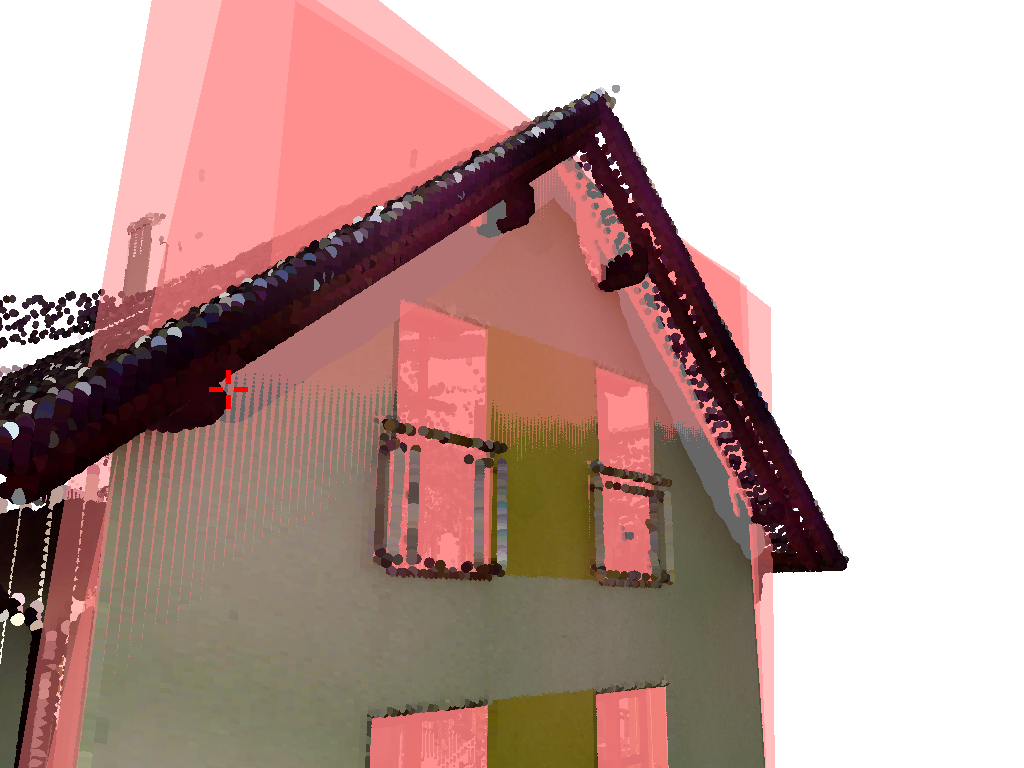
\includegraphics[width=0.8\textwidth]{System_Design/brush1.png}%7
    }\par\medskip
    \subcaptionbox{ \label{fig:brush_assisted2}}{%
        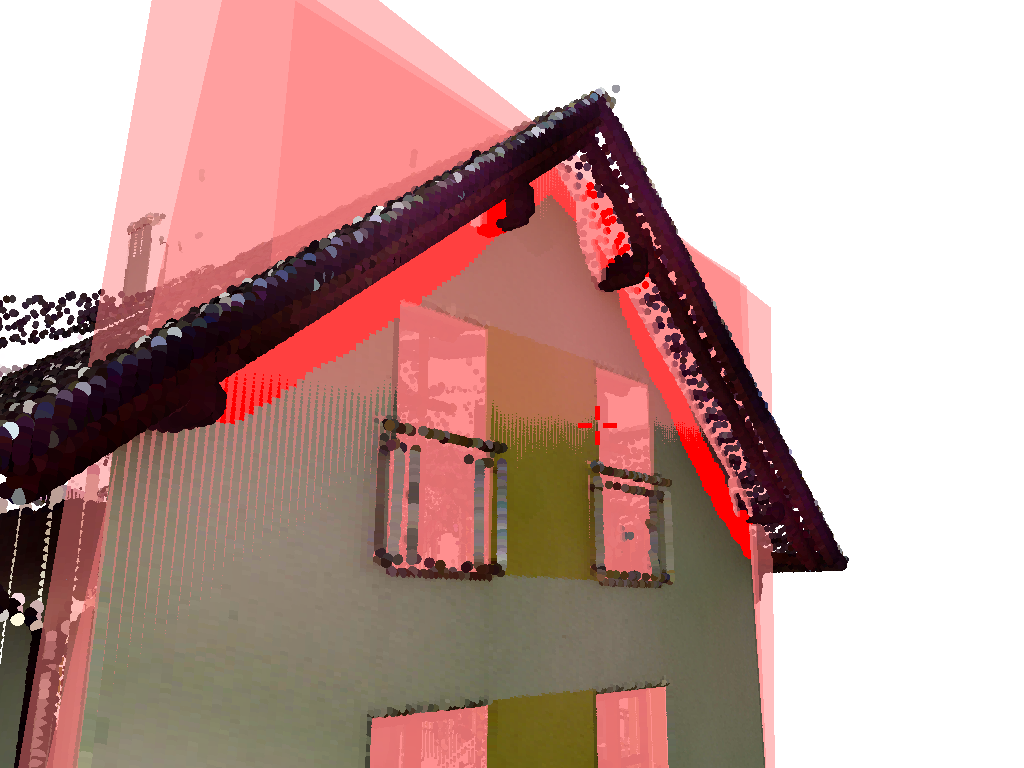
\includegraphics[width=0.8\textwidth]{System_Design/brush2.png}%
    }
    \caption[Workflow of the shape-assisted volumetric brush. (a) shows the trajectory of the brush, (b) shows the selected points. ]
    {This figure shows a shape-assisted volumetric brush selection performed shape cluster (transparent red) detected in a point cloud. In (a) the trajectory of the brush is shown as subsequently rendered spheres(grey). (b) shows the selected points for this brush interaction. Even tough some points of the roof structure are intersecting the brush, they are not selected. }
\label{fig:brush}
\end{figure}


\subsection{Shape-Assisted Local Level-of-Detail Increment}
\label{sec:lod_increment}
    
To further investigate the local structures of a point cloud, the currently rendered maximum level-of-detail might not suffice. The highest level of detail is chosen such that the GPU is not overloaded and the balance between detail and performance is retained. Temporarily adding a handful of additional nodes is sufficient to provide more detailed information, and does not pose an enormous impact on performance. 
    
\par

Section \ref{sec:octree_culling} describes the culling heuristic to create an octree that only contains nodes that are rendered for the current frame. This heuristic uses view-frustum culling paired with a level-of-detail culling decision. However, for the \textit{Shape-assisted local level-of-detail increment} the culled octree is not sufficient, and more detailed point information needs to be fetched from the original octree. 

\par

Each node of the culled octree is compared with its counterpart in the original octree. All children of the counterpart node that were culled by the level-of-detail decision, but not by view-frustum culling, are collected in an initial set. These nodes share the property that each of them could be rendered on the screen, but its level of detail is too high for the current scene. The same property applies to the successors of each node as well. A \textit{level-of-increment} parameter $i > 0$ controls the number of additional levels of detail that should be displayed for this interaction. For $i=1$, e.g. the children, the initial set needs no further processing. Thus, it can be used as candidate set for the next step directly. For a level-of-increment parameter $i>1$, all $(i-1)^{\text{th}}$ successors of the nodes from the initial set are taken as candidate set instead. 

\par

By adding smaller nodes with a higher level of detail, the overall detail in the scene is increased. However, by adding nodes without additional point filtering, noise and unwanted structures are amplified as well. Therefore, this interaction utilizes a shape cluster, selected by the user, to amplify detail only on structures of interest. The candidate set is filtered further, such that only those nodes remain that intersect the support shape. For each node from this final set, only those points that are approximated by the support shape are added to the scene.

    \begin{figure}
        \centering
        \subcaptionbox{ \label{fig:lod_increment1}}{%
            \includegraphics[width=0.8\textwidth]{System_Design/lod_Increase.png}%7
        }\par\medskip
        \subcaptionbox{ \label{fig:lod_increment2}}{%
            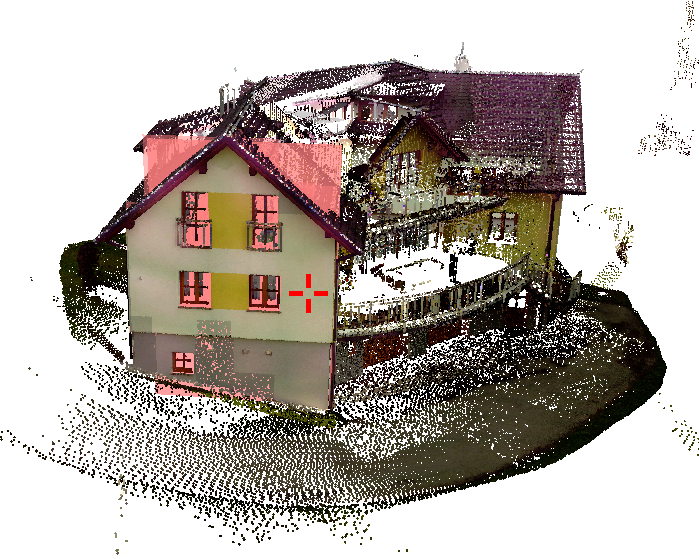
\includegraphics[width=0.8\textwidth]{System_Design/lod_Increase2.png}%
        }
        \caption[Comparison of a scene with and without shape-assisted level-of-detail increment.]
        {This figure shows the benefits of shape-assisted level-of-detail increment for a point cloud. (a) shows the currently rendered structure, as well as as shape cluster that is currently selected (red). (b) shows the scene with amplified details along the structure. The additional points are rendered without lighting to appear brighter.}
        \label{fig:lod_increment}
    \end{figure}
    
Figure \ref{fig:lod_increment} showcases the difference in a scene with and without amplified details along a wall. The selected support shape is rendered in transparent red, while the additional points are rendered without lighting to appear brighter. In the intersecting octree nodes, only those points are rendered that fulfill the shape's score function. 
    
    

\chapter{Implementation}
\label{chap:implementation}

This chapter gives an overview of implementation details for this thesis. The implementation of the application is guided by the \textit{functional-first} programming paradigm. \textit{Functional-first} takes inspiration from functional programming, as well as other paradigms, such as object-oriented programming. However, the majority of the application is written in a purely functional way, with connections to non-functional components, such as .NET libraries for multi threading or Schnabel et al.'s shape detection implementation \cite{schnabel-2007-software}. The backbone of the application is the Aardvark platform \cite{aardvark}. It is a functional-first incremental rendering engine in active development at the VRVis Zentrum für Virtual Reality und Visualisierung \cite{vrvis}.

\par

This chapter starts with an introduction to functional programming and the programming language \verb|F#| \cite{FSharp} before introducing the key features of the Aardvark platform in Section \ref{sec:aardvark}. The primary data structure used for organizing the point cloud data is an octree with out-of-core capability. A set of functions that simplify querying with the octree is proposed in Section \ref{sec:funcOctree}. 

\par

Multiple coroutines are performed in the background and produce a stream of updates on the point-cloud data. The multi-threaded architecture of the application is discussed in Section \ref{sec:multithreading}. Section \ref{sec:rendering} concludes this chapter by briefly discussing implementation details of the point-cloud rendering system. 


\section{Functional Programming}
\label{sec:funprog}

Functional programming is a paradigm that views every expression as a mathematical function. The result of each expression is either an elemental data type or a functional type. A core difference to other programming paradigms is the type-level representation of functions (same as data). Thus, functions can be used as input for other functions and have a distinct type defined by its parameters and result. A simple example of a function in \verb|F#|: 

\begin{lstlisting}[language=FSharp]
let square (i : float) : float = i * i 
\end{lstlisting}

This function is of type \verb|float -> float|. It takes a \verb|float| as input and returns a \verb|float|. This function type can be used as input parameter as well. A definition for a function that takes a function as parameter looks as follows: 

\begin{lstlisting}[language=FSharp]
let compute (i: float)(f : float -> float) : float = f i
\end{lstlisting}
Its type is \verb|float -> (float -> float) -> float| and is used as such: 
\begin{lstlisting}[language=FSharp]
let result = compute 10.0 square
\end{lstlisting}

\verb|result| is an expression that executes the \verb|compute| function with arguments $10.0$ of type \verb|float| and \verb|square| of type \verb|float -> float|. Even though this is just a simple example, it showcases the strength of functional programming.  Using functions as input allows the user to create complex and dynamic computations with ease. 

\par

Each expression in a functional context is mathematically defined, parameter space and result space are fully known and must be fully defined on type level. No values that the program does not expect ever occur, thus eliminating undefined behavior. 
Functional programming tries to limit mutation, e.g., change of an external variable's value (program state), as much as possible. A program without mutation is called \'pure\'. Each call to a pure expression with the same parameters must produce the same results. External mutation can change the behavior of expressions that depend on the mutated field, thus changing the result without changing the input. Therefore, avoiding mutation means avoiding undefined behavior.
Finally, strict purity and full type-level specification make it possible to reason and construct proofs about programs. This gives the programmer tools to manage very high complexity and reduces the need for debugging significantly.

\par

\verb|F#| is a functional programming language developed and maintained by Microsoft \cite{Microsoft}. The language is fully integrated into the .NET framework \cite{DotNet} and is built upon the Common Language Infrastructure \cite{CLI}, thus allowing it to use resources written in other languages, such as C\# \cite{CSharp}. Even though F\# is a functional language, it also supports object-oriented programming, such that classes with member functions can be used as well. 


\section{Aardvark}
\label{sec:aardvark}

The Aardvark platform \cite{aardvark} is an implementation of research results on the field of incremental rendering \cite{worister2013lazy, haaser2015incremental} and semantic shader composition \cite{haaser2014cosmo, haaser2014semantic}. 
The key feature of the Aardvark platform is incremental rendering. In a conventional engine, updates are performed periodically. Each scene object is re-evaluated, even though the simulation or user input may not yield any changes. Incremental rendering counters this overhead by reacting to changes in a way that only components that depend on changed values are re-evaluated. This section describes some of Aardvark's key features that are used throughout this thesis. Section \ref{sec:adaptive} shows the language-specific constructs on how to build adaptive blocks that react to changes. A \textit{scene graph} represents an object hierarchy in the scene. Section \ref{sec:isg} describes the composition of a scene graph using only a handful of lines of code. 

 
\subsection{Adaptive - IMod - transact}
\label{sec:adaptive}

As mentioned in Section \ref{sec:funprog}, mutations are often the cause of undefined behavior and bugs. To introduce state-changeable variables into a functional environment, Aardvark provides the \verb|IMod<'a>| type. This generic type is a wrapper around a particular value, whose value might change over time. The programmer does not care about the concrete value, and only specifies the computation applied to the value instead. Aardvark contains an extensive implementation for a three-dimensional transformation, called \verb|Trafo3d|. The type \verb|IMod<Trafo3d>| listens to changes of the transformation. The following example shows the composition of a model transformation from a position, scale, and rotation, all of which can change over time. 

\begin{lstlisting}[language = FSharp]

let position    : IMod<V3d> = ... 
let scale       : IMod<V3d> = ... 
let rotation    : IMod<V3d> = ...

let trafo : IMod<Trafo3d> = 
    adaptive {
    
        let! sc  = scale
        let! rot = rotation
        let! pos = position
        
        
        let S = Trafo3d.scale sc
        let R = Trafo3d.Rotation rot
        let T = Trafo3d.Translation pos
        
        return S * R * T
    }
\end{lstlisting}

The \verb|adaptive| computation expression builder allows the system to keep track of the state of all IMods that are accessed using the \verb|let!| operator. This \textit{binding} operator makes a computation react to their changes. The result of the adaptive block, again, is an IMod<Trafo3d>. If one of the accessed IMods changes its value, the code below, including the \verb|let!| statement, is reevaluated. The computation is kept minimal using caching. 
\\

To actively change a value, a subtype of \verb|IMod<'a>|, \verb|ModRef<'a>| is needed. The type \verb|ModRef<'a>| contains the functionality to allow changes to the value, thus causing re-evaluation. All state transactions are collected and executed sequentially, thus reducing the number of re-evaluations and circumventing race conditions. Each change must be wrapped in a \verb|transact| function, representing transactional logic. 
The following example uses the Aardvark-specific mouse callback function to trigger a reevaluation based on mouse movement. The Move-callback is called each time the mouse moves and provides the user with the old position and the new position. The difference on the x-axis controls the y-value of the rotation. 

\begin{lstlisting}[language = FSharp]
let mouse : IMouse = ...

let rotation : ModRef<V3d> = Mod.init V3d.OOO

mouse.Move.Values.Add(fun (oldPos : PixelPosition, newPos : PixelPosition) -> 
    let delta = 
            newPos.NormalizedPosition.X - oldPos.NormalizedPosition.X
    let angle = delta * 2.0 * Math.Pi
    
    let newRotation = 
            rotation.GetValue() + V3d(0.0, angle, 0.0)
    
    transact(fun () -> Mod.change rotation newRotation)
    )
\end{lstlisting}

The \verb|ModRef| \verb|rotation| can then be used bound within an \verb|adaptive| block.
\\
Transactions are usually used to handle user input. However, asynchronous computations that produce results in parallel use transactions as well to mitigate race conditions on shared data and notify the rest of the program on completion. 


\subsection{Scene-graph composition}
\label{sec:isg}

A scene graph (\verb|ISg|) contains all information that is needed to render an object. A common paradigm in functional programming is to separate functionality from data, such that the functions that utilize this data are stored in a different namespace than the data. In combination with the pipe operator ($|>$) clean and easy-to-read code can be produced. The following example showcases the composition of an \verb|ISg|. 

\begin{lstlisting}[language = FSharp]

// Transformations
let trafo :  IMod<Trafo3d> = ... 
let view  :  IMod<Trafo3d> = ...
let proj  :  IMod<Trafo3d> = ...

// IndexedGeometry contains triangles to render
let geometry : IndexedGeometry = ...

// The renderpass for this scenegraph
let renderPass : RenderPass = ...
// The shader (surface) to render the geometry with
let shader : IMod<ISurface> = ...
// Create scenegraph
let sg = geometry   |> Sg.ofIndexedGeometry
                    |> Sg.trafo trafo
                    |> Sg.viewTrafo view
                    |> Sg.projTrafo proj
                    |> Sg.pass renderPass
                    |> Sg.surface shader
\end{lstlisting}

The field \verb|sg| represents a scene graph with transformations, geometry, shader and render pass without the need of complicated constructors or setter functions. Furthermore, an own implementation of \verb|ISg| can easily extend the functionality without reimplemented procedures for this particular type. This extensibility is implemented using a dynamic object attribute mechanism.


\subsection{Out-of-core capabilites}

The Aardvark platform contains functionality to handle out-of-core data. The type \verb|Database| provides means to store data. A chunk of data stored in this database is called \verb|thunk<'a>| where \verb|'a| is the type of the data to be stored. The following code shows how to create a \verb|thunk<'a>|. 

\begin{lstlisting}[language = FSharp]
    let db : Database = ...
    let data : 'a     = ...
    
    let stored : thunk<'a> = db.ref data
\end{lstlisting}
When a \verb|thunk| is loaded from the database, its content is not loaded into memory yet. Only when accessing the data directly, it is loaded into memory. This technique is referred to as \textit{lazy evaluation}. The data is held in memory as long as the thunk lives. Therefore it is crucial to keep track of unused thunks and dispose of them regularly, thus freeing memory. 


\section{Functional Out-of-core Octree}
\label{sec:funcOctree}

Chapter \ref{chap:octree} already provides information on the capabilities of the octree. This section describes implementation details of the octree's structure using out-of-core mechanics and custom parametric functions for convenient octree queries. 


\subsection{Structure}

The octree's out-of-core capability is managed by an interleaved structure of \verb|thunks|. Each \verb|OctreeNode| contains an array of points. However, the array is not stored directly; it is stored as a \verb|thunk<Point[]>|. Its children are stored in an array of thunks (\verb|thunk<OctreeNode>[]|). The points are stored as a single \verb|thunk|, the reason for storing the node's children in separate thunks is not to load all children into memory when only a subset of children is accessed. Other information such as the centroid, density, rkd tree, and the detected primitive shapes are stored as \verb|thunks| as well. 


\subsection{Elementary functions}

The interaction methods described in Section \ref{sec:interactions} rely heavily on the efficient collection of octree nodes that fulfill certain criteria. Thus, a set of routines is implemented that can easily be parameterized and reused. \verb|F#| collections contain several functions that use a lambda function as input and perform this function on elements in the collection. Two examples are \verb|map| and \verb|filter|. Both take two arguments, an array and a function that takes an element as input. All operations on collections can be composed from these basic functions. This is called the \textit{mapReduce pattern}. One example of such a composition is the \verb|choose| function. Even though the octree is not generic, these functions are implemented similarly, to provide a uniform interface to query the octree efficiently. 


\subsubsection{Filter}

The method of filtering returns a subset of elements of the original collection for all of which a decision function returns \verb|true.|
Filtering an octree works similarly. The decision must be made whether or not to use the current node and whether to traverse the children as well, as children may be desired, where the parent is not. 
The function's definition looks as follows: 

\begin{lstlisting}[language = FSharp]
let filter (decisionFun : OctreeNode -> GridCell -> int[] -> bool*bool) (tree: Octree) : (Octree)= ...
\end{lstlisting}

The decision function takes as input the octree's node, grid cell, and unique path. A node's path in the octree is constructed from an array of indices that point to the next predecessor in the tree. It returns a tuple of \verb|bool|, deciding whether to use this node and whether to traverse the children. The result of this operation is a new tree that only contains the nodes that are filtered. For the case that a parent node is not filtered, but some of its children are, an empty placeholder node is used instead to preserve the octree's structure. 


\subsubsection{Map}

Usually, the \verb|map| function is used for generic data structures to create a projection for each element and returns a data structure of the same type with the projected elements. Since the octree is not generic, the \verb|map| function returns the projection for each node of the octree as an array of \verb|'T| where \verb|'T| is the type of the projection. 
The functions's definition looks as follows: 

\begin{lstlisting}[language = FSharp]
let map (projection : OctreeNode -> GridCell -> int[] -> 'T) (tree: Octree) : ('T[])= ...
\end{lstlisting}

Contrary to the filter function, the \verb|map| function does not return a new octree since the type of the projection must not necessarily be hierarchical. Therefore an array of \verb|'T| is returned instead. 


\subsubsection{Choose}

A similar task to filtering is the choose function. However, instead of returning the filtered values directly, the decision function also maps the values to the desired type \verb|'T|. The decision function uses the same input as the decision function for filtering. Its return type is a tuple that consists of an \verb|Option<'T>| and a \verb|bool|. The option type is used to introduce null-mechanics into the functional context. An option can either be \verb|Some value| or \verb|None|. If the \verb|choose| function's returned type is \verb|Some value|, its value is filtered, the \verb|bool| value decides whether or not to traverse the children. 
The function's definition looks as follows: 

\begin{lstlisting}[language = FSharp]
let choose (decisionFun : OctreeNode -> GridCell -> int[] -> Option<'T>*bool) (tree: Octree) :('T[]) = ...
\end{lstlisting}


\begin{figure}[h]
    \centering
    \subcaptionbox{ \label{fig:octreeFilter}}{%
        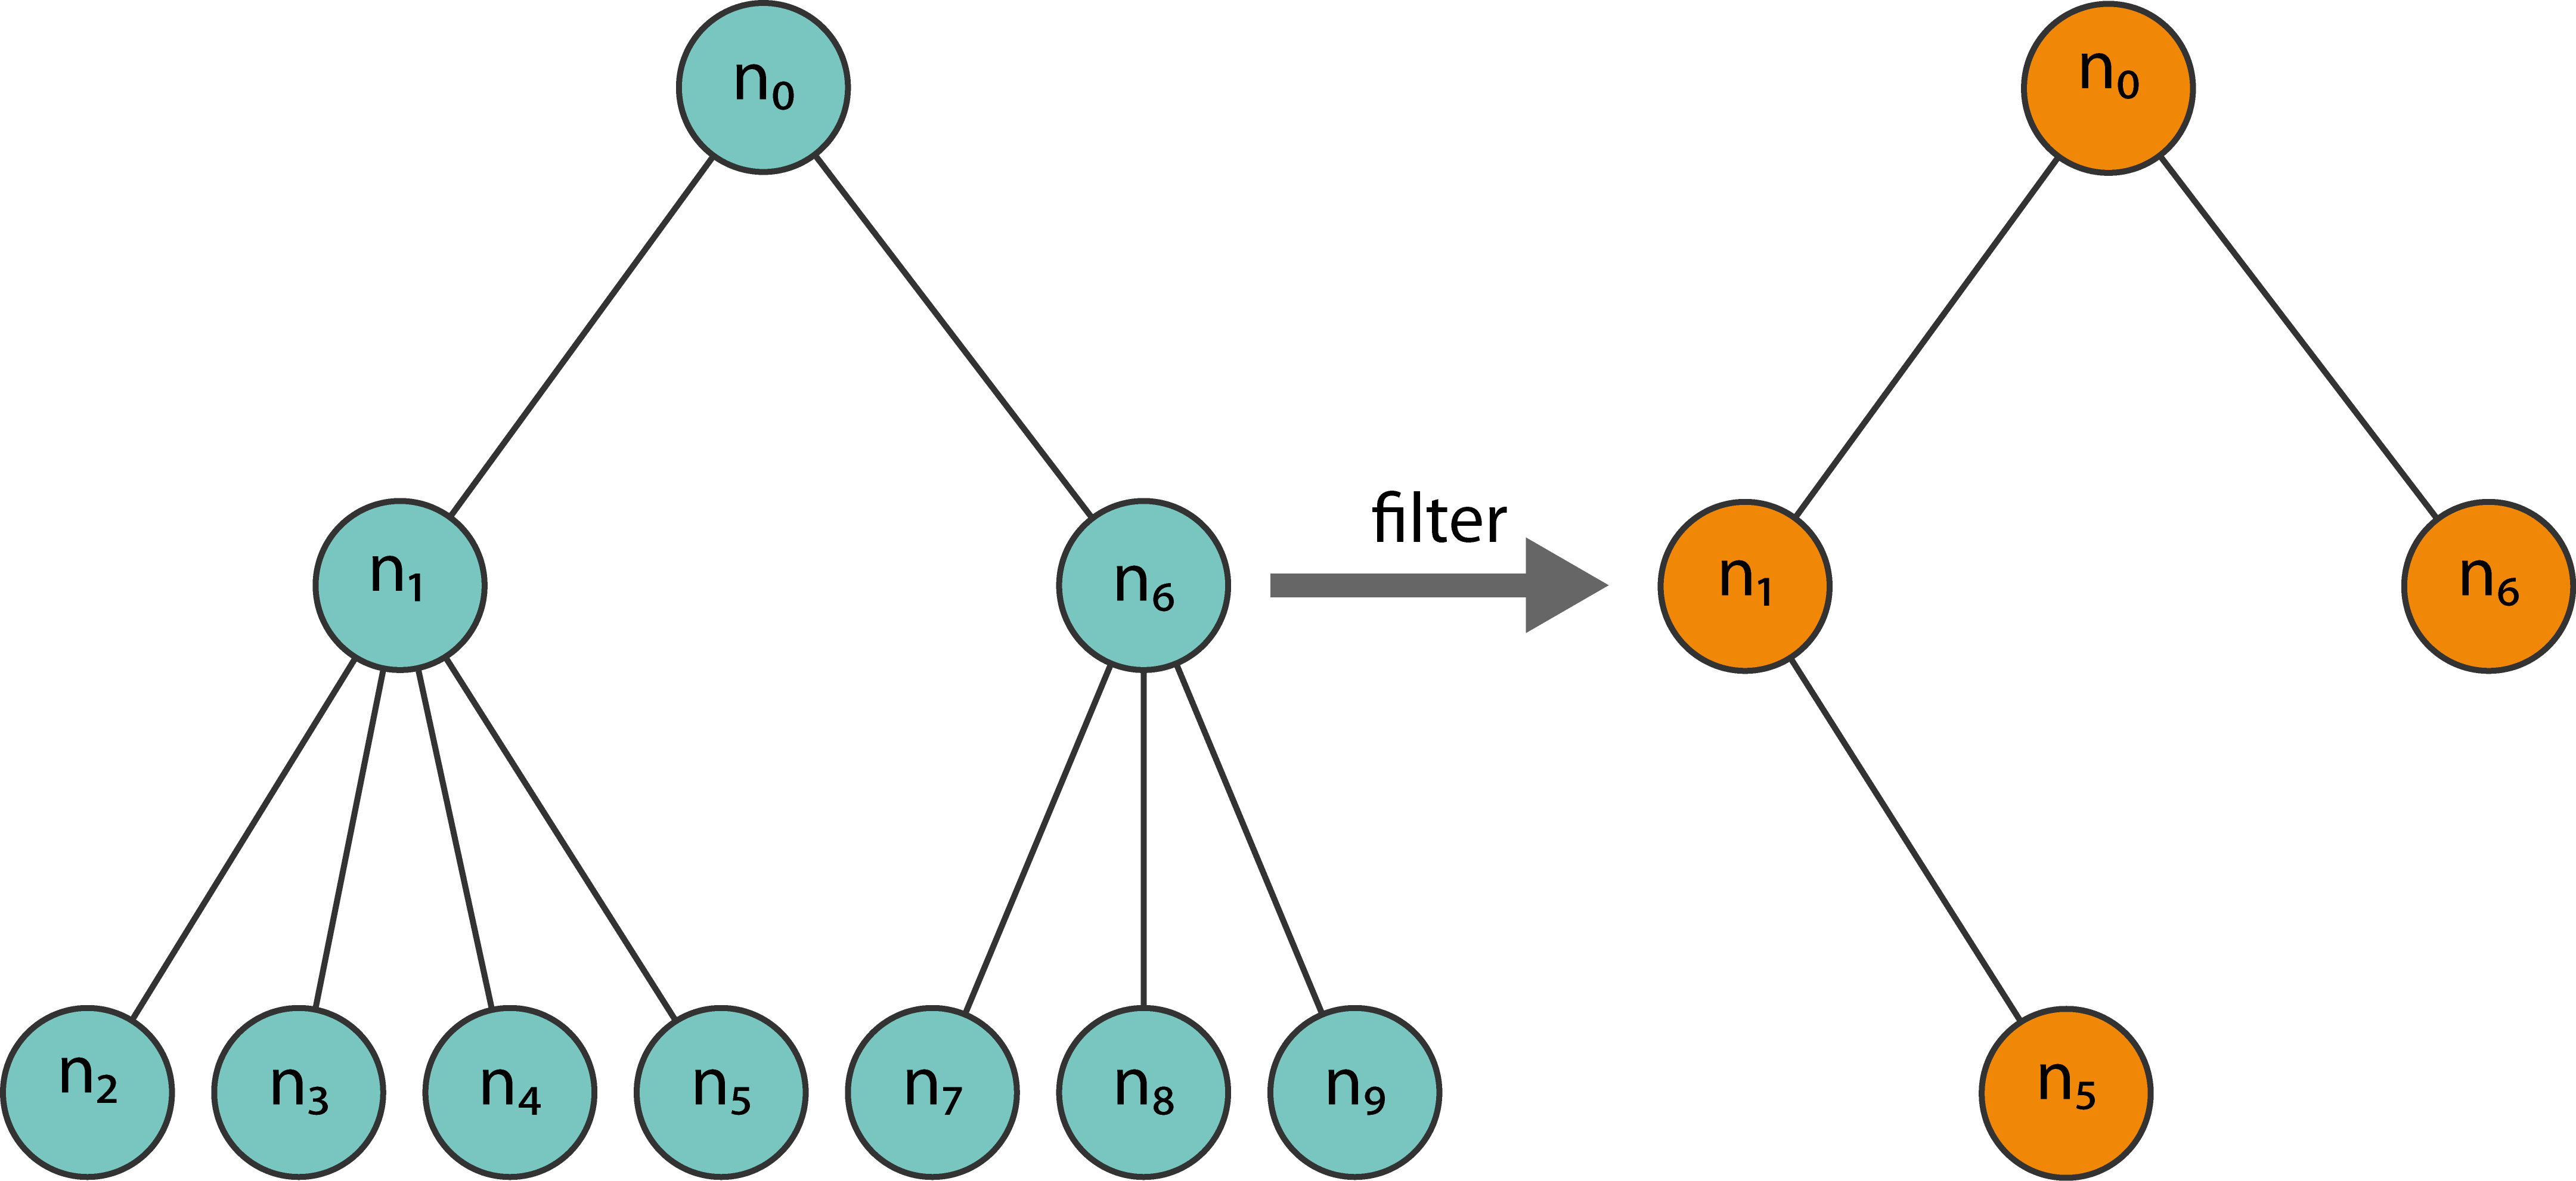
\includegraphics[width=0.55\textwidth]{Implementation/octreeFilter.png}%7
        }\par\medskip
    \subcaptionbox{ \label{fig:octreeMap}}{%
        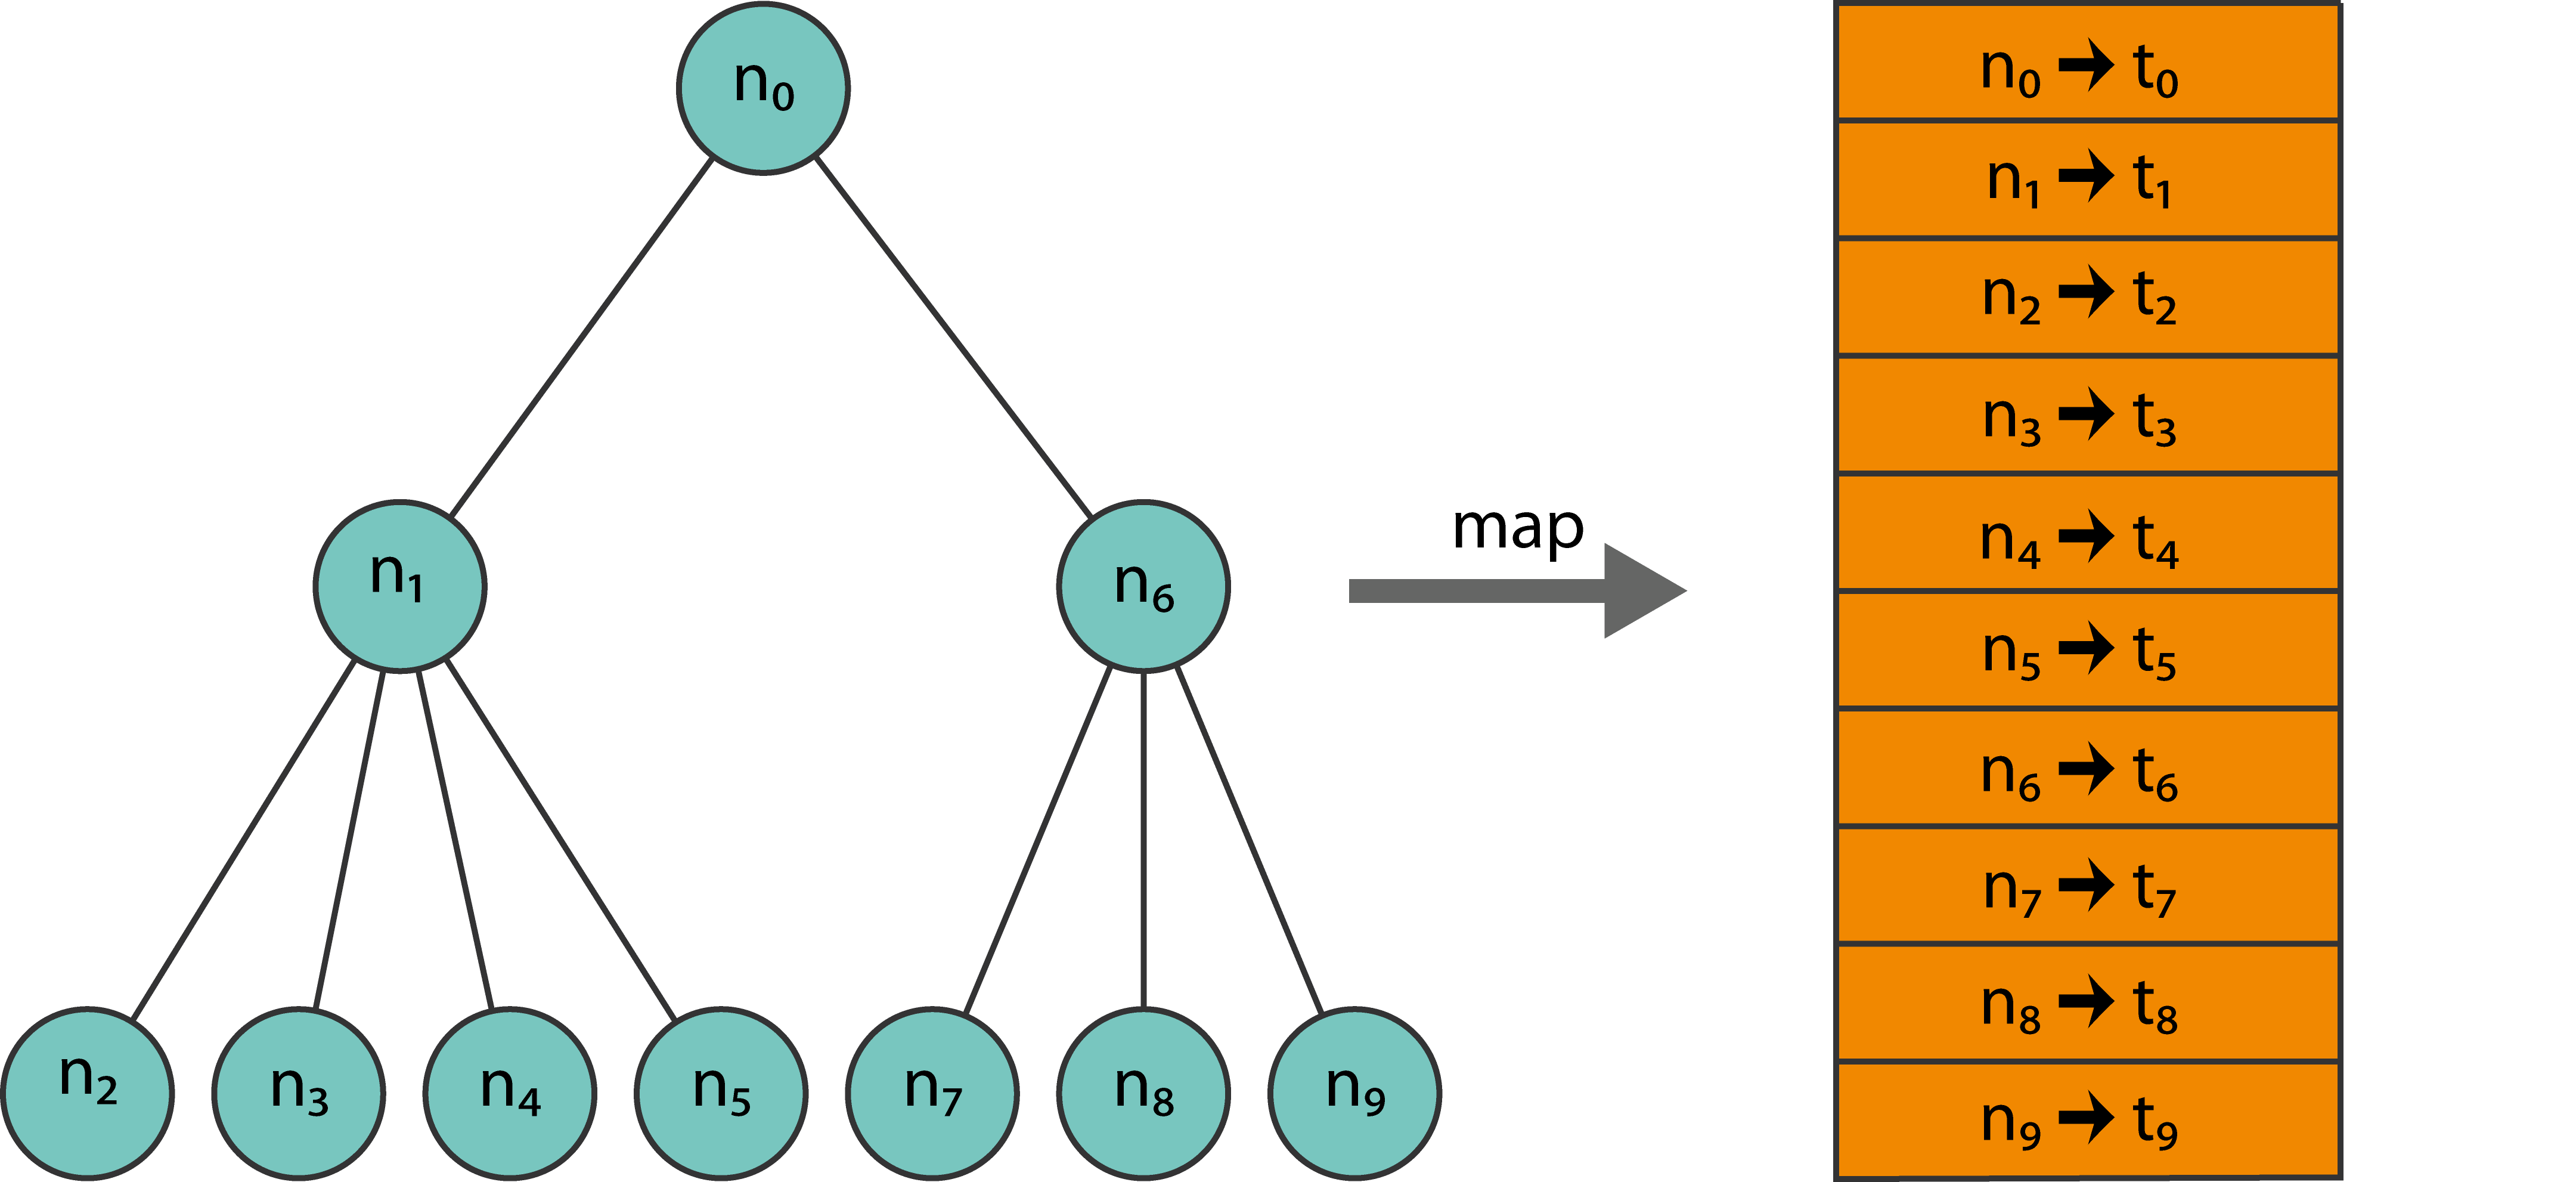
\includegraphics[width=0.55\textwidth]{Implementation/octreeMap.png}%
        }\par\medskip        
    \subcaptionbox{ \label{fig:octreeChoose}}{%
        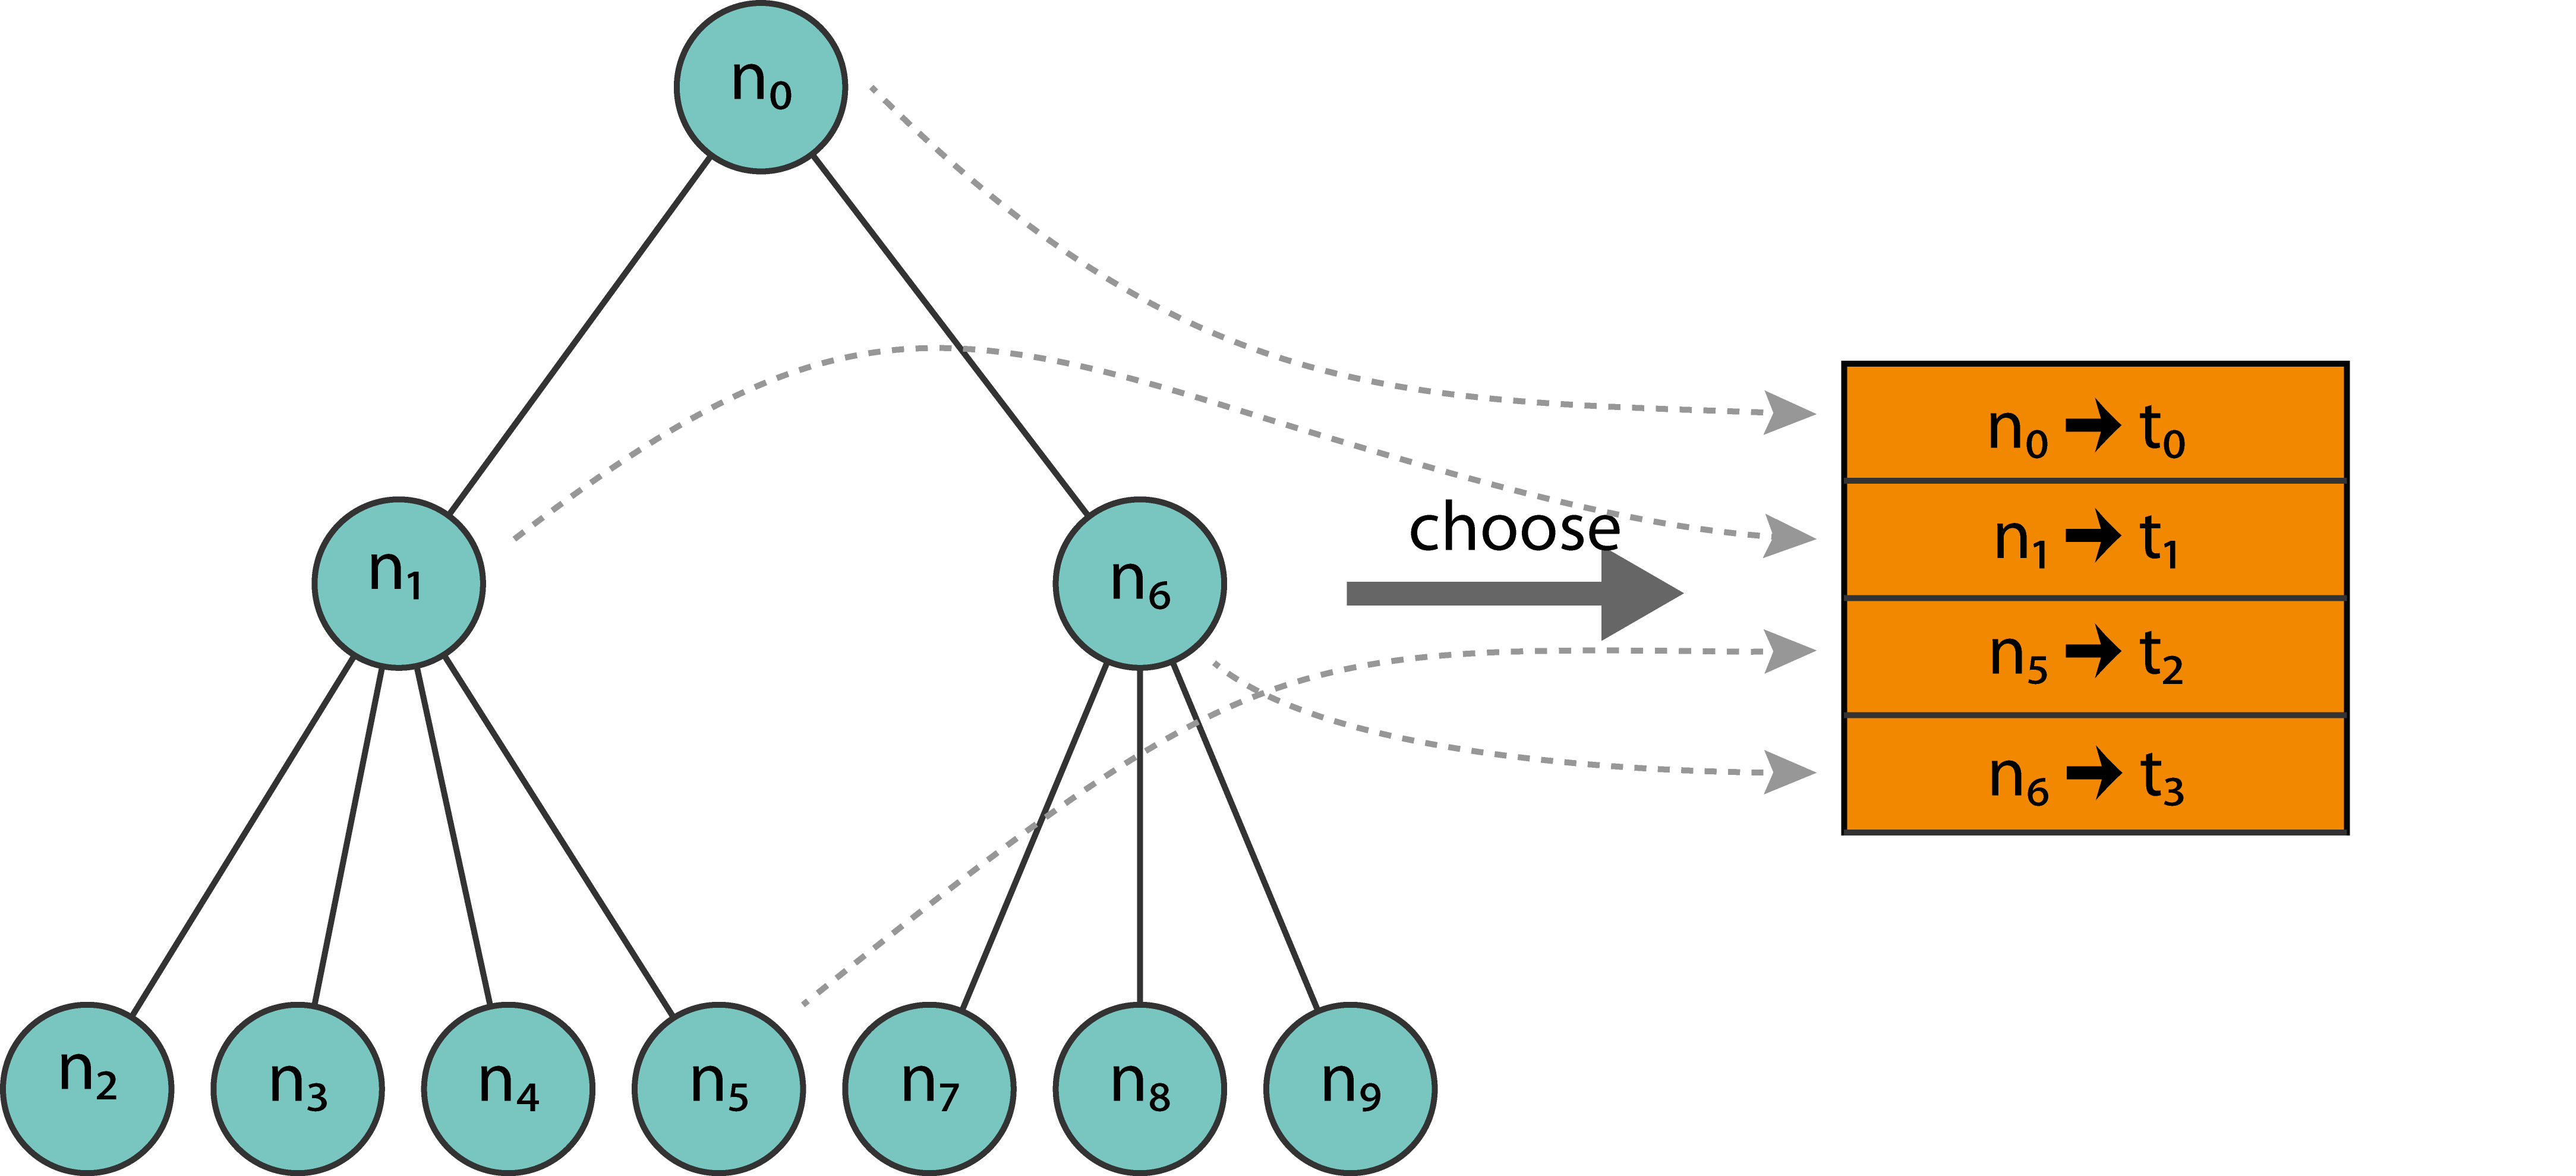
\includegraphics[width=0.55\textwidth]{Implementation/octreeChoose.png}%
        }
    \caption[Filter, map, and choose applied to an exemplary octree]
		{This figure shows an exemplary octree, on which the filter, map and choose function is applied. In (a) the filter function creates a new octree that only contains the nodes that are filtered. (b) shows the result of the map function. Each node in the octree is projected to a new type $t_{i}$ and the result is returned as an array. (c) shows the choose function. Only nodes are returned that fulfill the decision function and are projected to a new type $t_{i}$. }
    \label{fig:octreeFuns}
\end{figure}

Figure \ref{fig:octreeFuns} shows the described functions and their effects on an exemplary octree. The \verb|filter| function returns a new octree, the \verb|map| function returns an array of projected types, the \verb|choose| function is a combination of \verb|filter| and \verb|map| such that only those projections are returned that are of interest. 


\subsubsection{Replacing nodes}

As mutations introduce side effects that can lead to bugs, instead of changing information within an octree node, a new node is created containing the new data. The old node might still be in use in a different thread. Thus, race conditions are possible when mutating values. When information changes in an octree node, a new \verb|thunk| is created that stores the new content onto the disc; the old \verb|thunk| is discarded when it is not used anymore. The newly created node has a distinct position that is determined by the path in the octree. The octree is traversed recursively to find the location of the node. 
When resolving the recursion, the content of all ancestor nodes changes as well, since one of the children is a new node. Therefore, for each ancestor, a new node is created too, containing the new content. Since the root changes as well, as the replaced node is a successor of it, a new octree is constructed each time a node is replaced. This octree, however, contains mostly the data of the old octree, except the replaced node. 

\begin{figure}[h]
    \centering
    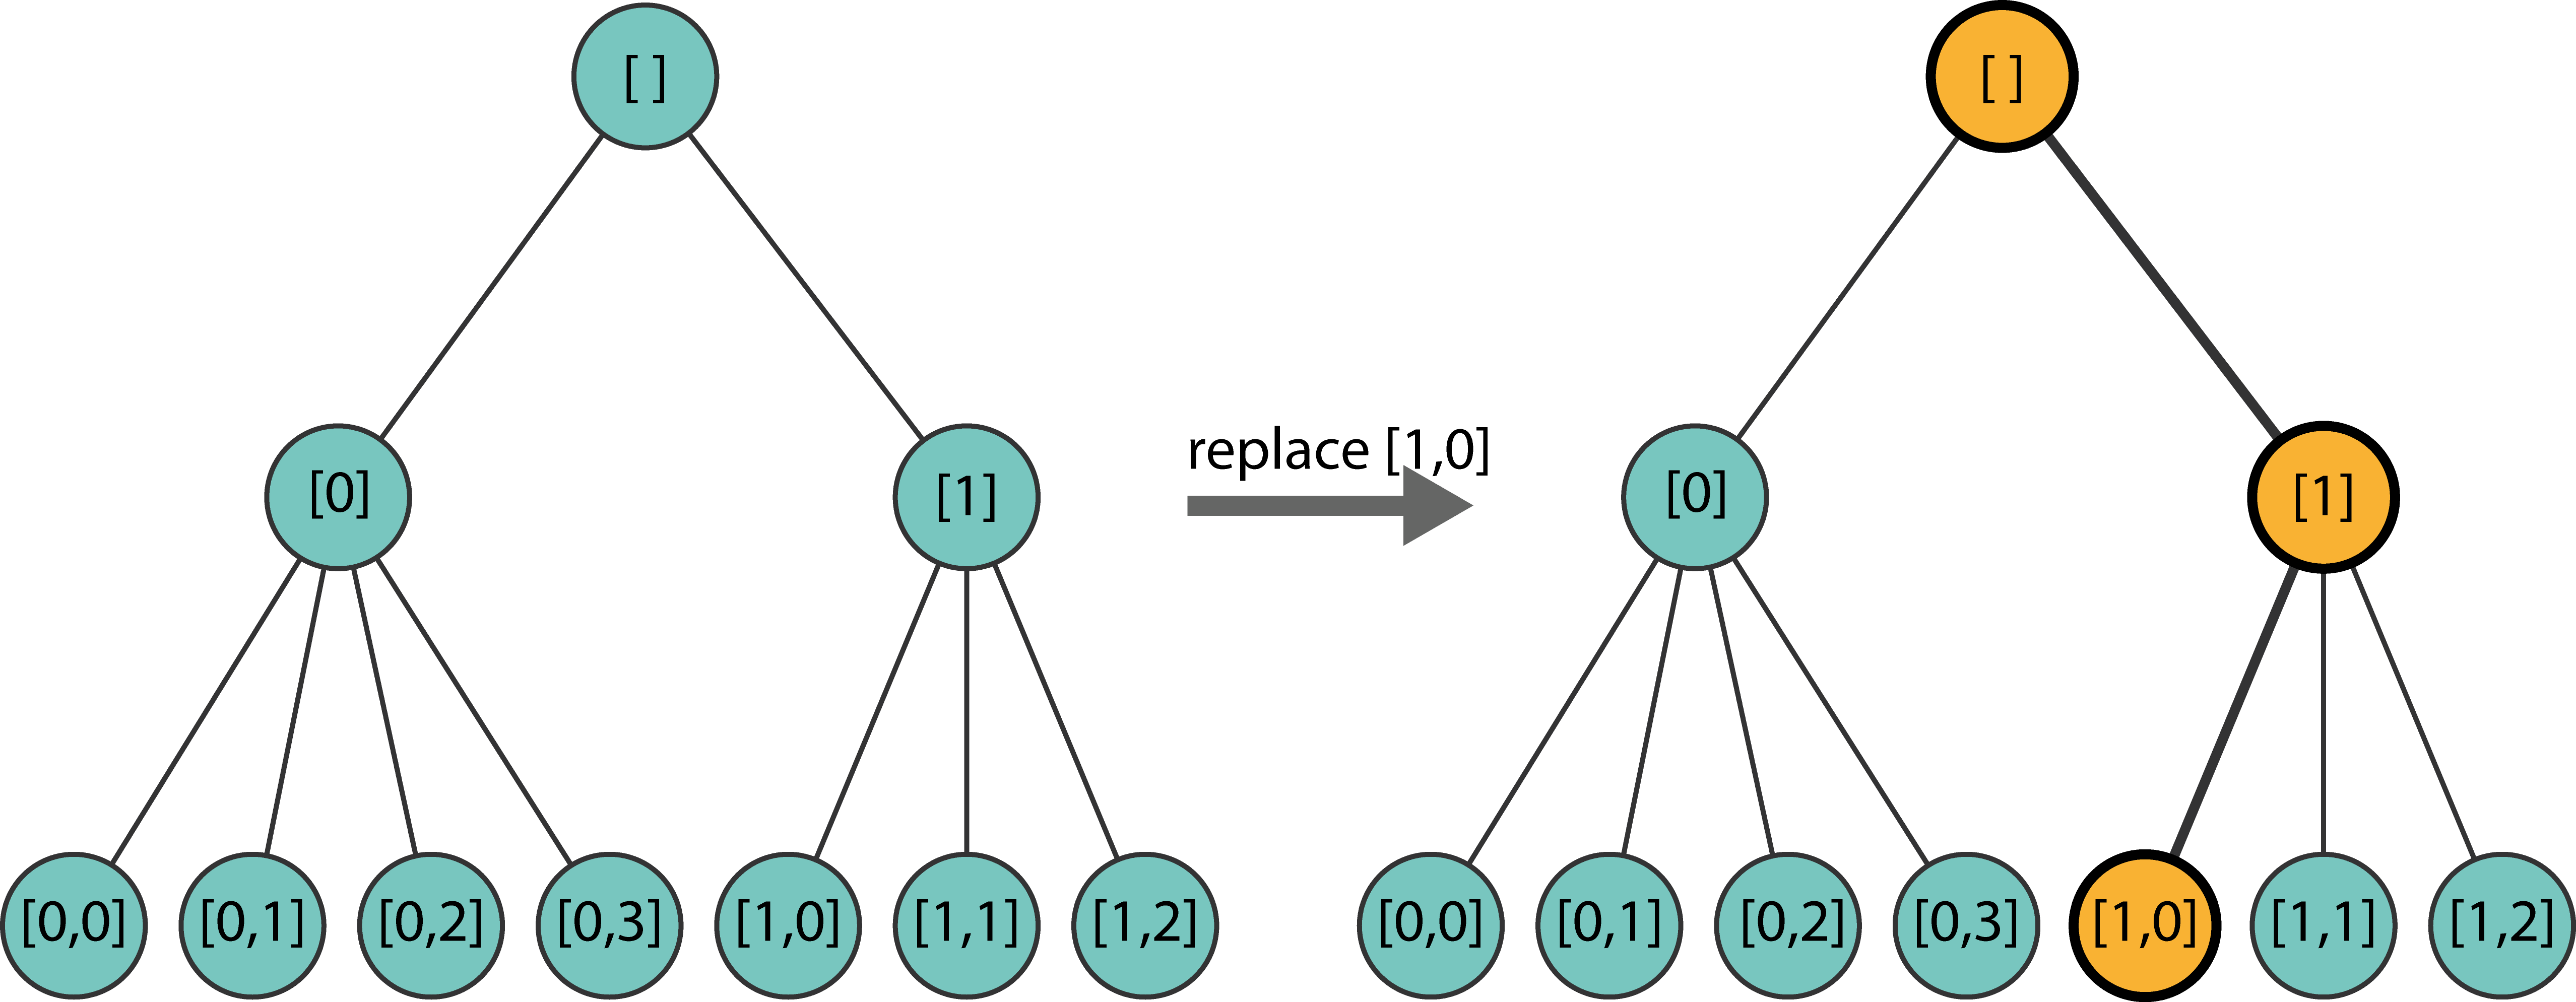
\includegraphics[width=0.8\textwidth]{Implementation/octreeReplace.png}
    \caption[Example on replacing an octree node]
		{Replacing an octree node subsequently changes the node's ancestors as well. The left tree shows the original octree, the right tree is the new octree after the node [1,0] was replaced. The replaced node is highlighted with a red border, all nodes that changed due to the replacement are colored in orange. }
    \label{fig:octreeReplace}
\end{figure}

Figure \ref{fig:octreeReplace} shows an example on the replacement of a node. The nodes are labeled with their paths in the octree to identify them uniquely. The node with label \verb|[1,2]| is replaced. Thus, all ancestors in the octree are changed as well since the node got a new child. Nodes that changed are colored in orange. 


\subsection{Raycast}
Spatial subdivision accelerates ray casting. If the ray does not intersect the bounds of a larger parition of the space, it will not interesect the objects that are contained in the region as well. Thus, large parts of data can be excluded from the ray cast prematurely. The hierarchical structure of the octree ensures that only a minimum set of nodes is tested for intersection. If the ray does not intersect the parent's bounding box, it does not intersect the children's bounding boxes as well. The raycast on the octree can be performed with logarithmic cost. The raycast is implemented using the octree's \verb|choose| function with a decision function that performs the intersection with the bounding box and returns a \verb|RaycastHit| structure containing all necessary information on the raycast hit. 


\subsection{Culling}

Culling utilizes the octree's \verb|filter| function to create a new octree that only contains nodes that are currently rendered. The culling function performs view-frustum culling as well as a level-of-detail culling heuristic based on the node's size and distance to the near plane. Figure \ref{fig:octreeCulling} shows an exemplary culling performed on a tree. The level-of-detail decreases for nodes that are further away from the camera and only those nodes are used that intersect the view frustum.

\begin{figure}
   	\centering
    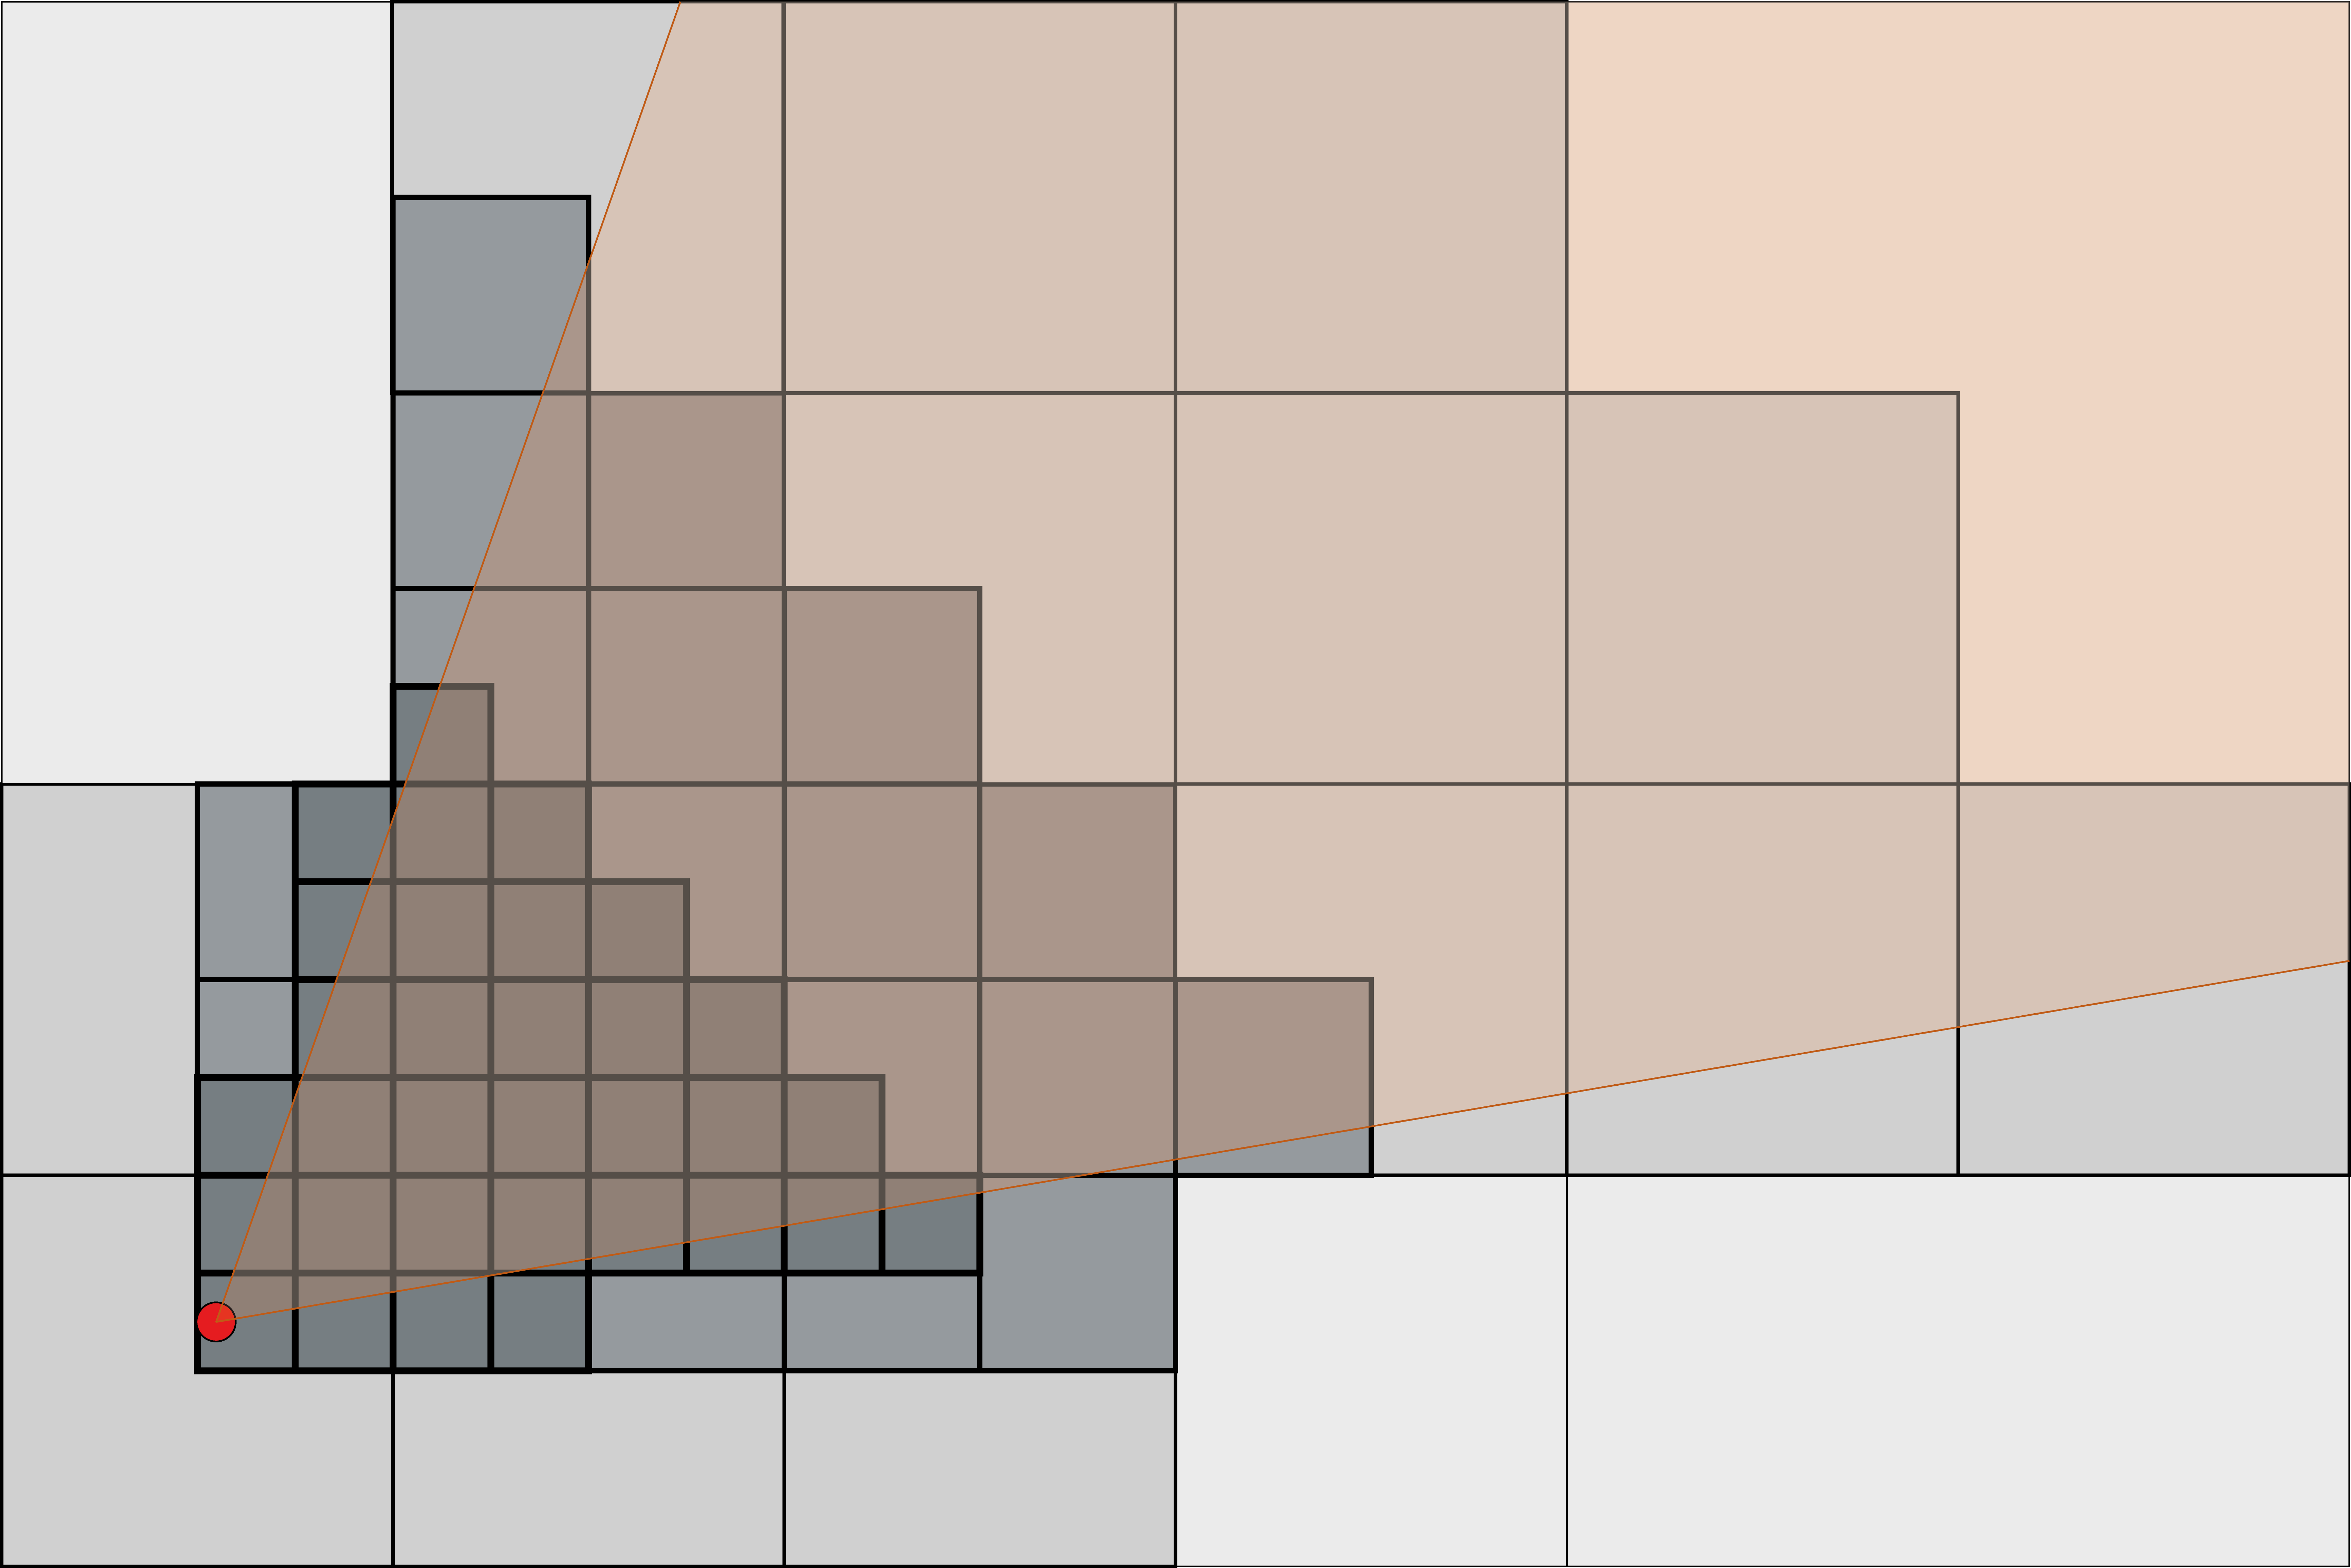
\includegraphics[width=0.8\textwidth]{Implementation/octreeCulling.png}
    \caption[Exemplary octree culling]
		{An exemplary culling is performed on a tree. Octree nodes that are darker with a thicker edge have a higher level-of-detail. Only close to the camera (red), the nodes with the highest level-of-detail are rendered. Nodes that are outside the view frustum (orange) are discarded. }
    \label{fig:octreeCulling}
\end{figure}


Let $V$ be the volume of the node's bounding box, $win_x, win_y$ the dimensions of the window and $d_{min}$ be the smallest distance from the bounding box to the near plane in world space, clamped by the near and far plane. Furthermore, let $t$ be a user-controlled distance threshold. For this application, $t = 2$ is used. 

\begin{center}
$t_{win} = \frac{t}{max (win_x, win_y)}$ \\
$g = \frac{\sqrt[3]{V}}{d_{min}}$ \\
\end{center}
The decision whether or not to render the node is determined by:
\begin{center}
$g > t_{win}$
\end{center}

The user-controlled threshold $t$ is divided by the largest window dimension that allows the level-of-detail to adapt to the window size. $d_{min}$ is calculated by projecting all corners of the node's bounding box to view space and negating the $z$ value. The smallest value is then clamped to the view frustum, so the computation stays in visible view space. A smaller $t_{win}$ allows for higher level-of-detail to be displayed. The granularity $g$ of an octree node is controlled by the minimal distance and the size of the node. Nodes close to the camera have higher granularity. Smaller nodes have smaller granularity. Figure \ref{fig:targetpointDistance} shows the usage of different thresholds $t$ on a point cloud. 

\begin{figure}
    \centering
    \subcaptionbox{ \label{fig:targetpointDistance10}}{%
        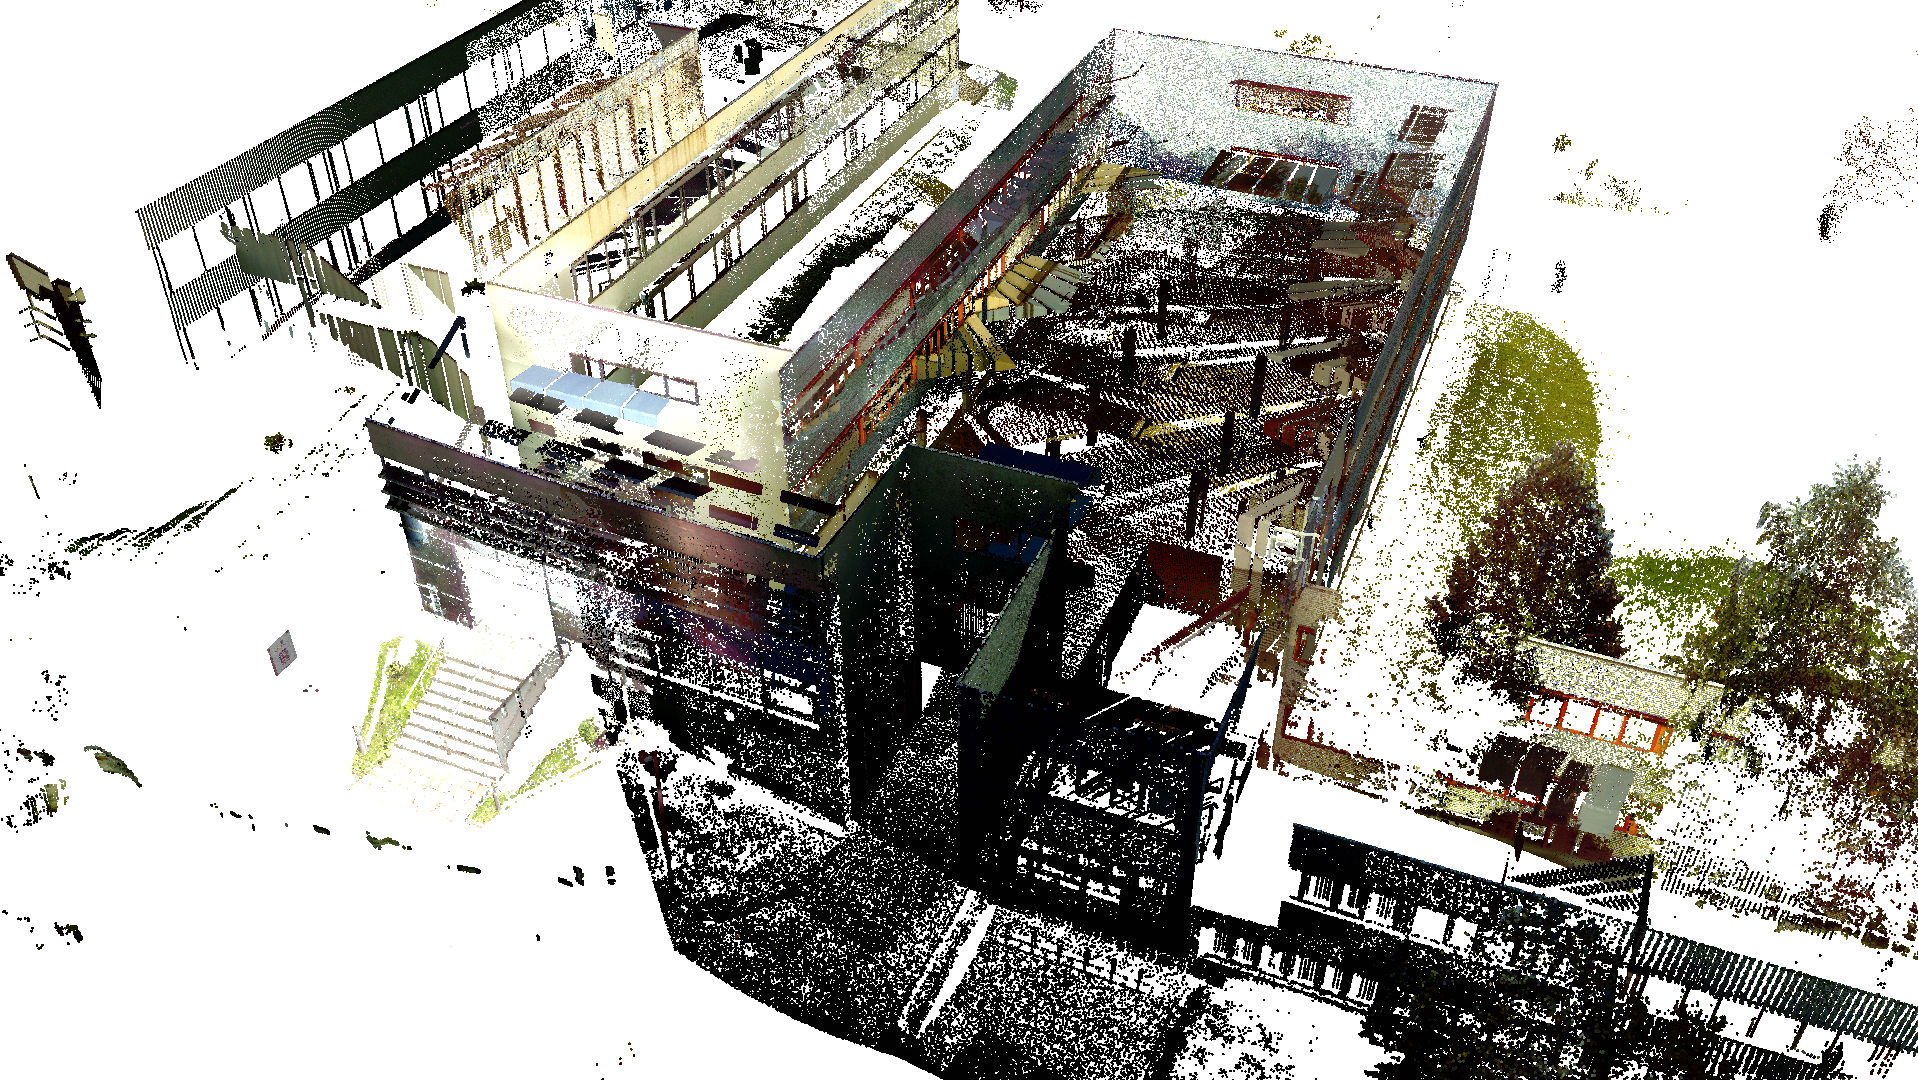
\includegraphics[width=0.6\textwidth]{Implementation/targetpointDistance10.png}%7
        }\par\medskip
    \subcaptionbox{ \label{fig:targetpointDistance25}}{%
        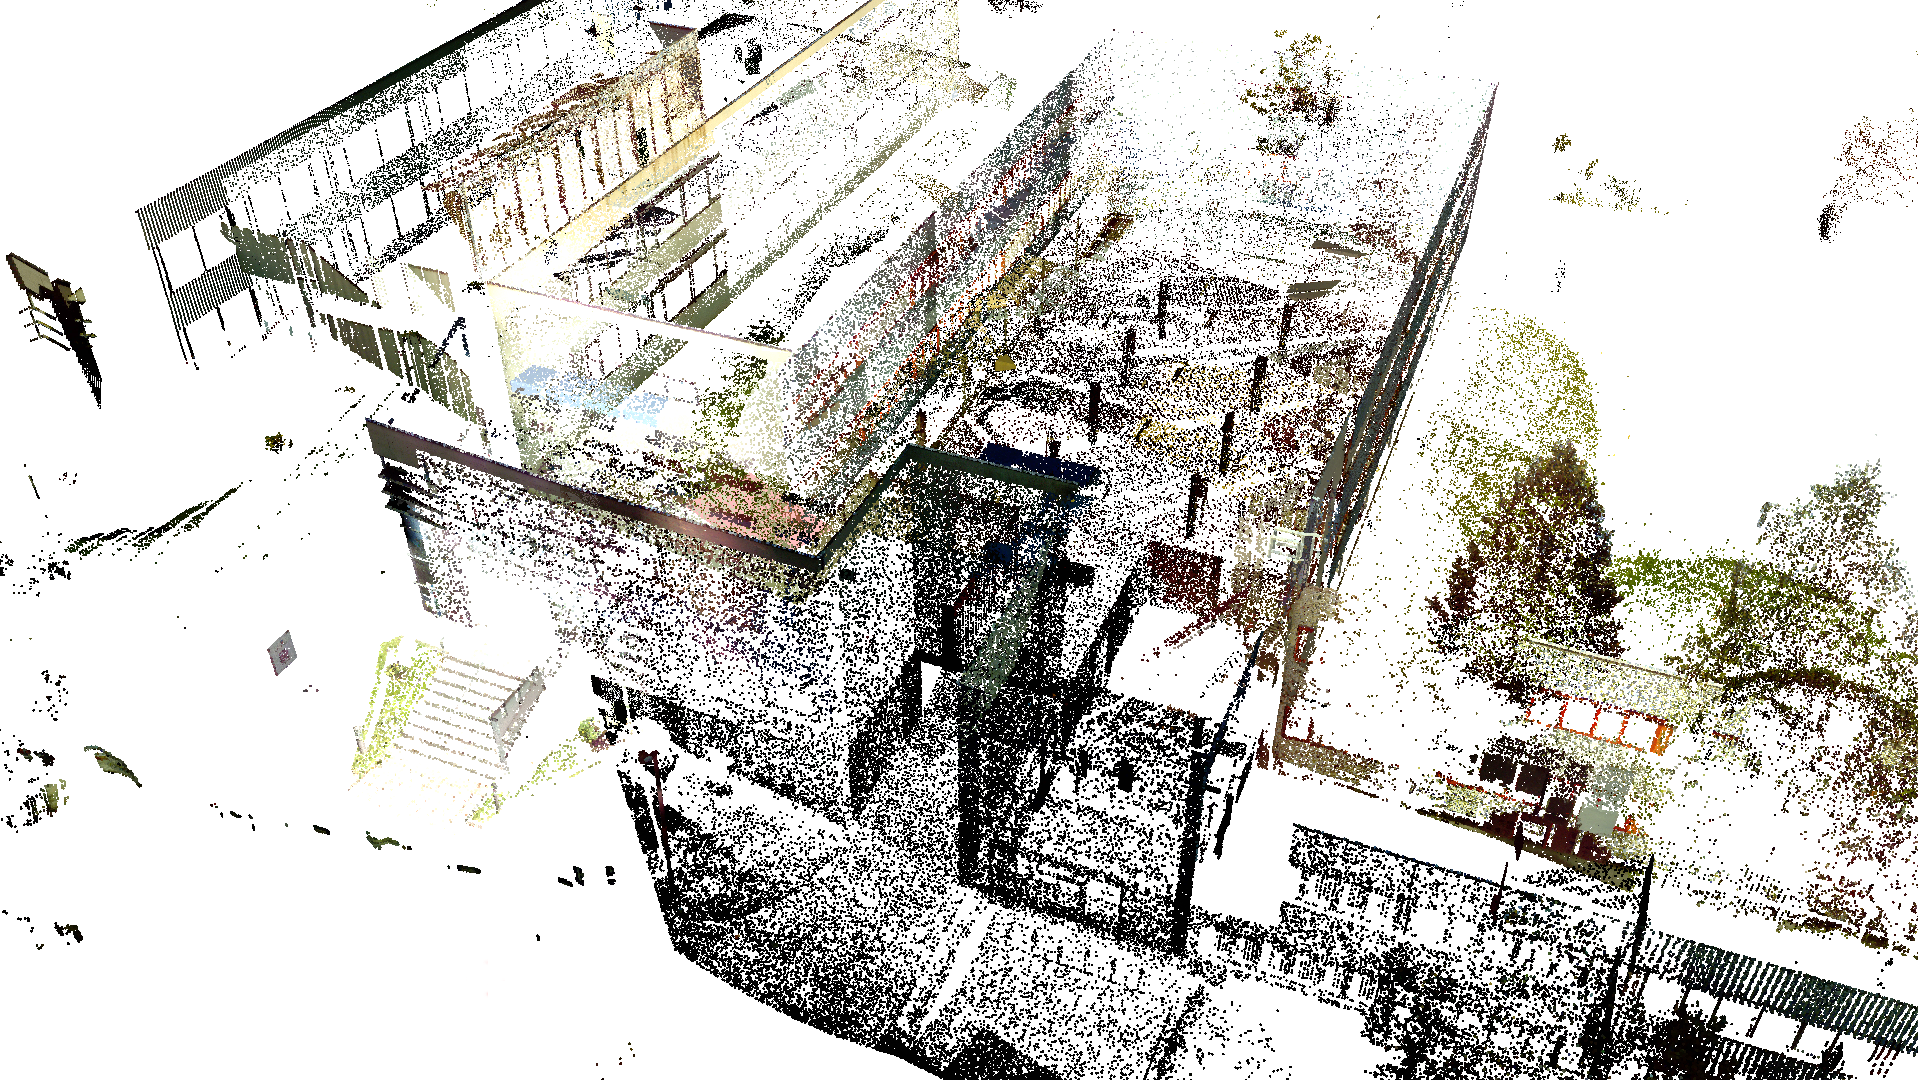
\includegraphics[width=0.6\textwidth]{Implementation/targetpointDistance25.png}%
        }\par\medskip        
    \subcaptionbox{ \label{fig:targetpointDistance50}}{%
        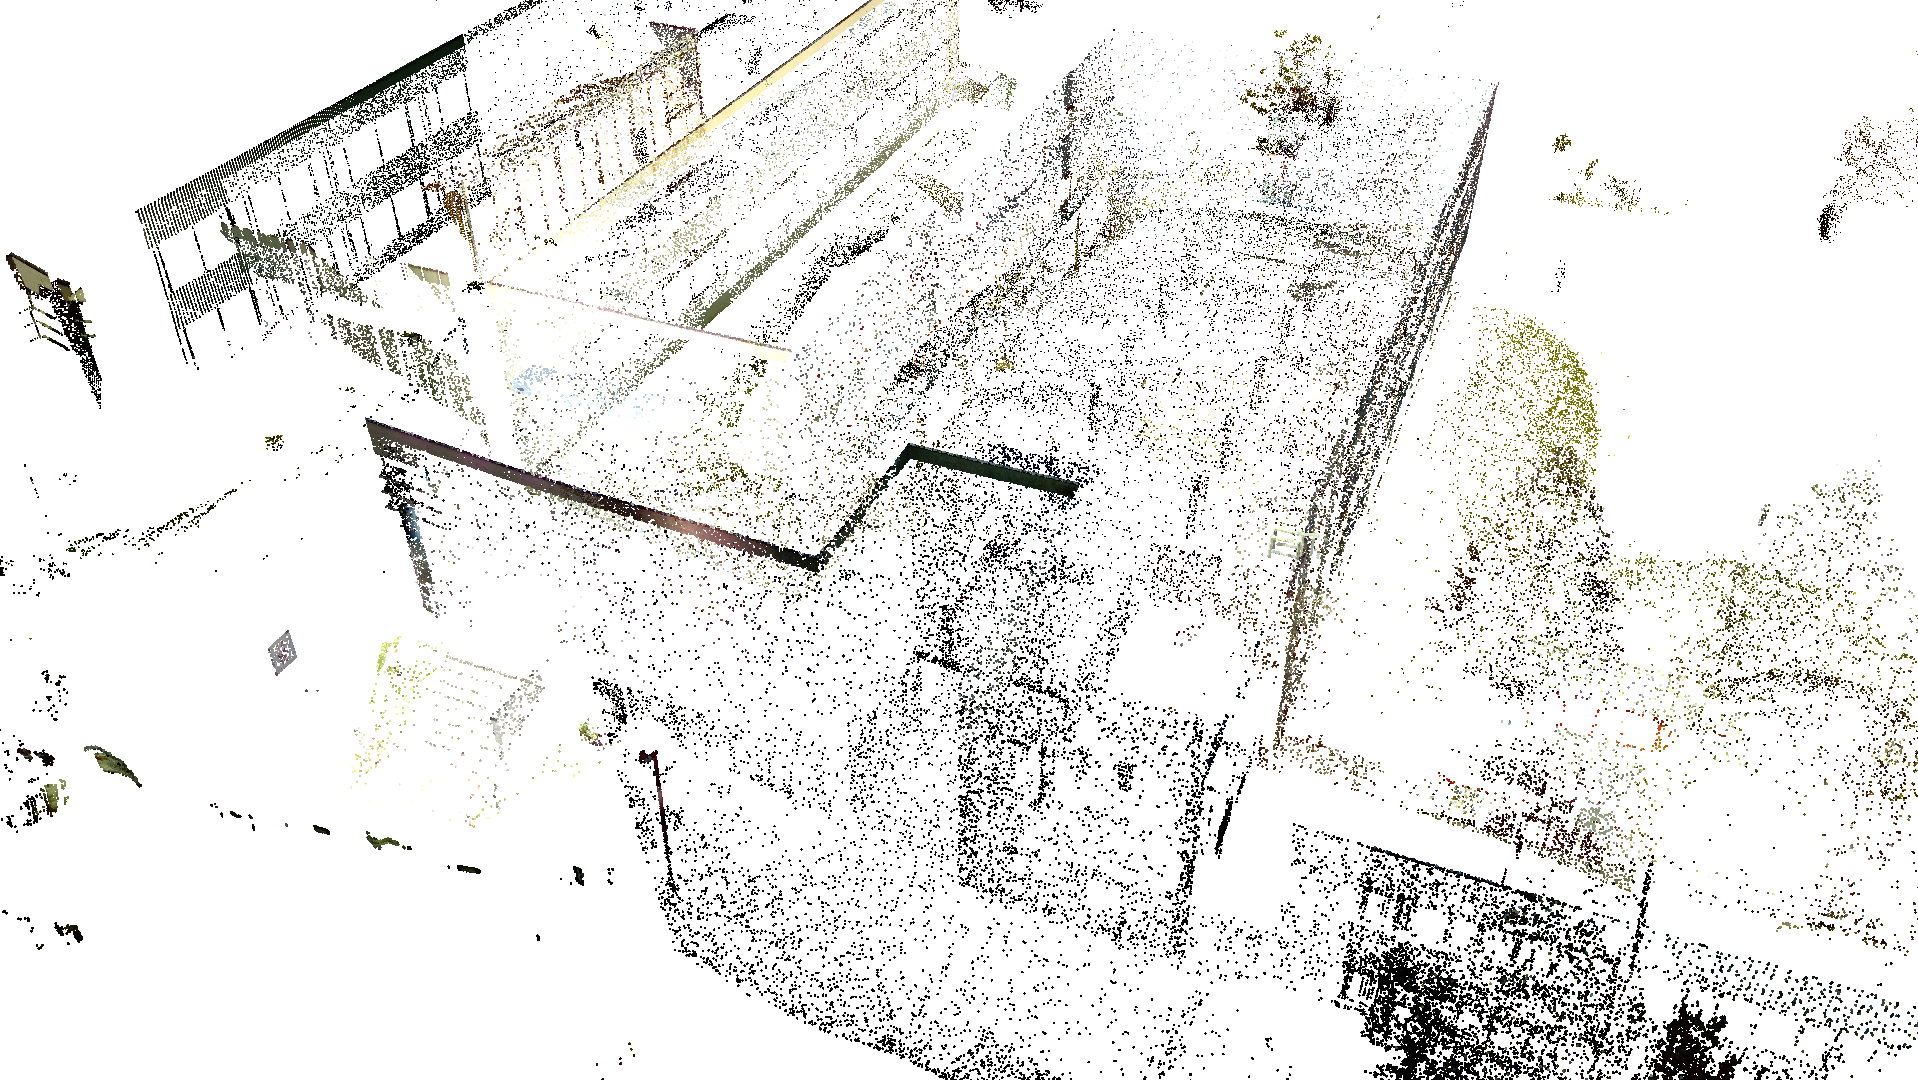
\includegraphics[width=0.6\textwidth]{Implementation/targetpointDistance50.png}%
        }
    \caption[Different $t$ values for Technologiezentrum]
		{This figure shows the Technologiezentrum rendered with a $t$ value of 2, 5, and 10 in (a) - (c). A smaller $t$ results in a more dense visualization of the point cloud for the current view. }
    \label{fig:targetpointDistance}
\end{figure}


\subsection{Diff}

Let $t1, t2$ be two octrees where $t2$ is a sub tree of $t1$ and $v$ a non-negative integer. The function \verb|diff| $t1 t2$ $v$ returns all nodes from $t1$ whose parents exist in $t1$ and $t2$, but the node itself only exists in $t1$. $v$ limits the maximum level-of-detail difference. Hence $v = 1$ only allows for the direct children only, $v = 2$ allows for the children and their children as well. 

\par

The \verb|diff| function takes nodes that are in the first octree and not in the second octree. It comes in two varieties. The first implementation returns only those nodes with the maximum level-of-detail difference. The second implementation returns all intermediate nodes as well. 
The construction of the candidates set for the shape-assisted local level-of-detail increment in Section \ref{sec:lod_increment} is implemented using the \verb|diff| function, where $t1$ is the entire octree, $t2$ is the culled octree that only contains nodes that are rendered and $v$ is the level-of-detail increment parameter.  


\section{Sequential Computation Applicator}

The octree receives changes on a regular basis from multiple sources in this application. The shape detection coroutine continuously inserts detected primitive shapes into the octree, resulting in a new octree every time. User interactions change the point set by selecting regions of interest. To synchronize the octree access, locking mechanics can be used. However, such mechanics can get confusing easily, especially when the application grows. 

\par

All changes to the octree depend on the state of the octree that, in the meantime, may be altered by an operation from a different thread. Furthermore, since a new octree is created every time, the result of an operation may be overwritten by a second operation that starts while the first operation has not yet finished. All subsequent operations depend on the result of the previous operation. Thus, a structure is needed that handles such dependent operations. 

\par

The \textit{sequential computation applicator} is a structure that provides a synchronized way of processing sequential operations. The applicator's functionality is synchronized such that multiple threads can dispatch operations on the octree. The \textit{sequential computation applicator} is a wrapper around a \verb|ModRef<'T>| that invokes changes on this value regularly. 
In this case, the type of the applicator wraps around a \verb|ModRef<Octree>|. 

All dispatched operations are processed sequentially, and the \verb|ModRef|'s value is changed after an operation is completed, thus notifying the Aardvark engine. Since Aardvark evaluates adaptives lazily, operations simply get aggregated as long as no results are requested (i.e., rendering is never stalled). 
The applicator provides the interfaces to dispatch an operation, as well as to dispatch an operation with high priority to enqueue an operation on the front. 

\begin{lstlisting}[language = FSharp]

    member public this.DispatchPrioritized(computation : 'T -> 'T) (timeout : int) (timeoutCallback  : unit -> unit) : unit = ...

    member public this.Dispatch(computation : 'T -> 'T) (timeout : int) (timeoutCallback  : unit -> unit) : unit = ...
   
\end{lstlisting}

The type \verb|'T| is the generic type of the \textit{sequential computation applicator}, in this case, it is \verb|Octree|. A computation is dispatched that takes a \verb|'T|, and projects it to a new \verb|'T| (i.e. all of the previously mentioned computations). The input parameter on execution is the current value of the octree. Additionally, an operation can be shut down after a defined timeout in milliseconds. If this is the case the \verb|timeoutCallback| is invoked to allow clean up and error handling. 


\section{Multi-Threaded Environment}
\label {sec:multithreading}

Multithreading can be achieved on multiple granularities, depending on the task's needs. The application uses three primary threads that run in parallel. The Aardvark rendering engine, combined with the \verb|IMod| evaluation system and user interactions build the main thread of the application. One pitfall of the \verb|IMod| system is that it only reacts to changes in the system, however, to invoke procedures after a particular time without direct changes is not possible since that would involve mutation.

\par

The \textit{user-guided shape detection} in Section \ref{sec:user_guided_sd} is triggered when the camera has not changed for a particular amount of time. As the Aardvark \verb|IMod| system only reacts to changes, such no-changes must be invoked by a separate thread that continuously checks for changes. If a shape detection should be performed, this thread dispatches the computation to the applicator thread.

\par

The \textit{sequential computation applicator} performs changes on the octree. All tasks that are dispatched from multiple threads are executed in a sequential order in the background. The thread transacts the changes to the main thread once a computation has finished. 

\begin{figure}[b]
    \centering
    \includegraphics[width=0.6\textwidth]{Implementation/multiThreading.png}
    \caption[Overview on the multi-threaded environment of the application]
		{The main thread controls the rendering, mod evaluation and interactions. Point selections from interactions are handed to the applicator thread. The shape detection is invoked by a separate thread and dispatched on the applicator thread as well.  }
    \label{fig:multiThreading}
\end{figure}

As Figure \ref{fig:multiThreading} shows, multiple threads are dispatching computations to the applicator thread. However, only this thread transacts changes to the main thread. The shape detection invoker thread works independently of the main thread. 

\par

The second parallelization technique used in this thesis is task-based multithreading. The goal is to identify tasks that are executable in parallel for multiple instances of the same type, such as per-point or per-node computations. As long as shared resources are accessed as read-only, tasks can be executed in parallel without race conditions and the need for locking. The input is an array of elements and a mapping function. The mapping function is executed for each element of the input array using the .Nets \verb|System.Threading.Tasks.Parallel.For| statement. The return type is a new array containing the results of the computation for each element at the original position. The function's signature looks as follows: 

\begin{lstlisting}[language = FSharp]
module Parallel = 
  let map (computation : 'T1->'T2)(array : 'T1[]) : 'T2[]= ...
\end{lstlisting}
The technique is realized as an parallel implementation of F\#s \verb|map| function for arrays. 

\verb|Parallel.map| is used when point or node conversions are needed, such as projecting points to screen space or calculating the distances of points to a shape. 


\section{Point-Cloud Rendering}
\label{sec:rendering}

The culling heuristic described in Section \ref{sec:octree_culling} reduces the octree to set of nodes that can be processed by the GPU and can be drawn in real time. The point data may still be located on the hard drive and must be loaded into memory. 

\par

The Aardvark platform already provides a level-of-detail point cloud rendering system that can handle out-of-core datasets. The rendering system uses a cache to store nodes that were rendered previously. Once a frame is redrawn, all rendered nodes are collected, and for new nodes, the data is loaded into the memory. New nodes are added to the cache, nodes that are not used for this frame, are kept in the cache until the memory consumption requires removal of unused data. For each node new to the cache, a queue entry is added for a worker thread to load the point data into memory, stored in a working set. This working set reacts to changes like an \verb|IMod| so that every time a new entry is created, re-evaluation is triggered and a frame is drawn. Thus, the point-cloud data that is loaded into memory appears gradually on the screen. 

\par

Mathematically, a point has no extent. Therefore it cannot be depicted directly. A common way to draw points is to interpret them as splats of certain size and shape. In this thesis, the points are represented by a sphere imposter. For each point, a camera-aligned quad is created in a geometry shader, whose size is the diameter of the sphere, pixels that are outside the radius of the sphere are discarded. 

\par

Popping effects occur when the view changes and overlapping impostors change their order. Similar to the approach by Schütz and Wimmer \cite{SCHUETZ-2015-HQP}, each splat is given a depth displacement that mimics a sphere's curvature. The splat is extruded towards the camera with a depth value dependent on the distance to the splat's center. This displacement causes the impostors to intersect naturally, thus reducing depth-related popping effects. Figure \ref{fig:point_sprites} shows a direct comparison of using spheres and circular splats. 


\begin{figure}
\centering
\subcaptionbox{ \label{fig:point_circles}}{%
  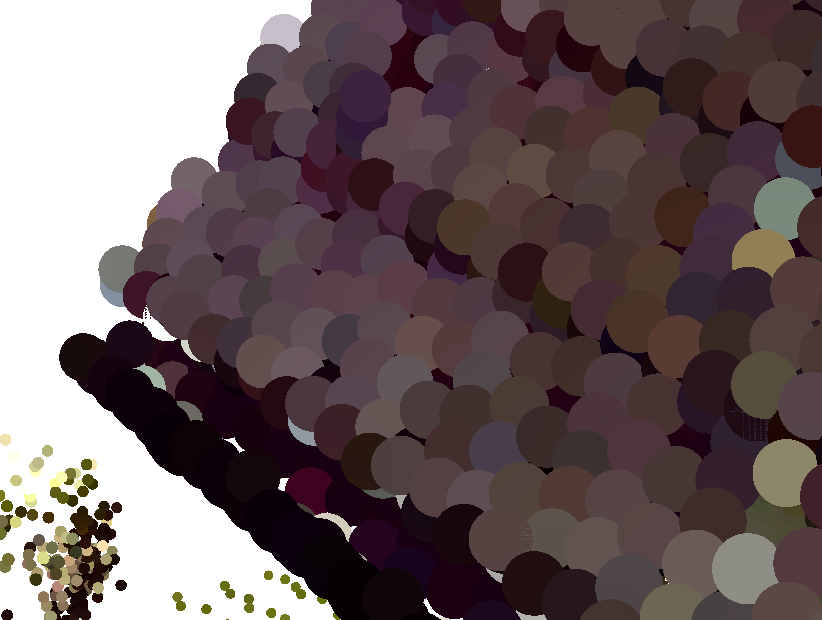
\includegraphics[width=0.48\textwidth]{Implementation/pointCircles.png}%7
  }
\subcaptionbox{ \label{fig:point_spheres}}{%
  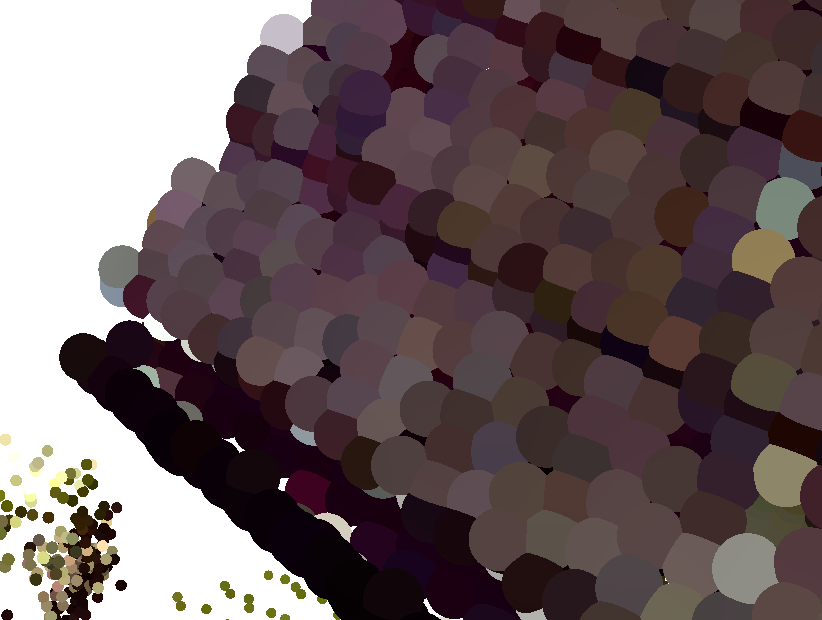
\includegraphics[width=0.48\textwidth]{Implementation/pointSpheres.png}%
  }
  
\caption[Comparison of (a) circular splats and (b) sphere impostors]
{This figure shows a direct comparison of using (a) circular splats and (b) sphere impostors with depth displacement. In (b) the intersections between points are visible due to the spherical shape, whereas points that are a little below other points are occluded almost entirely.}
\label{fig:point_sprites}
\end{figure}
\chapter{Results}
\label{chap:results}


All results are obtained on a PC with an AMD FX-9590, 16 GB RAM and an AMD Radeon HD 7970. The datasets Technologiezentrum and JB\_Haus are a courtesy of rmData\cite{rmdata}. Section \ref{sec:shape_detection_results} shows benchmarks for the shape detection and verifies the capability of the user-guided shape detection to be performed in interactive time. Section \ref{sec:interaction_results} provides a set of screenshots that show the workflow of the user-guided interactions on a different data set. 


\section{Shape Detection Results}
\label{sec:shape_detection_results}
The interactions proposed in this thesis heavily rely on the ability to detect meaningful shapes for regions of interest within interactive time. Therefore it must be assured that the shape detection provides results within interactive time such that the detected shapes can be used immediately for interactions. Section \ref{sec:shape_detection_performance} discusses the performance obtained in the test computer. 


\subsection{Performance}

\label{sec:shape_detection_performance}

The goal of the \textit{user-guided shape detection} is to provide meaningful results within interactive time, such that detected shapes can be used to support interactions immediately. The capabilities of the implementation by Schnabel et al. \cite{schnabel-2007-software} are benchmarked on three different datasets: 

\begin{center}
\begin{tabular}{ l | r | r | r }
                                                                & \textbf{\#Points}             & \textbf{\#Nodes} & \textbf{max. LoD} \\
    \hline
  JB\_Haus.pts                                    & 620.722                                 & 440             & 15 \\
  Technologiezentrum\_Teil1.pts    & 11.762.924                            & 8863             & 15 \\
  Synthetic\_Primitives.pts         & 472.000                                 & 315                 & 5 \\
    
\end{tabular}
\end{center}

The tests are performed without user interaction. Instead, all octree nodes are collected and fed into the shape detection routine sequentially to retrieve results for each node of the point cloud. Therefore, the shape detection is performed for the complete point cloud for each \textit{level-of-detail}. Each octree node contains at most 5000 points. The results are averaged over five runs. Table \ref{table:schnabel_benchmarks} shows the results averaged over all nodes. It can be seen that detecting planes only is significantly faster than detecting all types of primitive shapes. However, detecting all types of primitive shapes still produces results within interactive time. The synthetic point cloud is constructed from a set of primitives that are discretized to point sets, such that all types of primitives exist. 

\begin{table}
    \centering
    \begin{tabular}{ l || r | r | r || r | r | r}
            &\multicolumn{3}{c||}{\textbf{\#Shapes}} & \multicolumn{3}{c}{\textbf{Time (s)}}\\
            &\textbf{min} & \textbf{max} & \textbf{avg}  & \textbf{min} & \textbf{max} & \textbf{avg}  \\
            \hline
            JB\_Haus*                            & 0 & 6  & 1.31 & 0.000026 & 0.578664 & 0.022396 \\
            JB\_Haus                             & 0 & 6  & 1.40 & 0.000024 & 0.741384 & 0.093264 \\
            Technologiezentrum*        & 0 & 10 & 1.18 & 0.000023 & 0.440614 & 0.018781 \\
            Technologiezentrum         & 0 & 10 & 1.19 & 0.000024 & 0.991554 & 0.083180 \\
            Synthetic*                        & 0 & 7  & 1.89 & 0.000026 & 0.440064 & 0.029779 \\
            Synthetic                         & 0 & 7  & 1.24 & 0.000024 & 0.753345 & 0.136474 \\
        \end{tabular}
    \caption{Performance measures for the different datasets averaged over all nodes. The number of shapes and duration are listed as minimum, maximum and average. Each dataset is benchmarked using plane detection only (items with *), as well as detecting all types of primitive shapes. }
    \label{table:schnabel_benchmarks}
\end{table}


\begin{figure}[h]
    \centering
    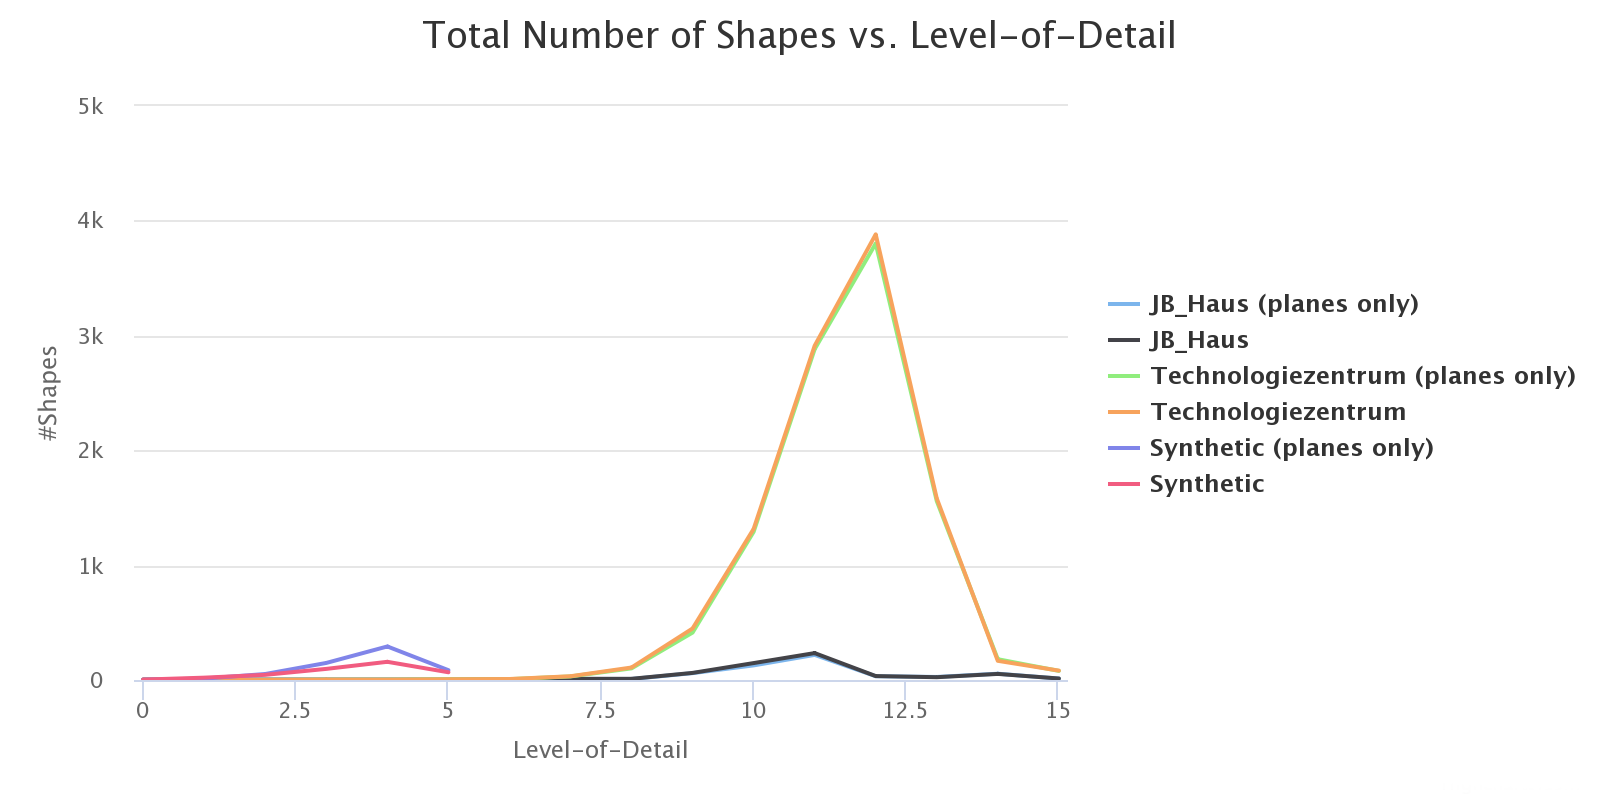
\includegraphics[width=1\textwidth]{Results/shapes_total_vs_lod.png}
    \caption{Plot of the number of shapes in correlation to the \textit{level-of-detail} of the node. All values are averaged over all nodes that share the same \textit{level-of-detail}.}
    \label{fig:shapes_total_vs_lod}
\end{figure}

\begin{figure}[h]
    \centering
    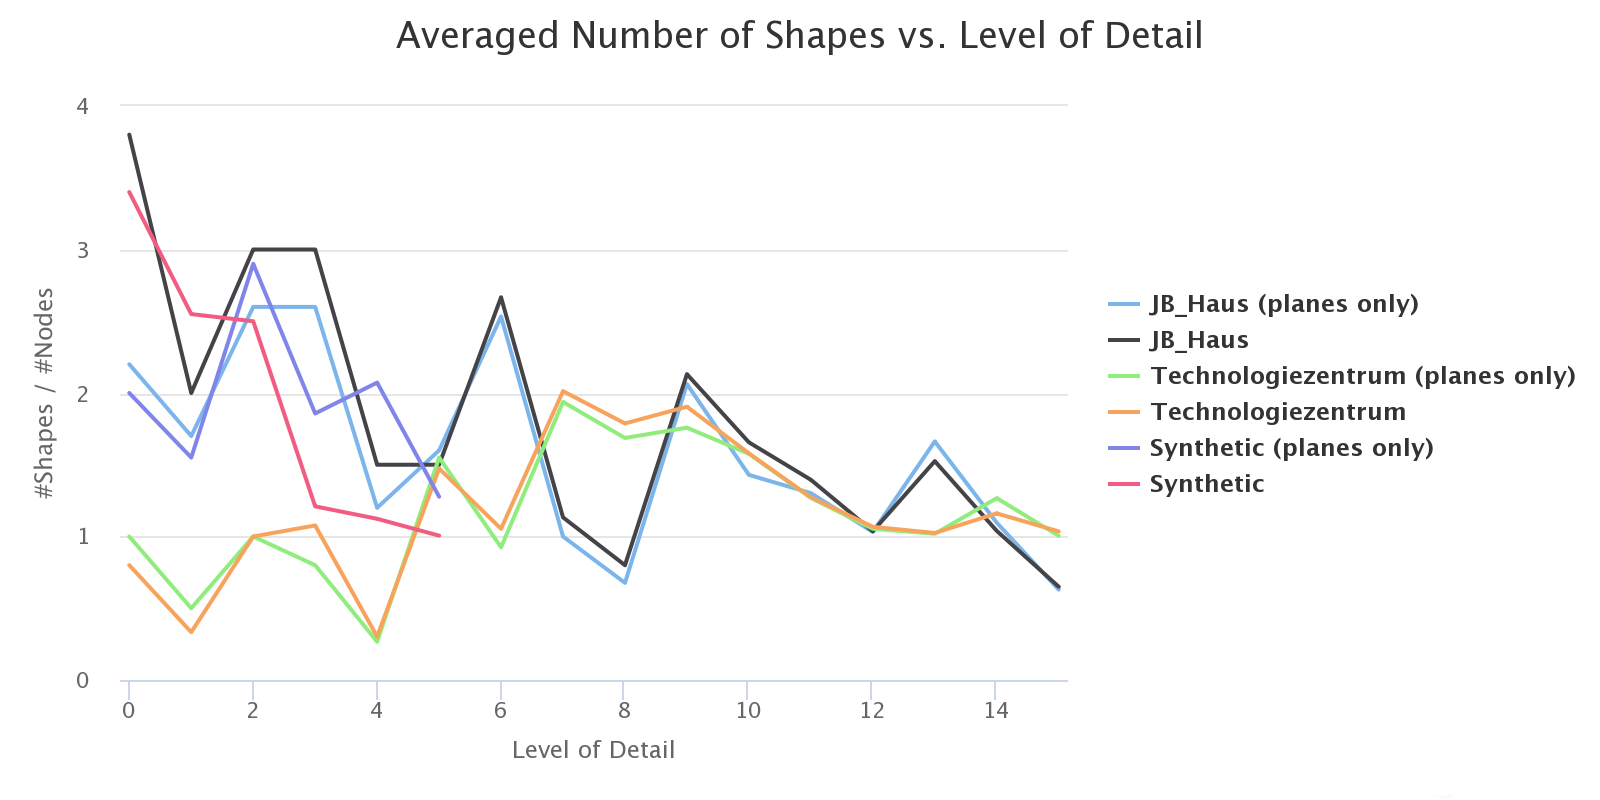
\includegraphics[width=1\textwidth]{Results/shapes_averaged_vs_lod.png}
    \caption{Plot of the number of shapes in correlation to the \textit{level-of-detail} of the node. All values are averaged over all nodes that share the same \textit{level-of-detail}.}
    \label{fig:shapes_averaged_vs_lod}
\end{figure}

\begin{figure}[h]
    \centering
    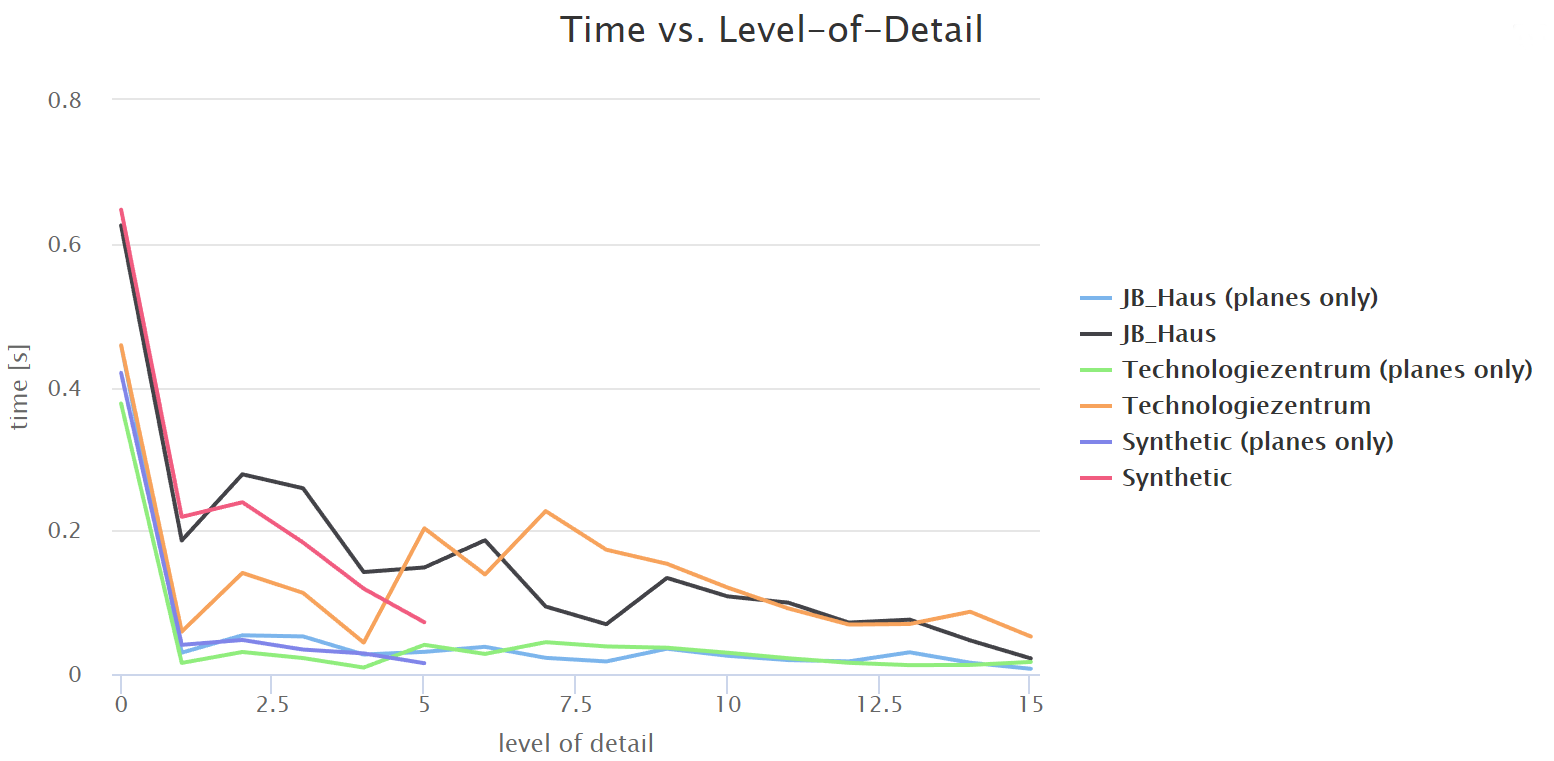
\includegraphics[width=1\textwidth]{Results/time_vs_lod.png}
    \caption{Plot of the number of shapes in correlation to the \textit{level-of-detail} of the node. All values are averaged over all nodes that share the same \textit{level-of-detail}.}
    \label{fig:time_vs_lod}
\end{figure}


Figure \ref{fig:shapes_total_vs_lod} shows the total number of shapes per \textit{level-of-detail}. All three datasets share increase in the number of shapes in the third quarter before a rapid decline for the highest \textit{level-of-detail}. Figure \ref{fig:shapes_averaged_vs_lod} shows the number of shapes divided by the number of nodes per \textit{level-of-detail}. Both figures emphasize that the majority of shapes is not found in the highest \textit{level-of-detail}. Reasons for this is that many nodes only contain a handful of points or only contain a single structure. 
\\

Figure \ref{fig:time_vs_lod} shows the calculation time compared to the \textit{level-of-detail}. Shape detection for smaller, more dense nodes take less time than for larger nodes with lower \textit{level-of-detail} as in larger nodes, usually more shapes are found. 


\subsection{Problems and undesired Behavior}

A problem with the shape detection implementation by Schnabel et al. \cite{schnabel-2007-software} are reoccurring non-terminations for some octree nodes, causing the shape detection coroutine to stall. To circumvent this problem, all shape detection tasks that are dispatched to the \verb|sequential computation applicator| are assigned a timeout value of one second, after which the computation is interrupted. 
\\
Another reoccurring problem with the shape detection is the plausibility of detected shapes. The RANSAC options guarantee that shapes are found that fit the local geometry within a certain margin, $\alpha$ for the normal's angle and $\epsilon$ for the distance the shape. So within theses two parameters, the shape is considered to be valid. However, certain constellations of points allow the shape detection to produce non-plausible results that are accurate regarding the RANSAC parameters but are not plausible to the eye. A prominent example is a torus that is fitted onto a section that describes a cylinder. The major radius of the torus is of such dimensions that the local cylinder fits within the curvature of the torus. Thus, a torus is detected, rather than the simpler cylinder. Figure \ref{fig:missfittedTorus} shows this behavior within an example scene that consists multiple primitives. Figure \ref{fig:missfittedTorus2} shows the size of the detected torus. 
\\
Such non-plausible shapes can exist due to the density-controlled $\epsilon$ parameter that weakens the margin for octree nodes of larger volume. Even within a node, the density can strongly vary for different regions. 

\begin{figure}[h]
\centering
\subcaptionbox{ \label{fig:missfittedTorus1}}{%
  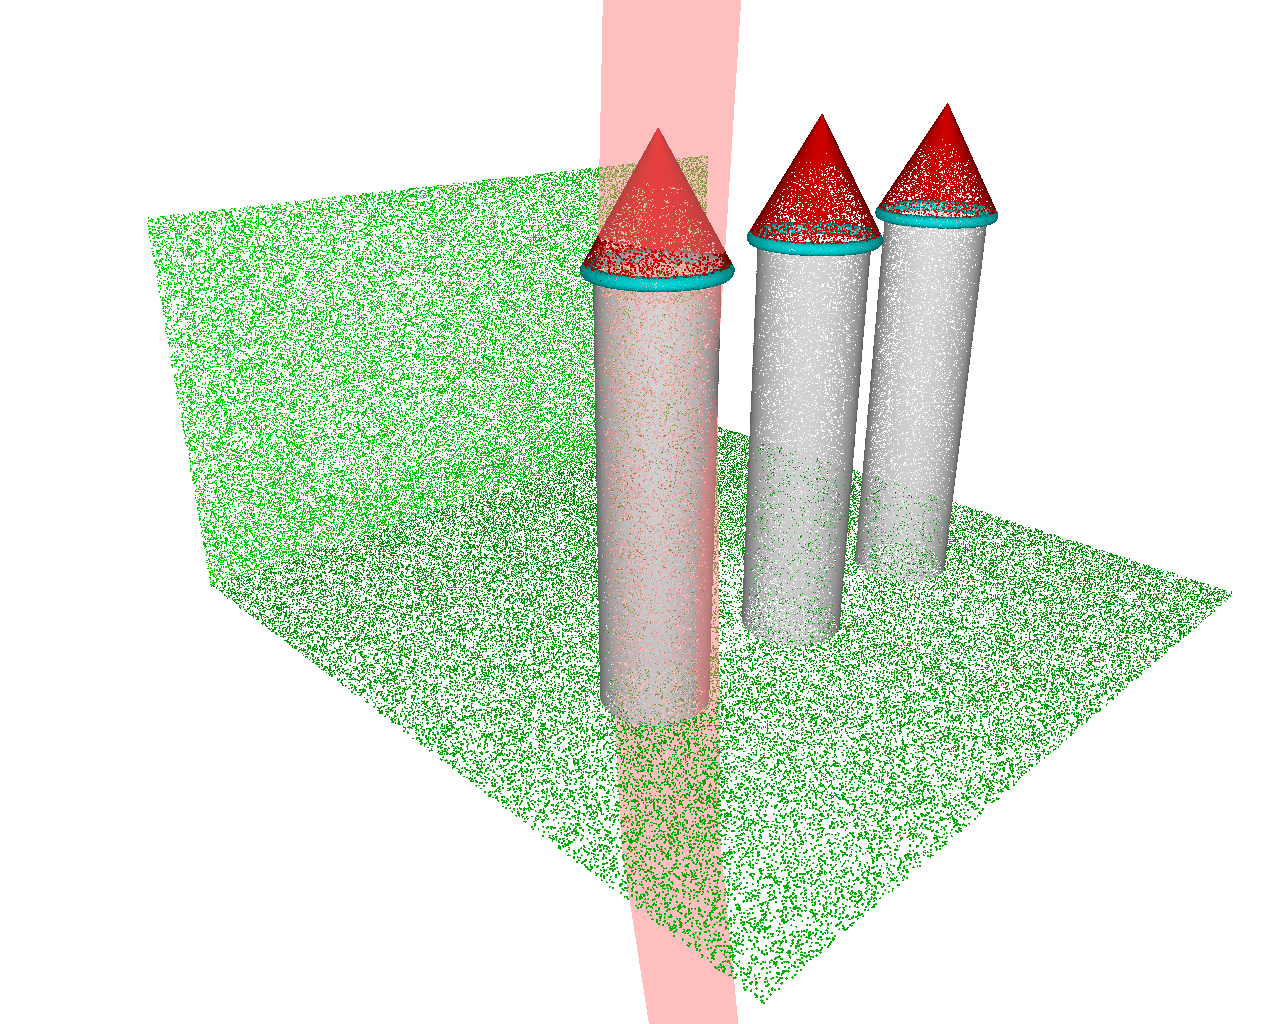
\includegraphics[width=0.49\textwidth]{Results/missfittedTorus1.png}%7
  }%\par\medskip
\subcaptionbox{ \label{fig:missfittedTorus2}}{%
  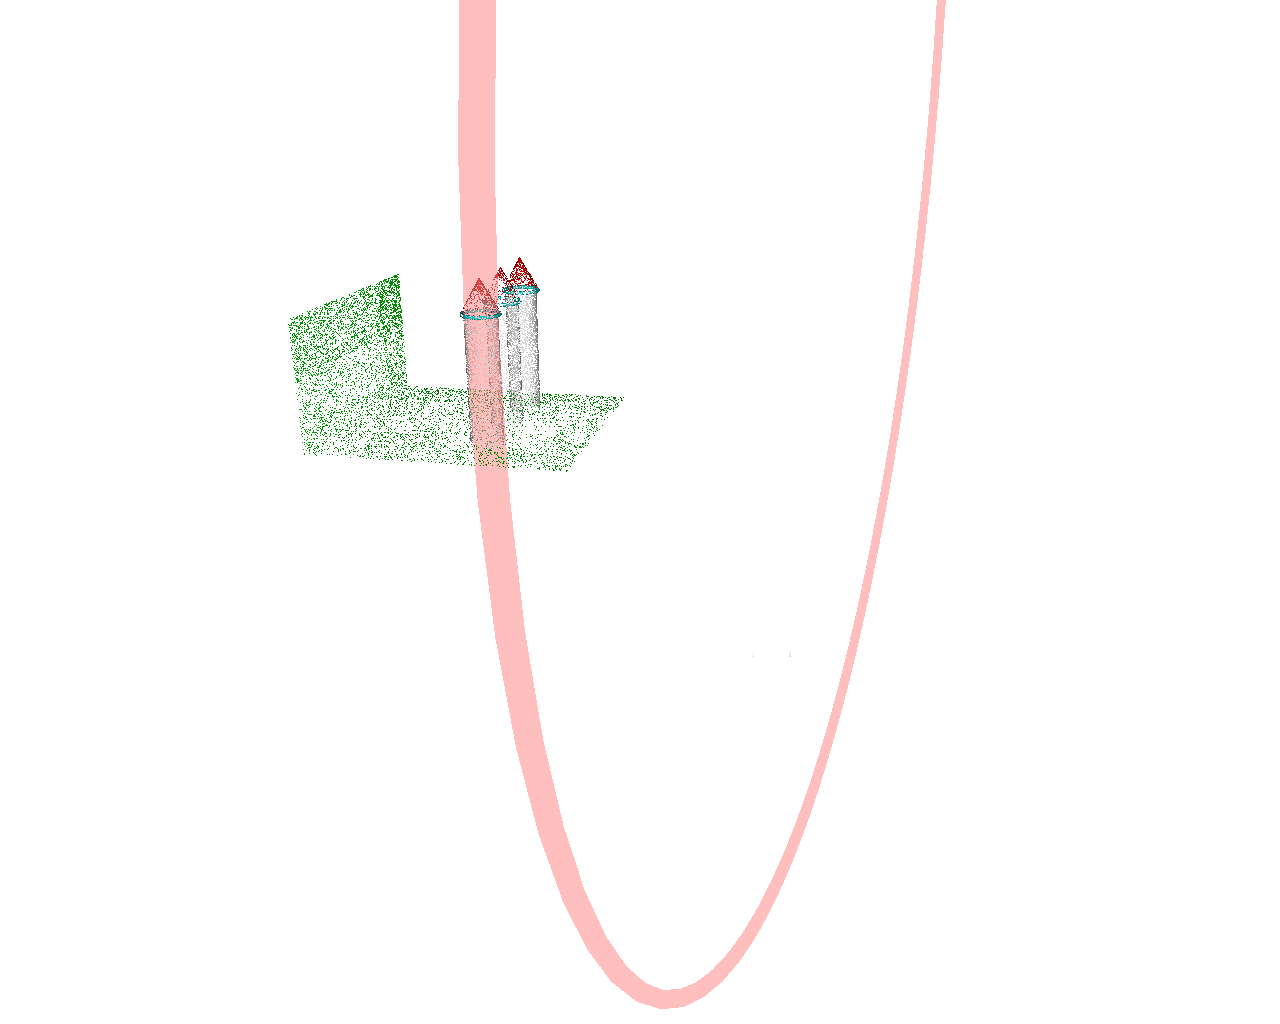
\includegraphics[width=0.49\textwidth]{Results/missfittedTorus2.png}%
  }      
\caption{This figure shows a cylinder from the synthetic point cloud whose points are classified as a torus instead of a cylinder. Even tough the points fit the torus, determined by the RANSAC options, the result is not plausible, since the user would expect a cylinder for this constellation of points. }
\label{fig:missfittedTorus}
\end{figure}


\subsection{Results}

This section presents results for the RANSAC shape detection performed on three data sets. The results in Figure \ref{fig:synthetic_point_cloud_results}, \ref{fig:JB_haus_results}, and \ref{fig:technologiezentrum_results} are obtained by segmenting the point clouds as a whole. Results for the interactive shape detection can be seen in Figure \ref{fig:technologiezentrum_interactive_shape_detection}. 

The synthetic test scene consists of two planes, three cylinders, three tori, and three cones.  Figure \ref{fig:synthetic_point_cloud_results} shows the synthetic point cloud, as well as the shapes that are detected within the point cloud. As the RANSAC approach randomly selects a subset of points, the results can be different for different runs. 

\begin{figure}[h]
\centering
\subcaptionbox{ \label{fig:synthetic_point_cloud}}{%
  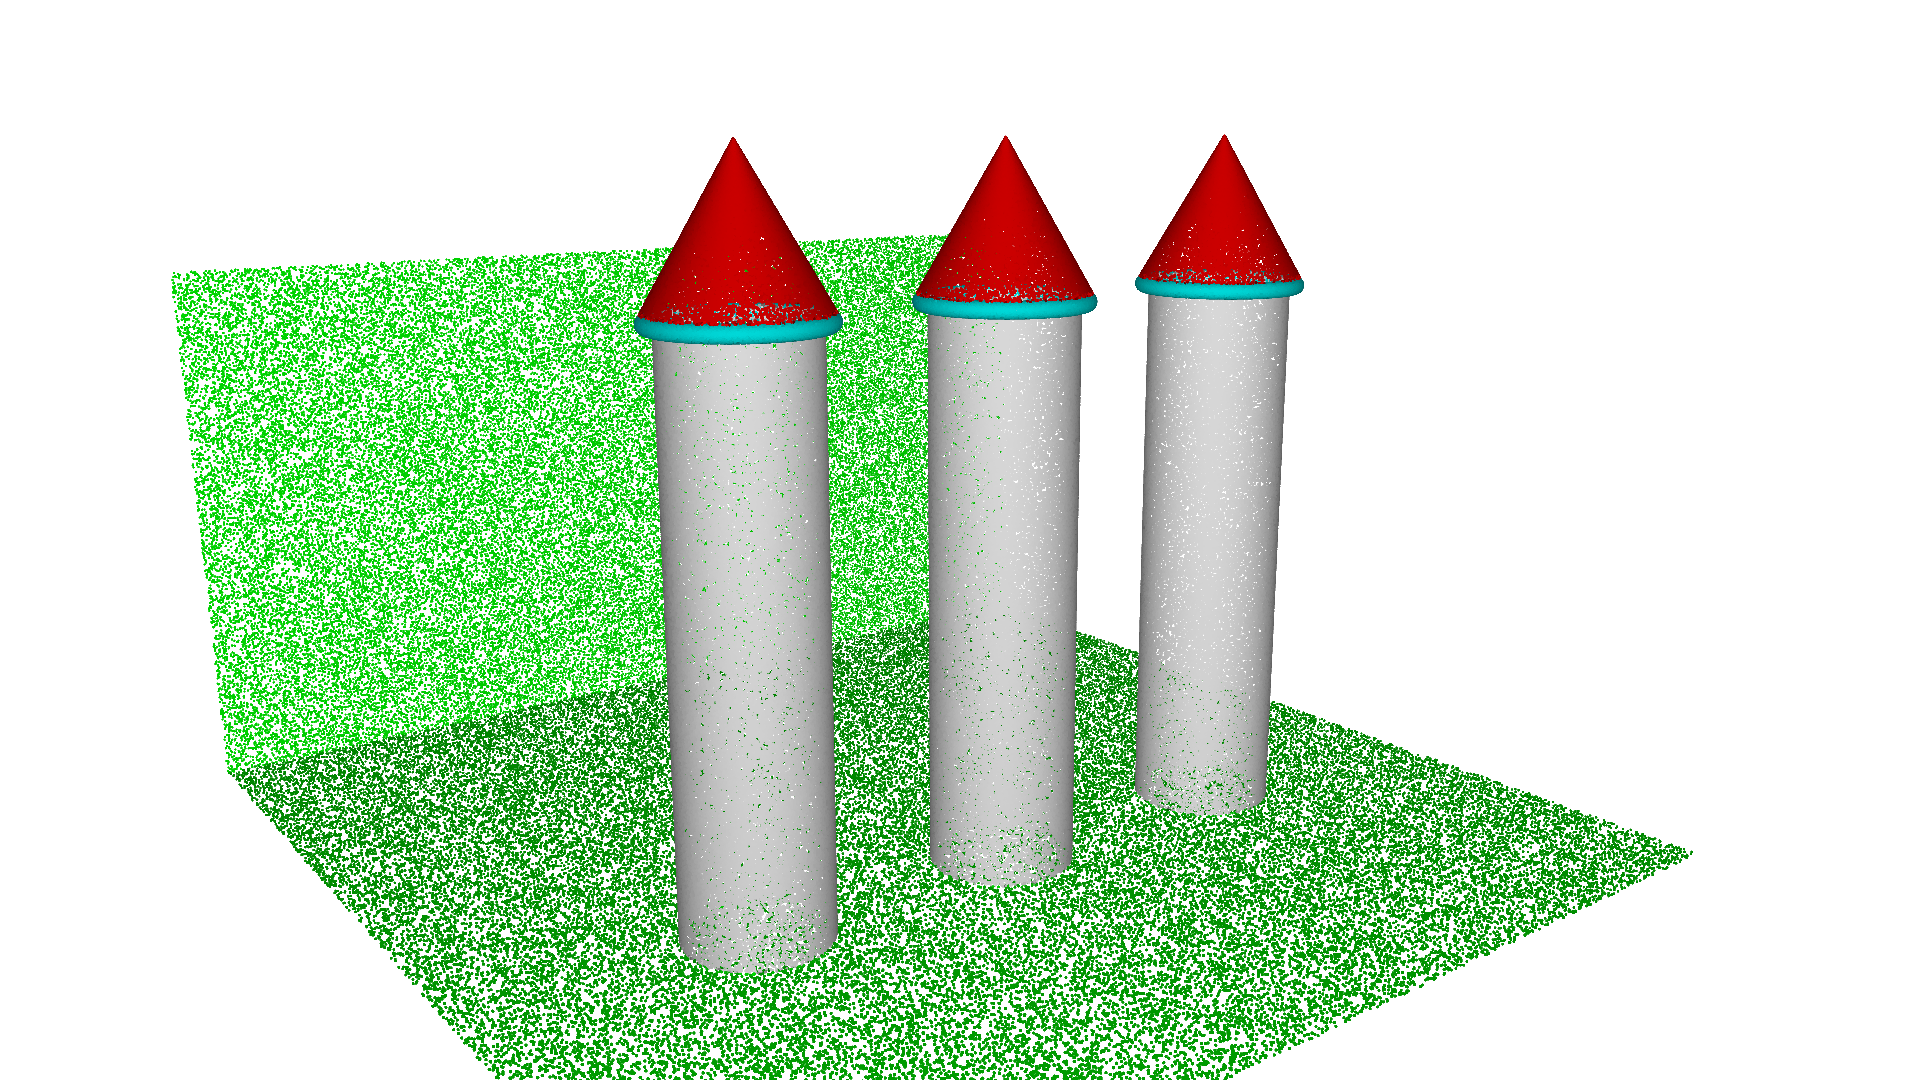
\includegraphics[width=0.7\textwidth]{Results/synthetic_point_cloud.png}%7
  }
\subcaptionbox{ \label{fig:synthetic_point_cloud_shapes}}{%
  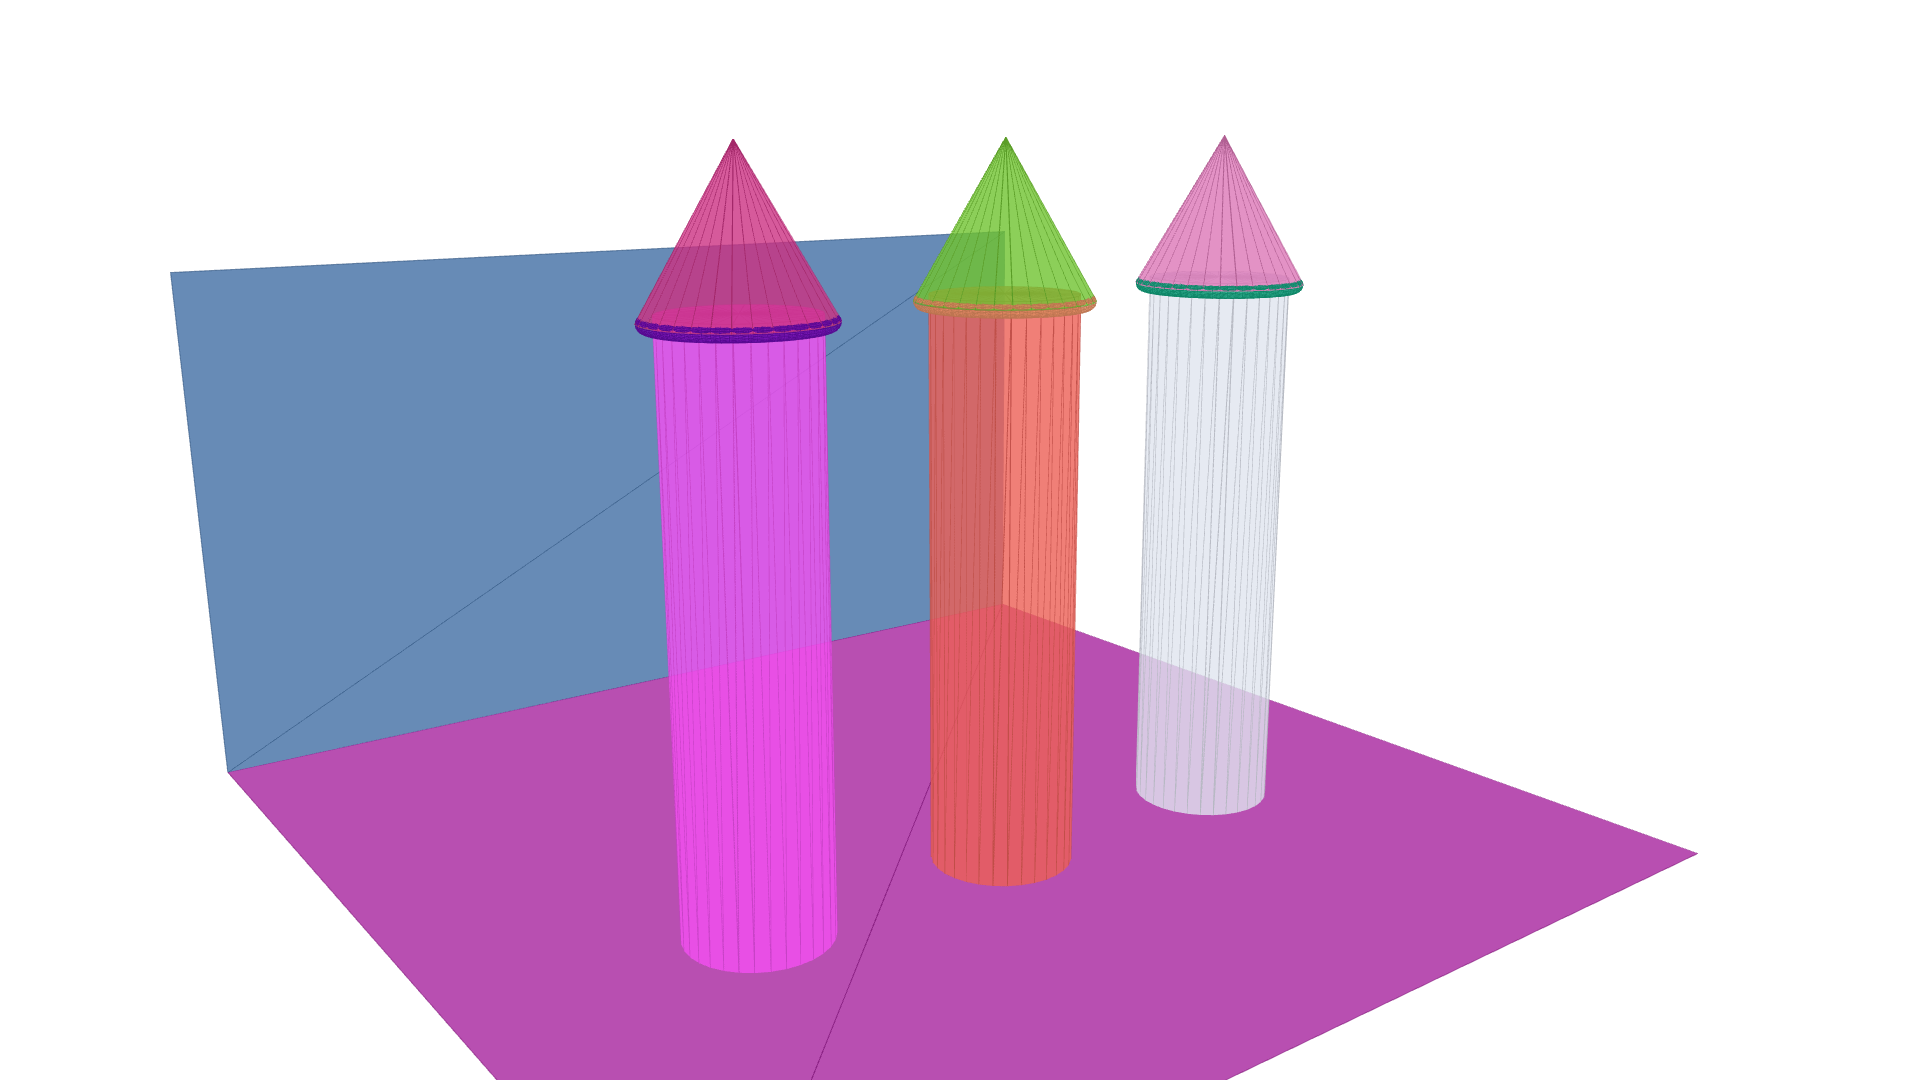
\includegraphics[width=0.7\textwidth]{Results/synthetic_point_cloud_shapes.png}%
  }
\caption{(a) shows the synthetic point cloud, consisting of two planes, three cylinders, three tori, and three cones. (b) shows the detected shapes rendered as triangle meshes. For each shape in the point cloud, the RANSAC shape detection has found a suitable primitive shape. }
\label{fig:synthetic_point_cloud_results}
\end{figure}

\begin{figure}
\centering
\subcaptionbox{ \label{fig:jb_haus}}{%
  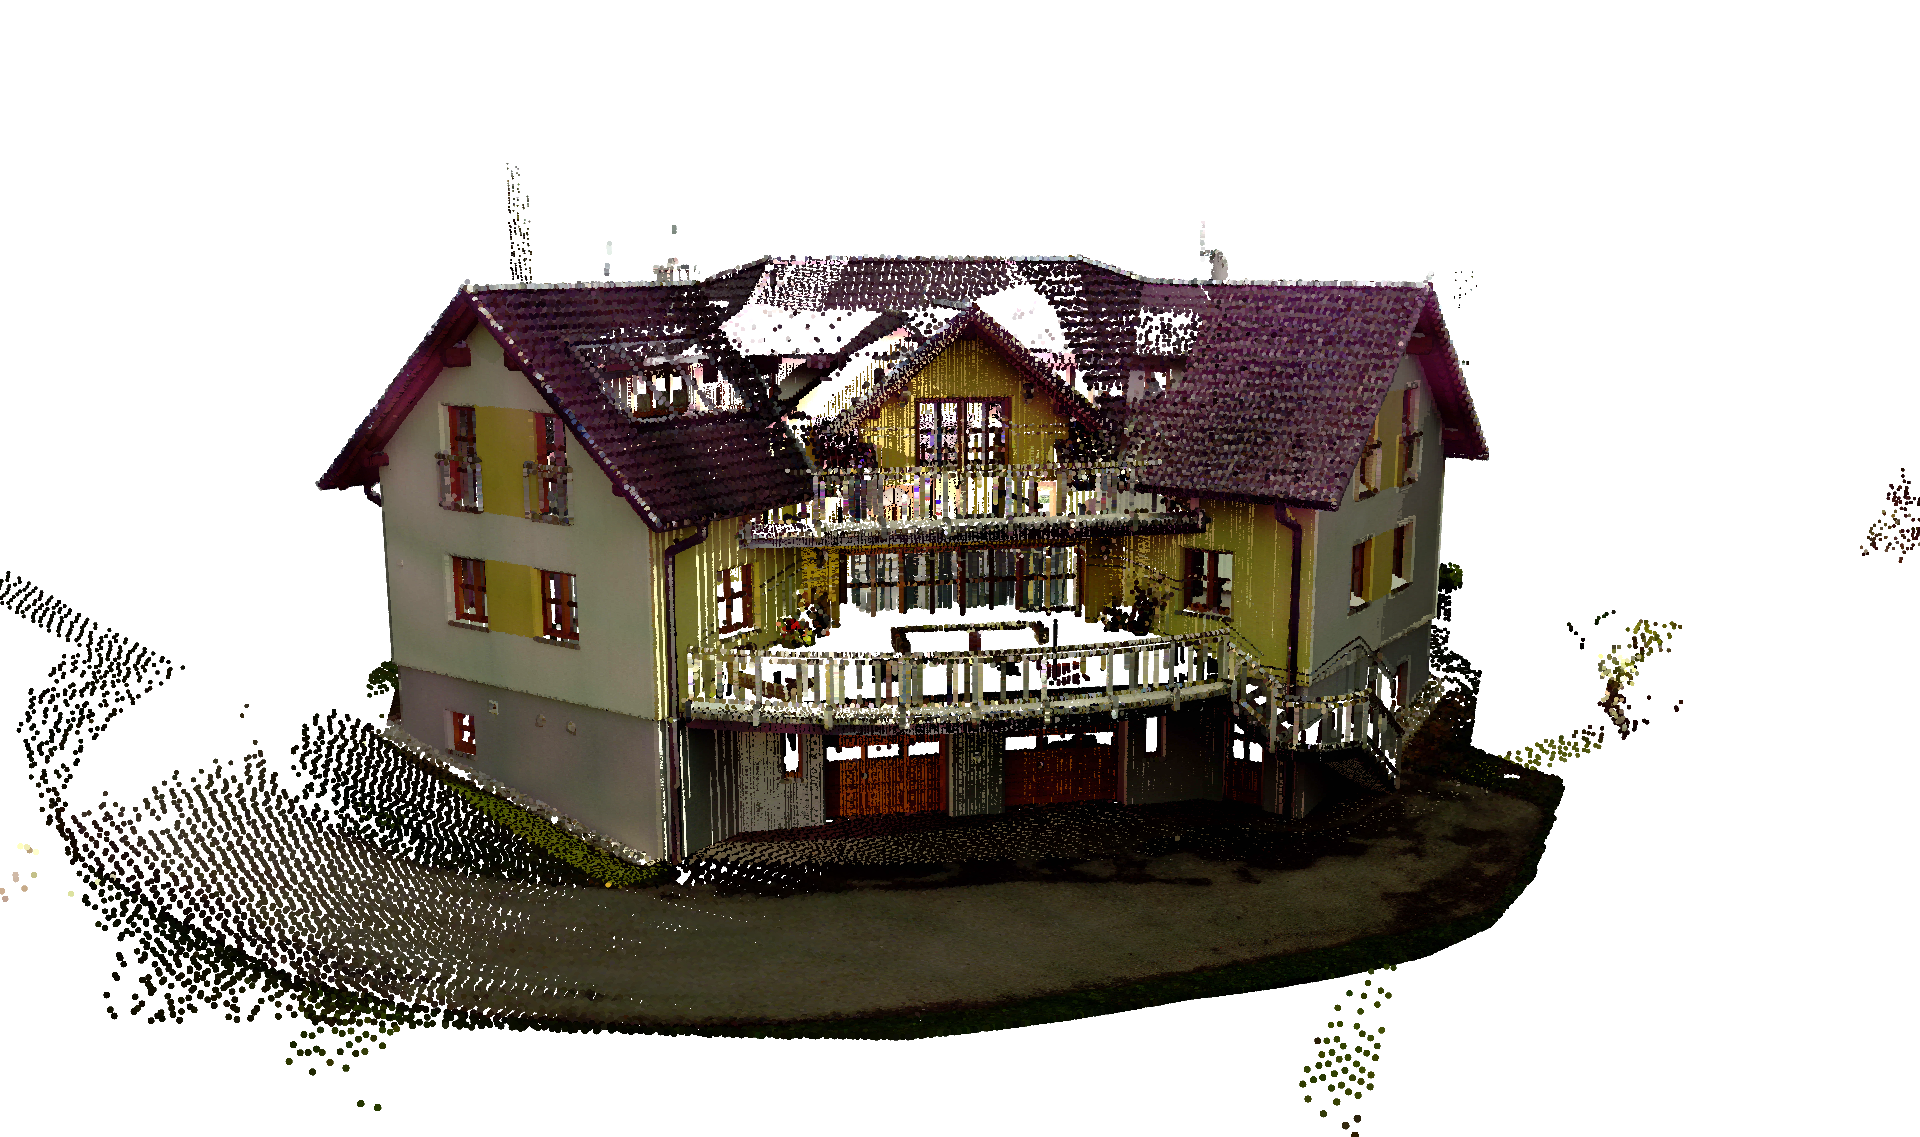
\includegraphics[width=\textwidth]{Results/jb_haus.png}%7
  }
\subcaptionbox{ \label{fig:jb_haus_shapes}}{%
  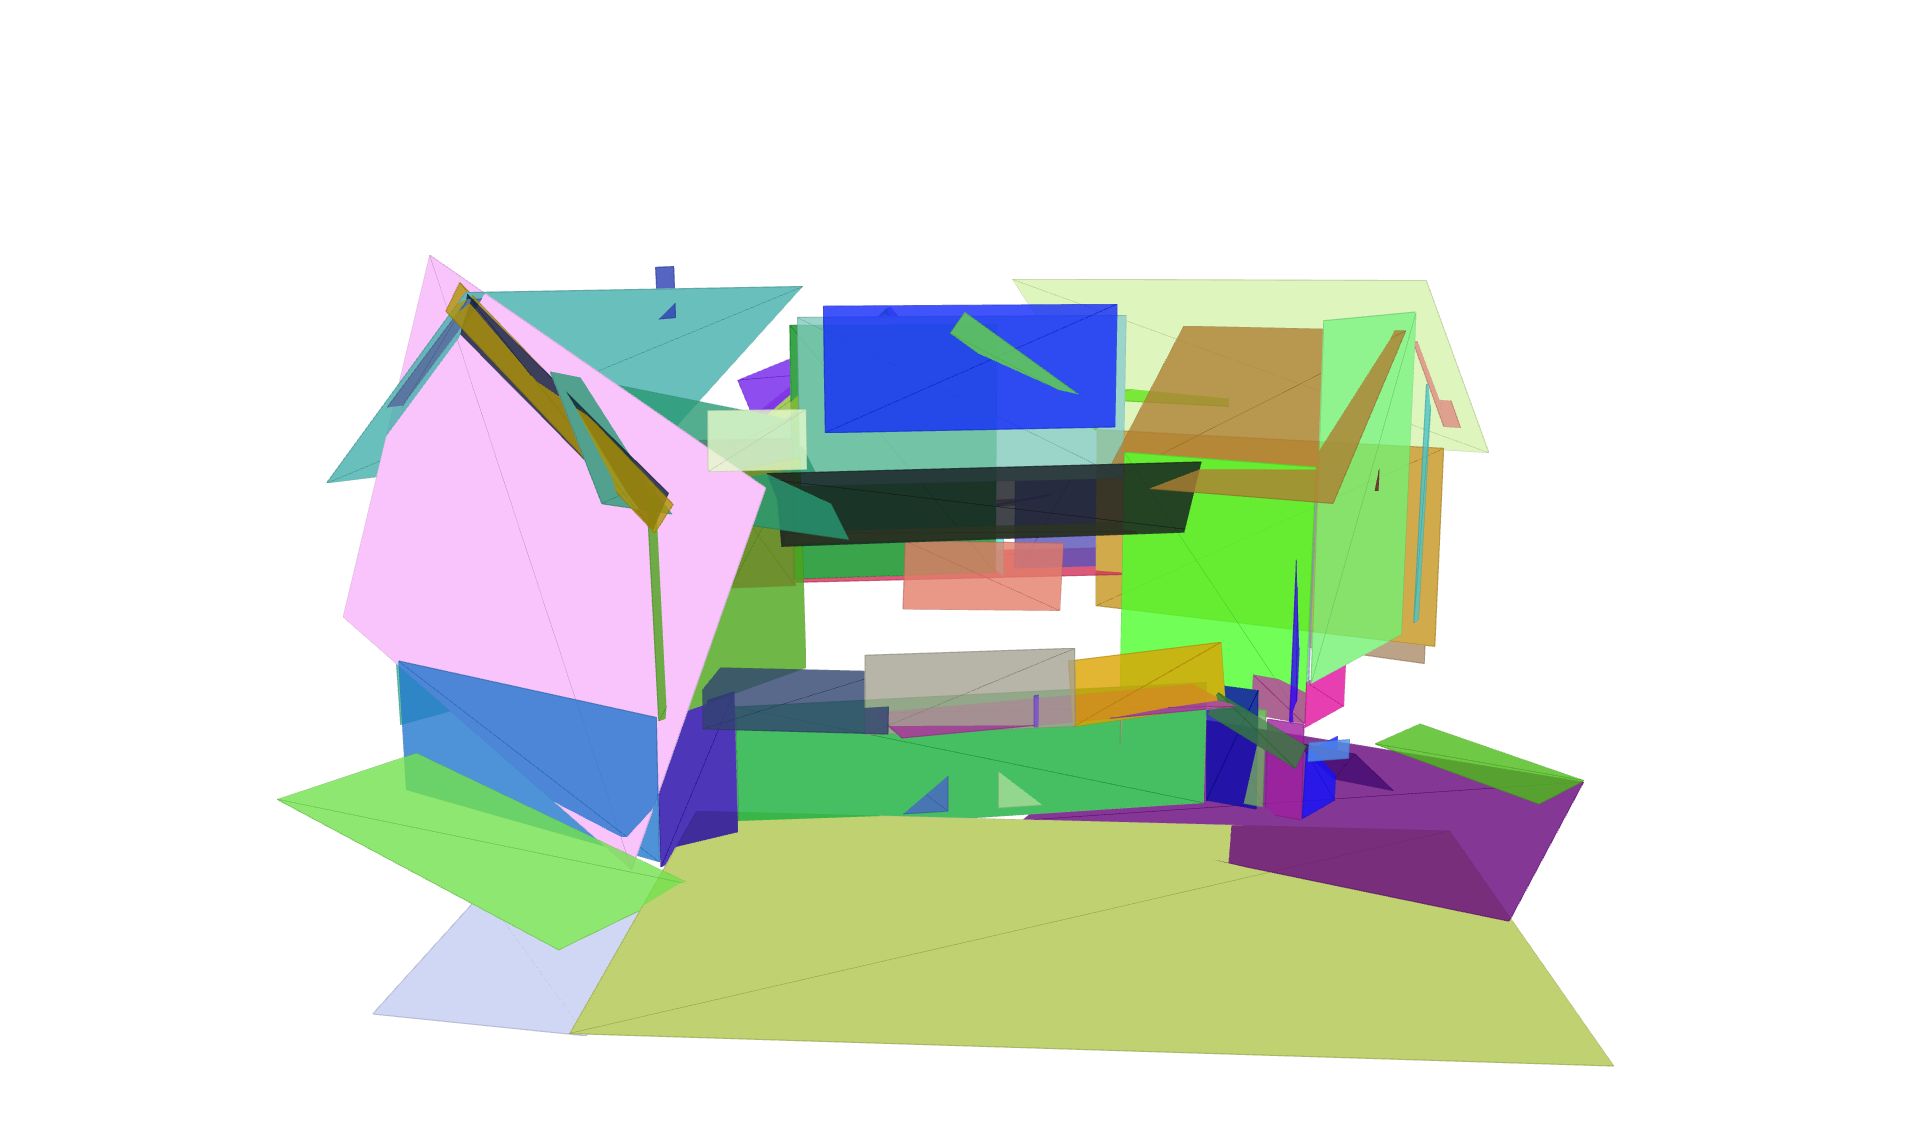
\includegraphics[width=\textwidth]{Results/jb_haus_shapes.png}%
  }
\caption{JB\_haus rendered as point cloud in (a), (b) shows all shapes detected in the point cloud. }
\label{fig:JB_haus_results}
\end{figure}

\begin{figure}
\centering
\subcaptionbox{ \label{fig:technologiezentrum}}{%
  \includegraphics[width=\textwidth]{Results/technologiezentrum.png}%7
  }
\subcaptionbox{ \label{fig:technologiezentrum_shapes}}{%
  \includegraphics[width=\textwidth]{Results/technologiezentrum_shapes.png}%
  }
\caption{Technologiezentrum rendered as point cloud in (a), (b) shows all shapes detected in the point cloud. }
\label{fig:technologiezentrum_results}
\end{figure}

\begin{figure}
\centering
\subcaptionbox{ \label{fig:technologiezentrum_interactive_shape_detection1}}{%
  \includegraphics[width=\textwidth]{Results/technologiezentrum_interactive_shape_detection1.png}%7
  }
\subcaptionbox{ \label{fig:technologiezentrum_interactive_shape_detection2}}{%
  \includegraphics[width=\textwidth]{Results/technologiezentrum_interactive_shape_detection2.png}%
  }
\caption{Based on the cursor's position a different shapes are selected. (a) and (b) show different shapes for different parts of the point cloud. Both shapes are a part of a wall. }
\label{fig:technologiezentrum_interactive_shape_detection}
\end{figure}


\section{Interaction Results}
\label{sec:interaction_results}

This section presents a set of figures that showcase the different interactions from Section \ref{sec:interactions}. The interactions are performed on the Technologiezentrum dataset since the JB\_Haus point cloud is used as an example throughout this thesis already. 

\begin{figure}[h]
\centering
\subcaptionbox{ \label{fig:technologiezentrum_lasso1}}{%
  \includegraphics[width=0.9\textwidth]{Results/technologiezentrum_lasso1.png}%7
  }
\subcaptionbox{ \label{fig:technologiezentrum_lasso2}}{%
  \includegraphics[width=0.9\textwidth]{Results/technologiezentrum_lasso2.png}%
  }
\caption{A lasso selection is performed on the selected support shape in (a). Only points are selected that lie on the support shape as shown in (b). Point in front and back of the support shape are not selected. }
\label{fig:technologiezentrum_lasso}
\end{figure}


\begin{figure}
\centering
\subcaptionbox{ \label{fig:technologiezentrum_brush1}}{%
  \includegraphics[width=\textwidth]{Results/technologiezentrum_brush1.png}%7
  }
\subcaptionbox{ \label{fig:technologiezentrum_brush2}}{%
  \includegraphics[width=\textwidth]{Results/technologiezentrum_brush2.png}%
  }
\caption{A volumetric brush selection is performed on the selected support shape in (a). Point are only selected if they belong to the support shape and intersect the brush. The result of the selection can be seen in (b).}
\label{fig:technologiezentrum_brush}
\end{figure}


\begin{figure}
\centering
\subcaptionbox{ \label{fig:technologiezentrum_lod_increment1}}{%
  \includegraphics[width=\textwidth]{Results/technologiezentrum_lod_increment1.png}%7
  }
\subcaptionbox{ \label{fig:technologiezentrum_lod_increment2}}{%
  \includegraphics[width=\textwidth]{Results/technologiezentrum_lod_increment2.png}%
  }
\caption{The \textit{level-of-detail} is incremented along the support shape. (a) shows the original rendering model of the point cloud, (b) shows the point cloud with additional points. }
\label{fig:technologiezentrum_lod_increment}
\end{figure}





\chapter{Conclusion and Future Work}
\label{chap:conclusion}


This chapter completes this thesis by presenting a conclusion on the work and proposing future work.

\subsection*{Out-of-core Representation of Point Clouds}

Modern point clouds often consist of several billion points and consume several gigabytes of memory. They are simply too large to fit into system memory as a whole. This thesis describes a functional octree structure that can handle the out-of-core functionality of the point cloud. Data is stored in chunks in a file and is loaded into system memory when needed. Additionally, the point cloud's octree nodes contain a subset of points from its children, thus creating a multi-scale representation of the point cloud that is used for rendering and interactions. 


\subsection*{User-Guided Shape Detection}

This thesis shows an alternative use of the shape detection algorithm by Schnabel et al. \cite{schnabel-2007-efficient} which lets the user control the regions that are segmented. By pointing to a region with the mouse, the system selects the most suitable octree node to be segmented. The octree's split decision ensures a consistent number of points per shape, such that the shape detection delivers results in interactive time. The shape detection is performed on the highest visible level of detail. Hence, this approach creates a multi-scale representation of the shapes by performing shape detection on nodes with different level of detail. To account for different point distributions in octree nodes, a dynamic $\epsilon$ threshold, based on the node's point density, is proposed for the shape detection. 


\subsection*{Improvement of Interaction Techniques}

Several improvements to well-known two-dimensional interaction techniques are discussed in this thesis. We propose a way of pre-filtering points for interactions such that only points are considered that are approximated by a support shape, picked by the user. Classic point picking is improved such that only points are picked that belong to the support shape. Only using points that belong to a shape is especially useful when trying to pick points that are otherwise occluded or lie on the edge of a structure. Multiple ways exist to select regions in a point cloud. We utilize a support shape to improve the lasso selection. Classic lasso selection selects all points, whose projection lies inside the lasso on the near plane. The user selects ´through´ the point cloud, whereas when using a support shape, the user only selects points that lie on this support shape. The volumetric brush allows the user to select points that are in the foreground. Instead of consulting the depth buffer to retrieve the brush's position, the position of the cursor on the support shape is used. Thus, the brush does not follow the structures that are in the foreground but the curvature of the support shape and points can be selected that are occluded otherwise. 


\subsection*{Novel Interaction to Magnify Local Details}

The final task of this thesis was to design a novel interaction technique called \textit{shape-assisted local level-of-detail increment}. The level-of-detail rendering of the point cloud displays only a subset of points that can be rendered by the graphics card in real time. Thus, details may get culled and are not rendered. The interaction technique collects points from nodes that are not rendered due to their level-of-detail. These additional points follow the curvature of the support shape. Along the support shape, extra points are rendered that would otherwise be culled, therefore, allowing the user to get a more detailed look at structures. 


\section{Future Work}

As the focus of this thesis was the design of the user-guided shape detection and the assisted interactions, future work will focus on performance and robustness improvements on various fronts. The usage of a selection data structure, such as a selection octree \cite{scheiblauer2011out}, can improve the performance when selecting or editing the point cloud. Also, different ways can be explored to improve computation speed by taking advantage of the parallel architecture of the graphics card. 

\par

As the selection processing is performed asynchronously, feedback is not displayed immediately, but with a delay. To overcome this delay between interaction and receiving the result, a visual selection can be performed on the GPU \cite{rainer2016visual} to bridge this gap. This technique utilizes volumetric shadows to create a visual selection using the GPU's stencil buffer. 

\par

Shape detection is performed using an external library by Schnabel et al. \cite{schnabel-2007-software}. Multiple problems occur, such as non-termination or non-plausible shape matching. More work must be carried out to limit or eliminate these problems. The robustness of the shape detection, especially when detecting non-planar primitive shapes, suffers due to weak constraints. Alternatively, the shape detection can be implemented in such a way, that particular types of shapes are prioritized to reduce the amount of non-plausible shapes. 

\par

In the current application, edges between nodes with different level of detail are visible. Regions with sparse points contain visible gaps. Adaptive point size \cite{scheiblauer-thesis} can be used to reduce the visual artifacts that come with this type of level-of-detail rendering. The individual point size for each octree node is controlled by the number of points and weighted level of detail. 


%instead of taking samples, average samples bei octree aufbau%

\backmatter

% Use an optional list of figures.
\listoffigures % Starred version, i.e., \listoffigures*, removes the toc entry.

% Use an optional list of tables.
\cleardoublepage % Start list of tables on the next empty right hand page.
\listoftables % Starred version, i.e., \listoftables*, removes the toc entry.

% Use an optional list of alogrithms.
\listofalgorithms
\addcontentsline{toc}{chapter}{List of Algorithms}

% Add an index.
\printindex

% Add a glossary.
\printglossaries

% Add a bibliography.
\bibliographystyle{alpha}
\bibliography{intro}

\end{document}